\documentclass{beamer}
\title{What Every Programmer Should Know About Memory}
\author{Lars Quentin}
\date{15.11.2023}
\usetheme[numbering=none]{metropolis}
\usepackage{xcolor}
\begin{document}

% - Ein PC hat auf jeden Fall ein Prozessor, auch CPU genannt.
%   - CPU == Central Processing Unit == Zentrale Verarbeitungseinheit
%   - Der CPU hat
%     - Ein Rechenwerk, was die eigentlichen Instruktionen ausfuehrt
%     - Ein Steuerwerk, die sich um den Ablauf der Instruktionen kuemmert
%     - Register, welche meist 8 byte kleine, sehr schnelle Speicher fuer das Rechenwerk sind.
%   - Und noch vieles mehr, wie ein Speichermanager (Memory Management Unit) oder caches oder ne clock.
\begin{frame}[t]
\frametitle{Wie ist ein PC aufgebaut?}
\pause
\centering
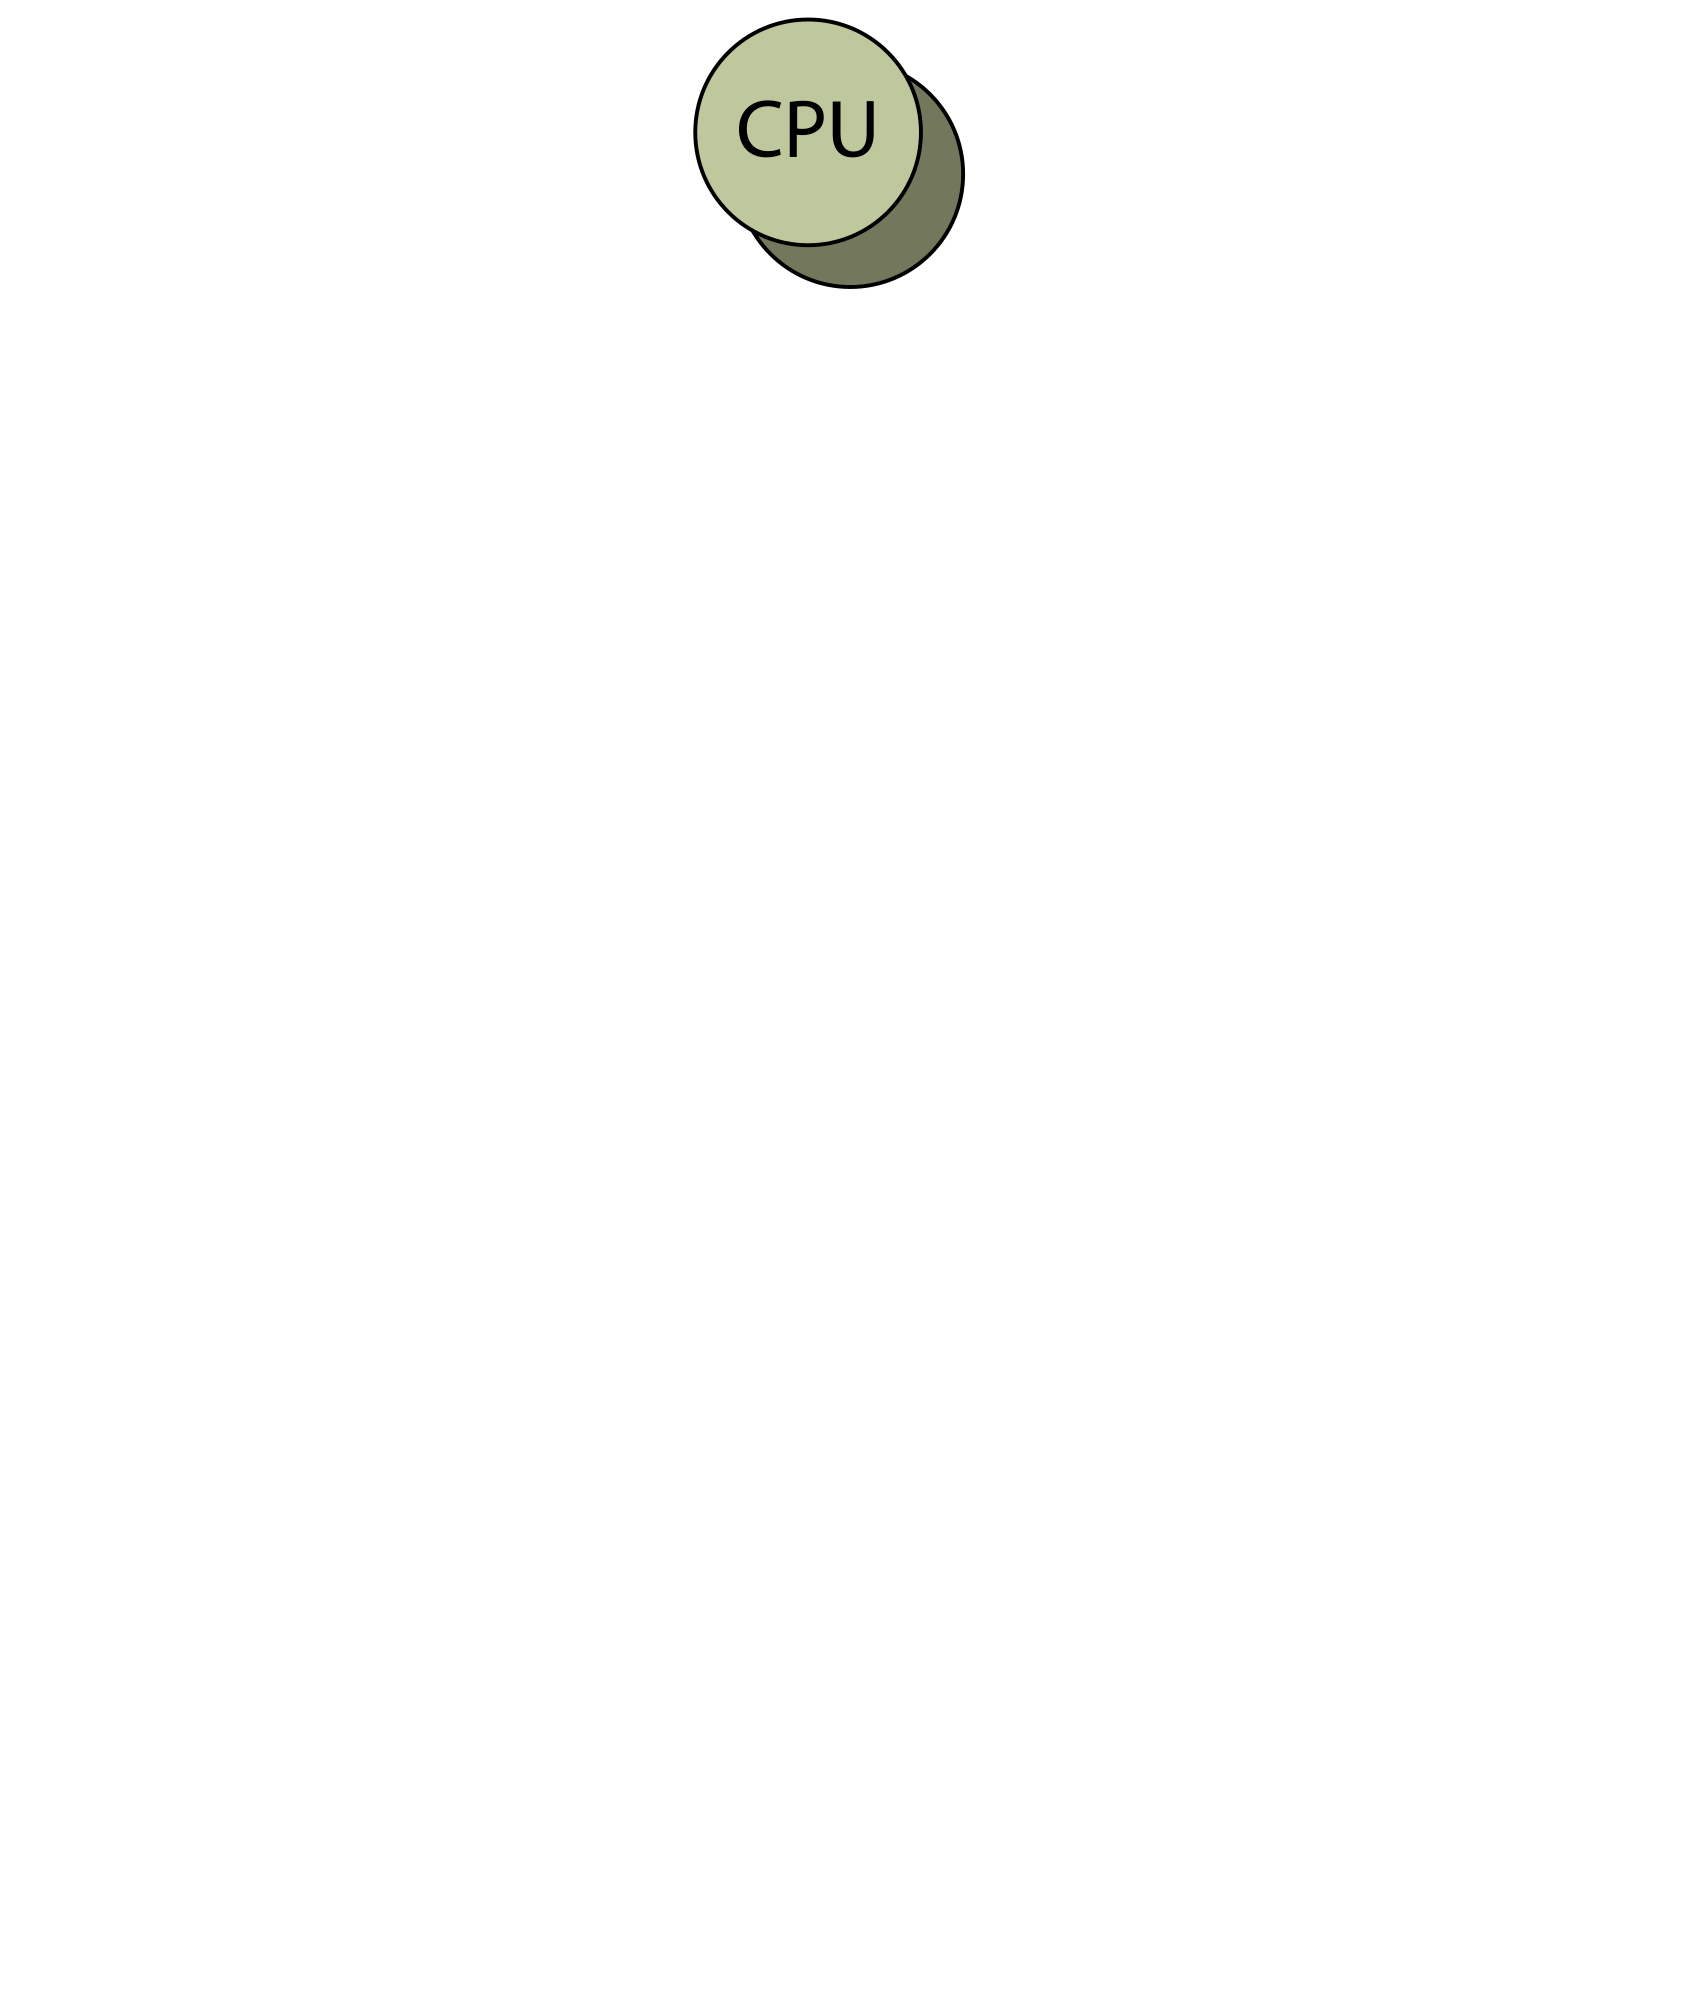
\includegraphics[width=7cm]{architecture1.png}
\end{frame}

% - Der CPU ist durch Front Side Bus (FSB) mit dem
\begin{frame}[t]
\frametitle{Wie ist ein PC aufgebaut?}
\centering
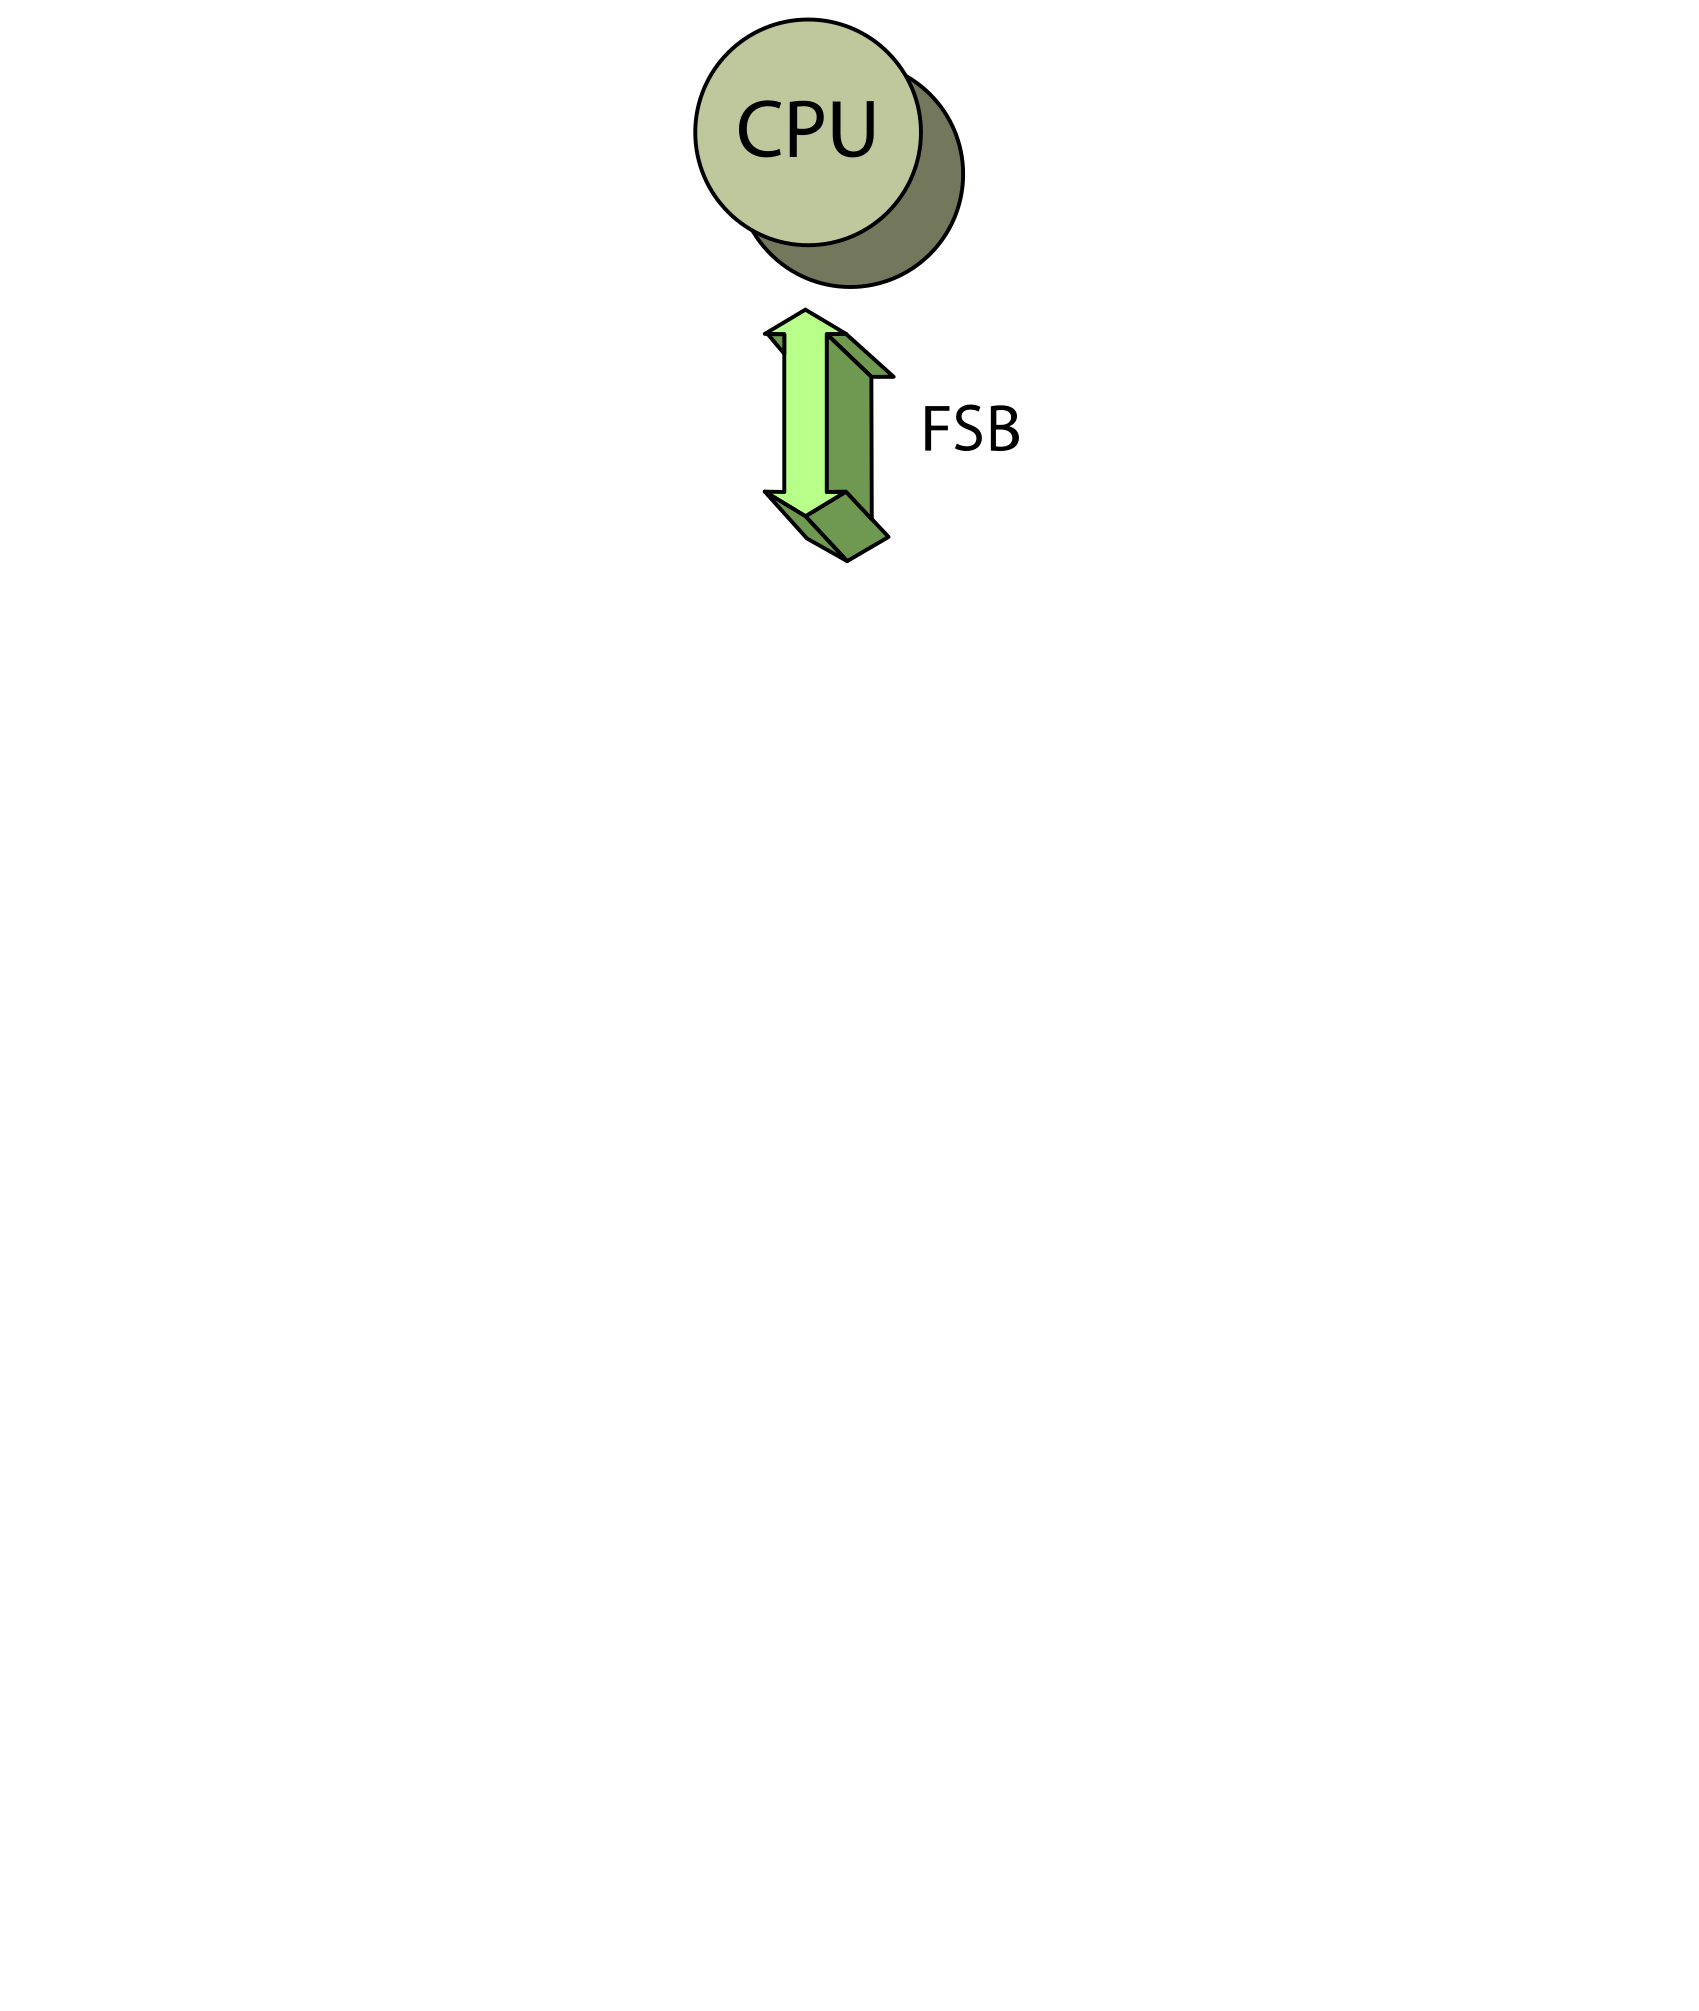
\includegraphics[width=7cm]{architecture2.png}
\end{frame}

% - Northbridge Chip verbunden.
%   - Auf modernen Rechnern befindet sich der FSB sowie North Bridge mit auf der CPU-Platine.
%   - Bei Intel ist es wirklich auf im Prozessor drin, AMD rockt mit Zen 2 eine Mikroprozessorarchitektur wo
%     die North bridge noch getrennt ist.
%   - Die Northbridge kuemmert sich um moeglichst schnellen Datentransfer mit anderen Komponenten,
%     insbesondere dem
\begin{frame}[t]
\frametitle{Wie ist ein PC aufgebaut?}
\centering
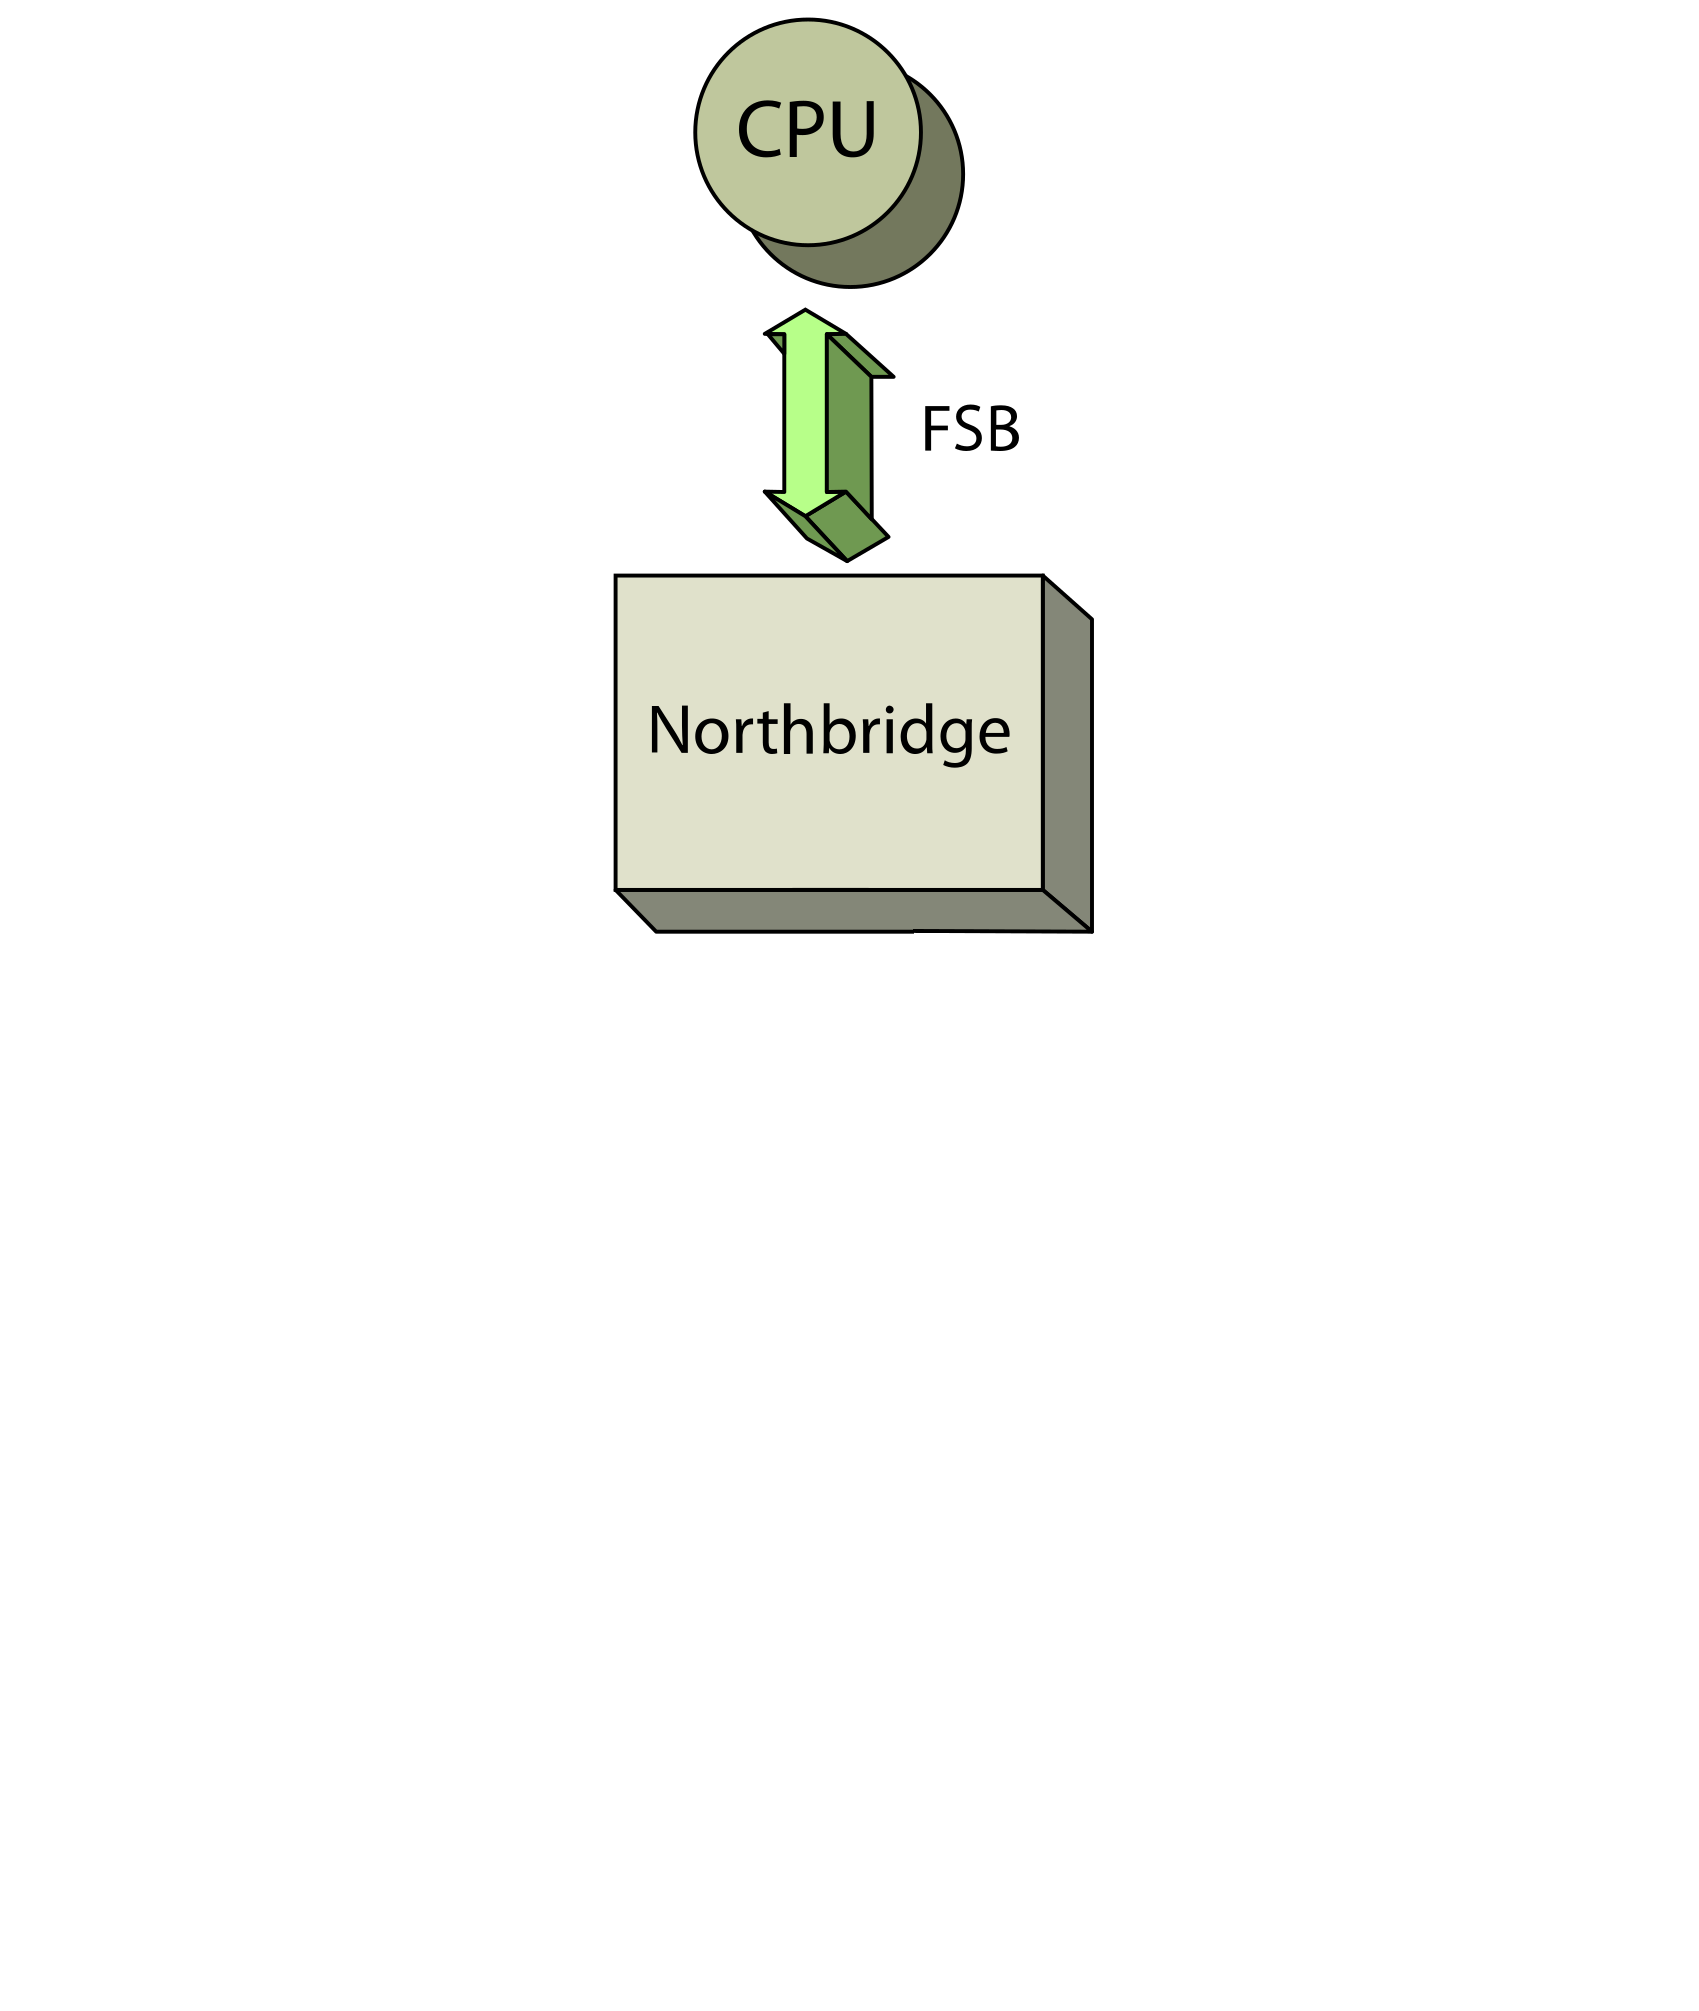
\includegraphics[width=7cm]{architecture3.png}
\end{frame}

% - RAM (Random Access Memory), was der Arbeitsspeicher ist.
%   - Der ist in der Groesse von ein paar GB, bei mir 24GB.
%   - Wie der Name Arbeits Speicher bereits verraet, ist das der Speicher mit dem der PC aktiv arbeitet, weil
%     er entgegen einer Festplatte schnell genug ist.
%   - Die Festplatte waere dafuer zu langsam, wie wir spaeter noch sehen werden.
% - Zudem sind dort alle
\begin{frame}[t]
\frametitle{Wie ist ein PC aufgebaut?}
\centering
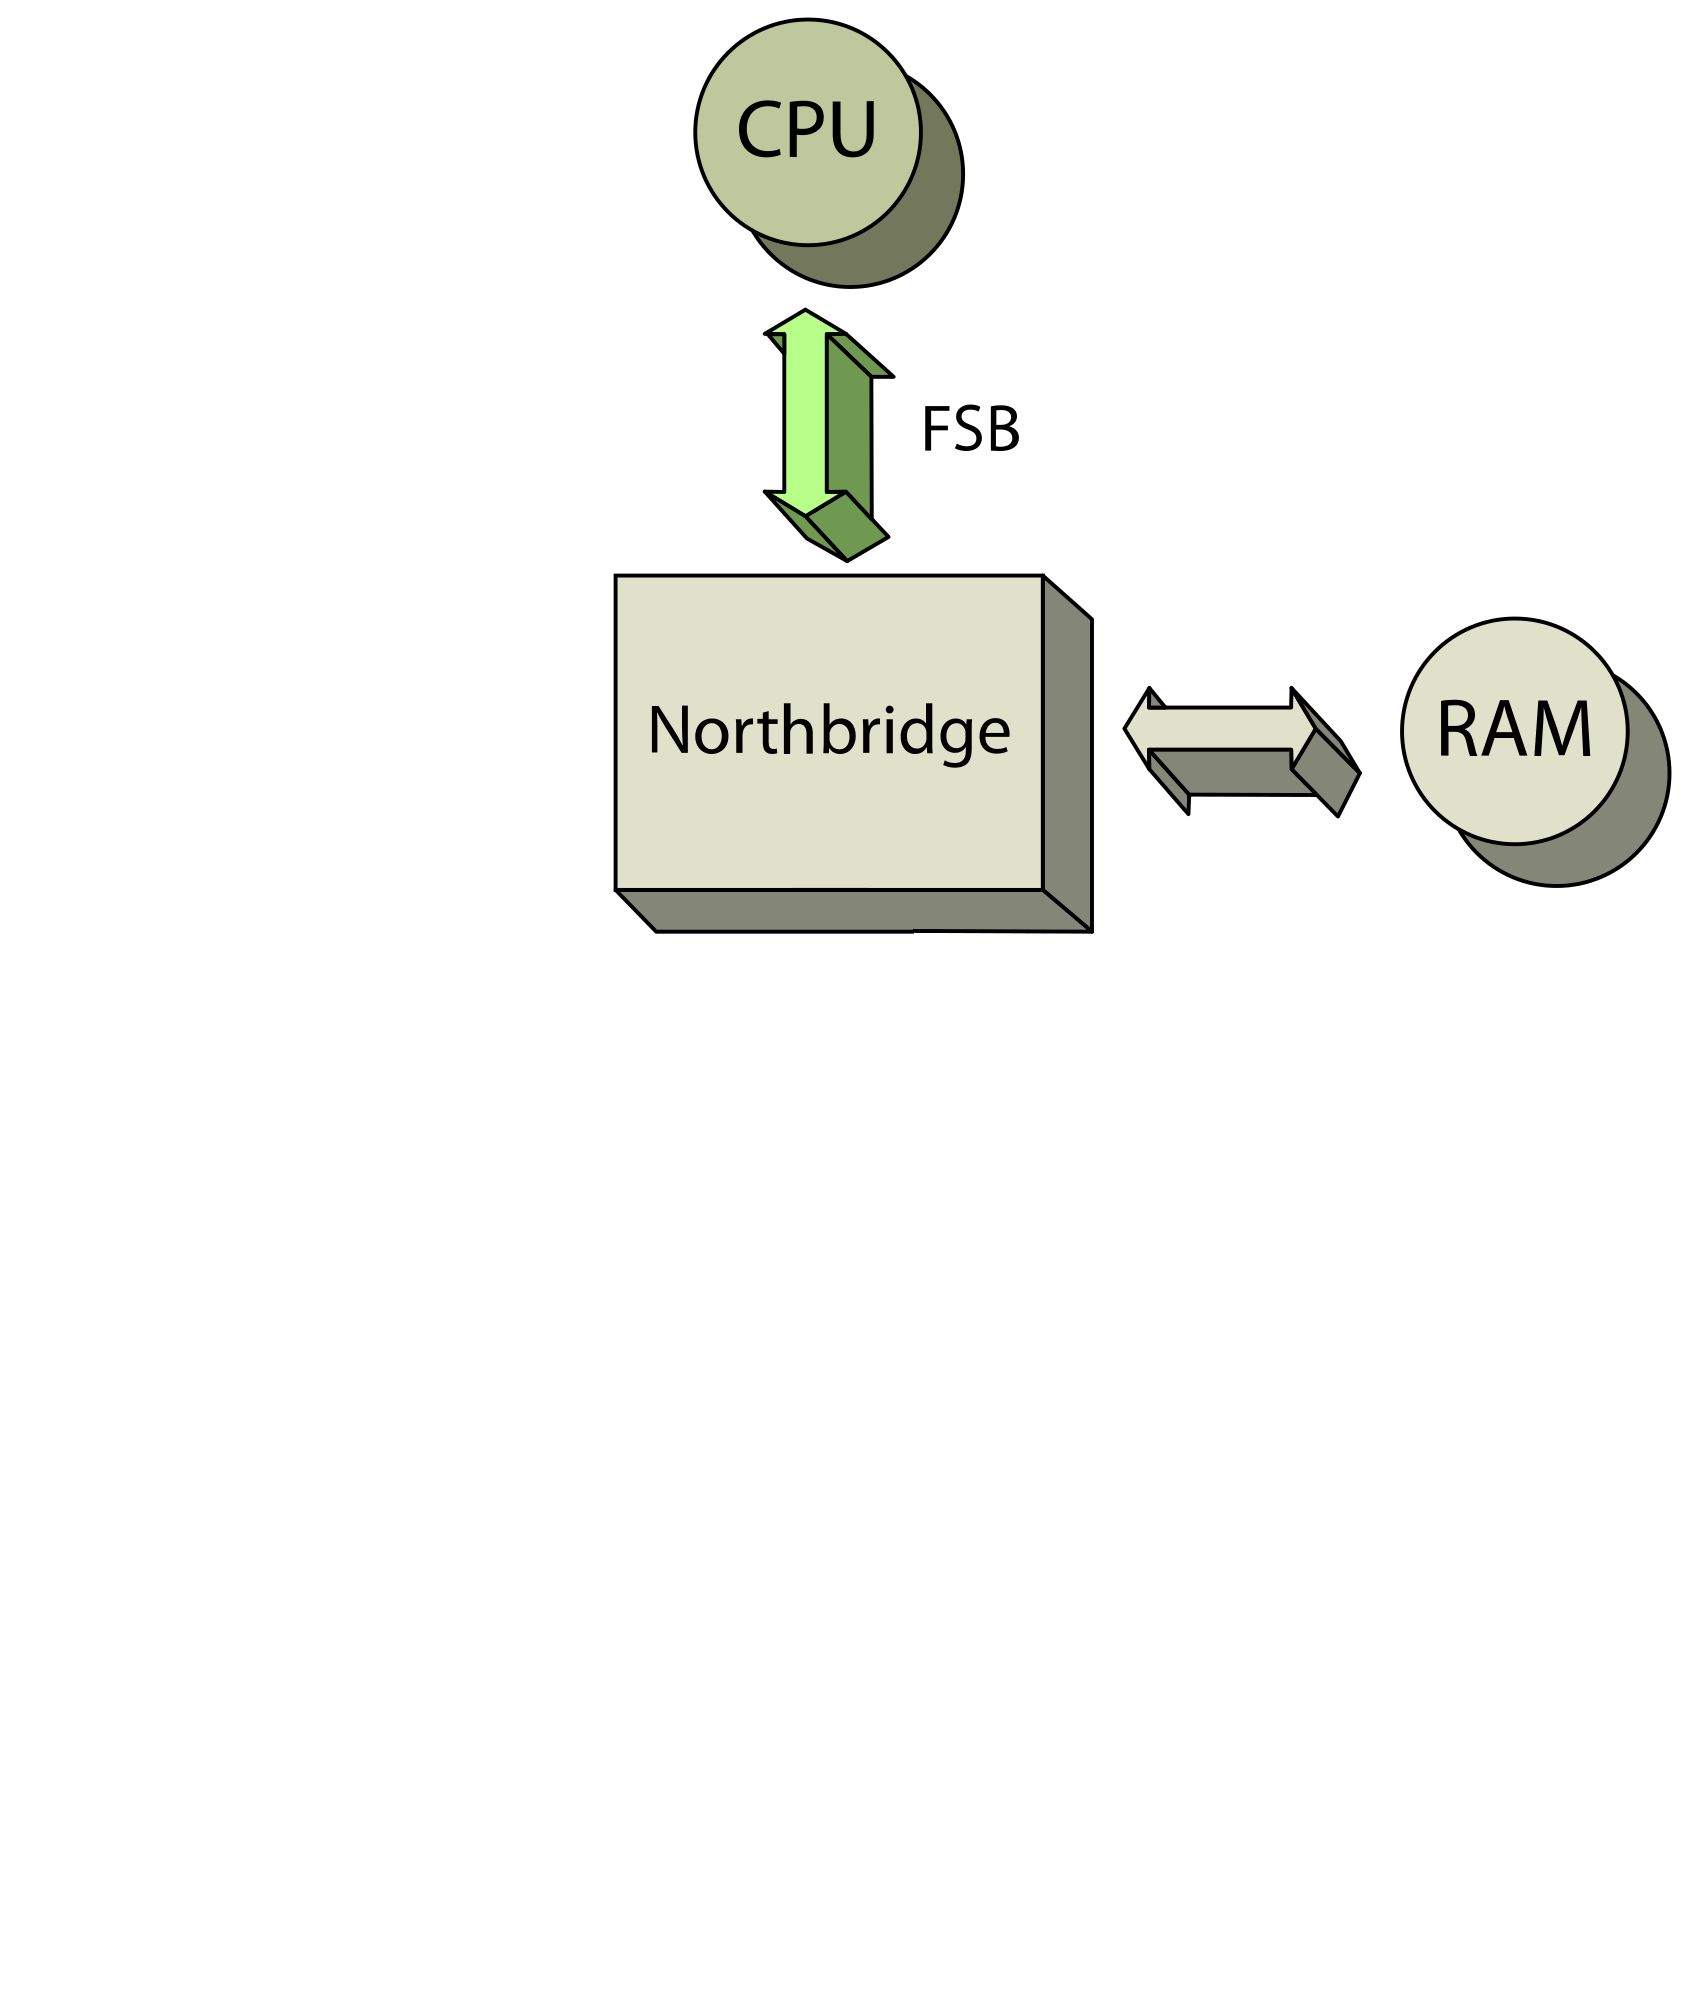
\includegraphics[width=7cm]{architecture4.png}
\end{frame}

% - PCIe-Geraete angeschlossen. (PCI ist der Anschluss) (PCI == Peripheral Component Interconnect)
%   - Effektiv sind das meistens Grafikkarten oder High Performance Netzwerkkarten.
% - Also bei der Northbridge sind die zeitlich schnellen Sachen angebunden. Die Northbridge ist dann mit der
\begin{frame}[t]
\frametitle{Wie ist ein PC aufgebaut?}
\centering
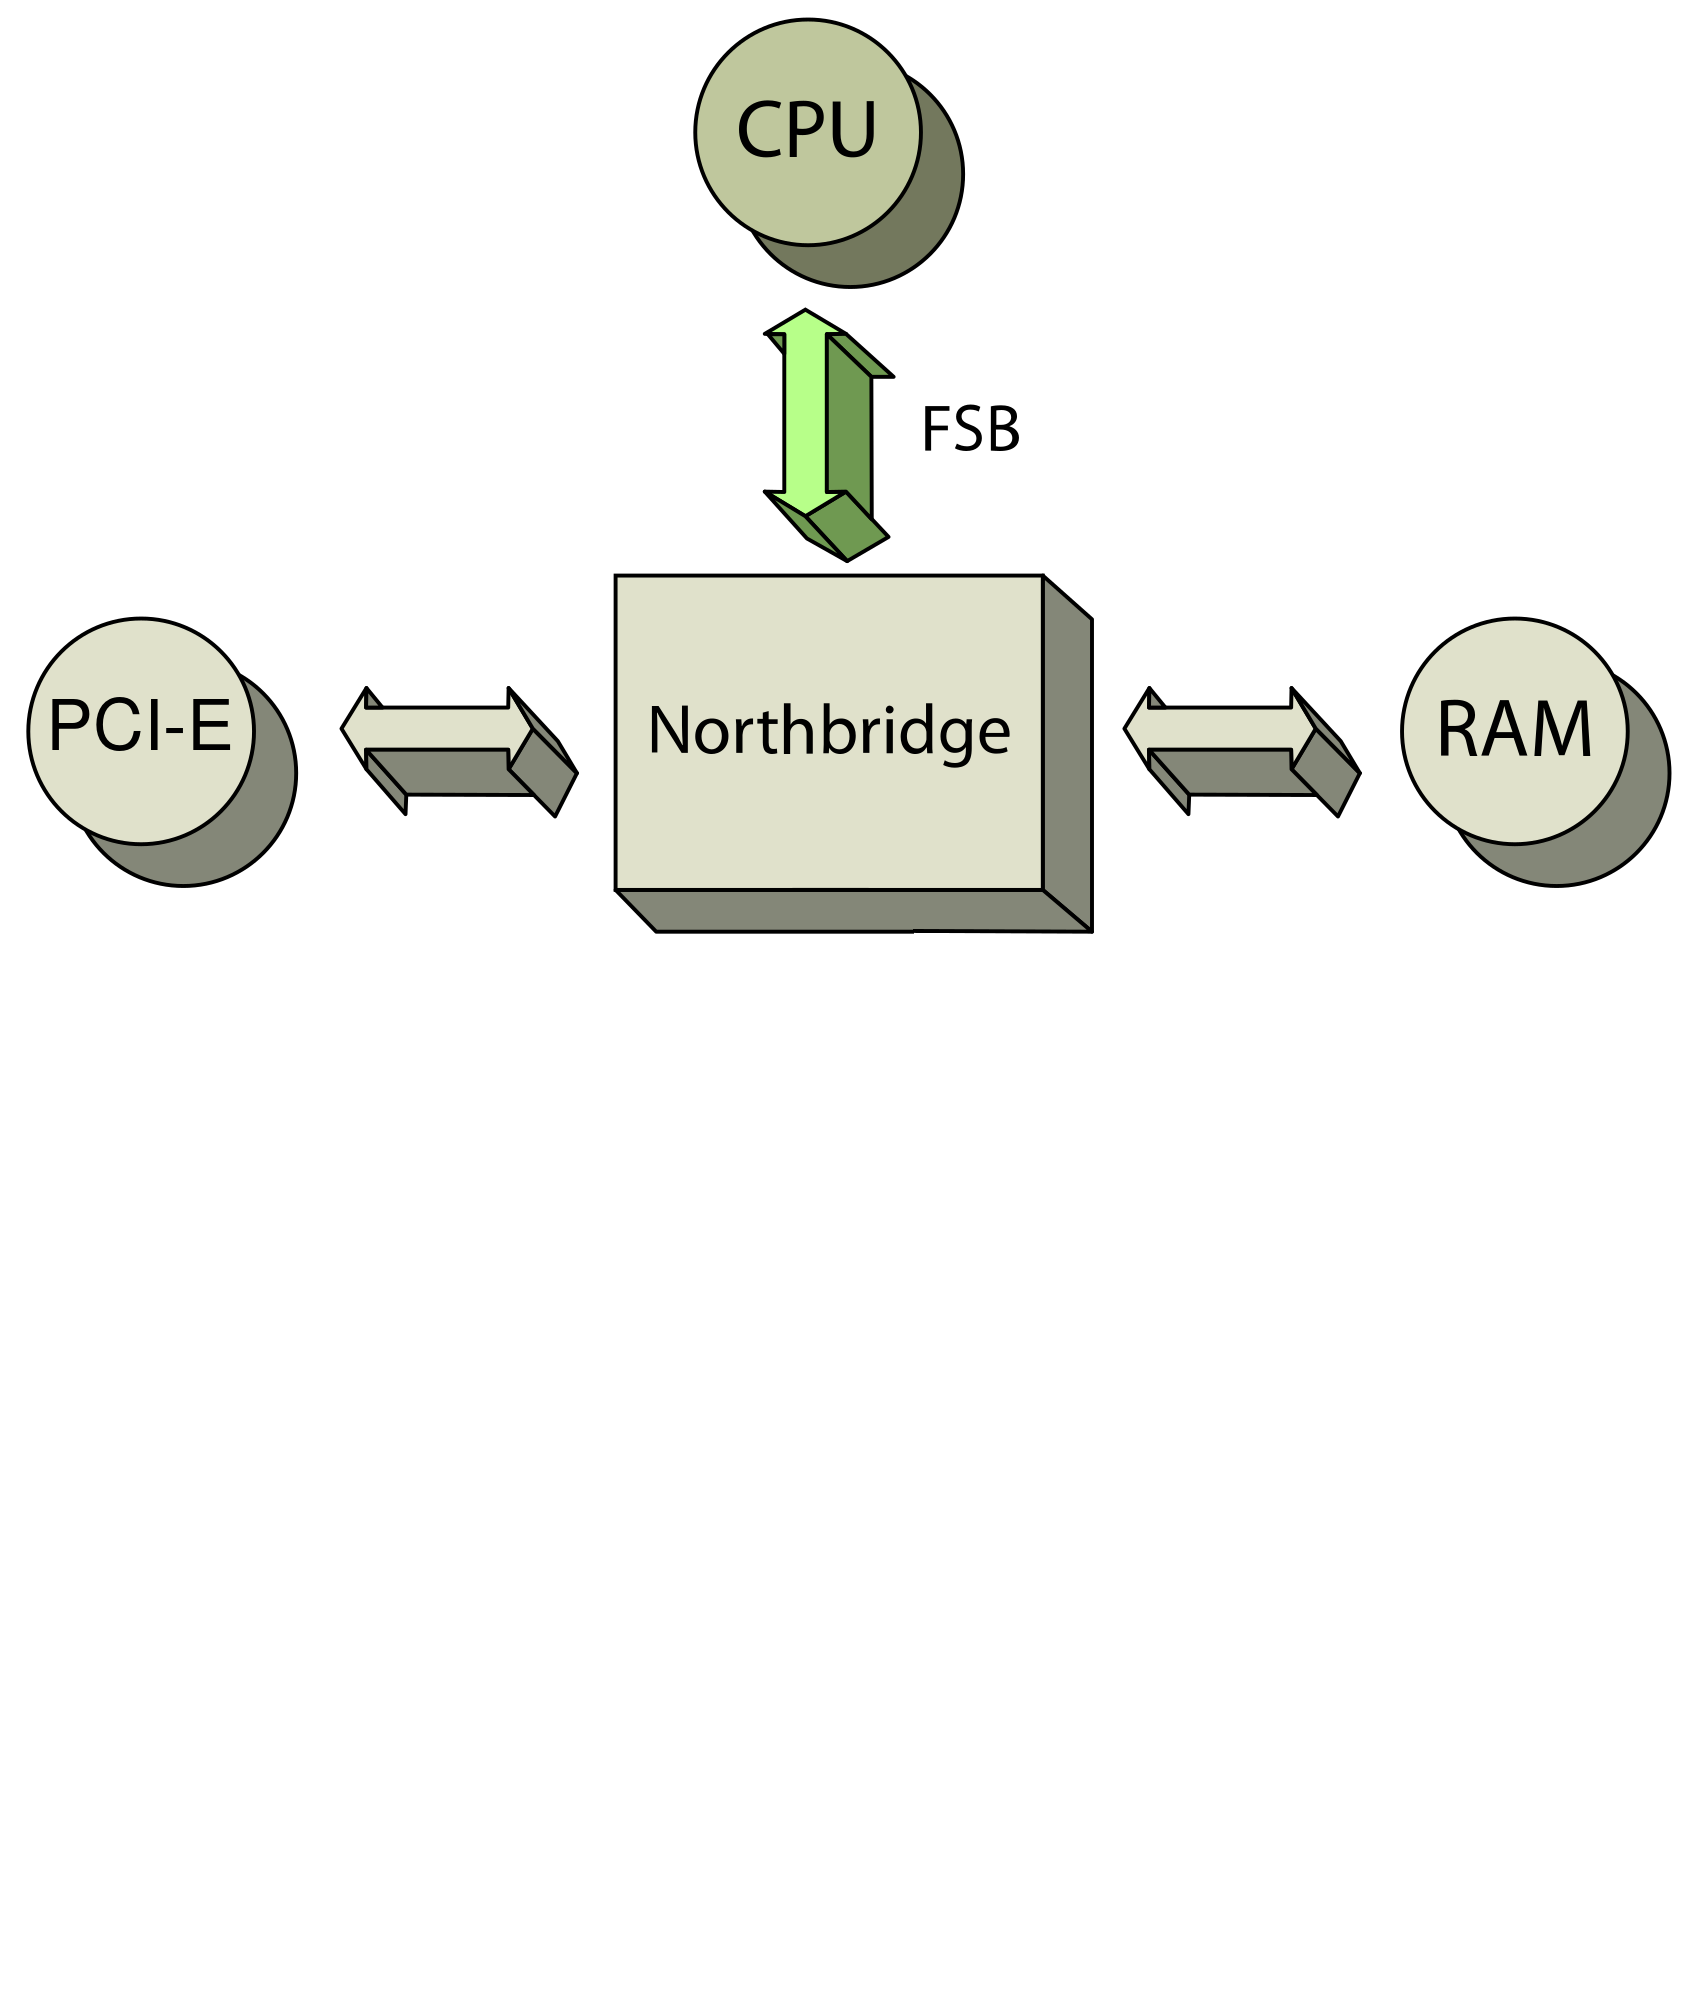
\includegraphics[width=7cm]{architecture5.png}
\end{frame}

% - South Bridge verbunden.
%   - Das ist der Chip der sich um den Datentransfer des langsamen Scheiss kuemmert. 
\begin{frame}[t]
\frametitle{Wie ist ein PC aufgebaut?}
\centering
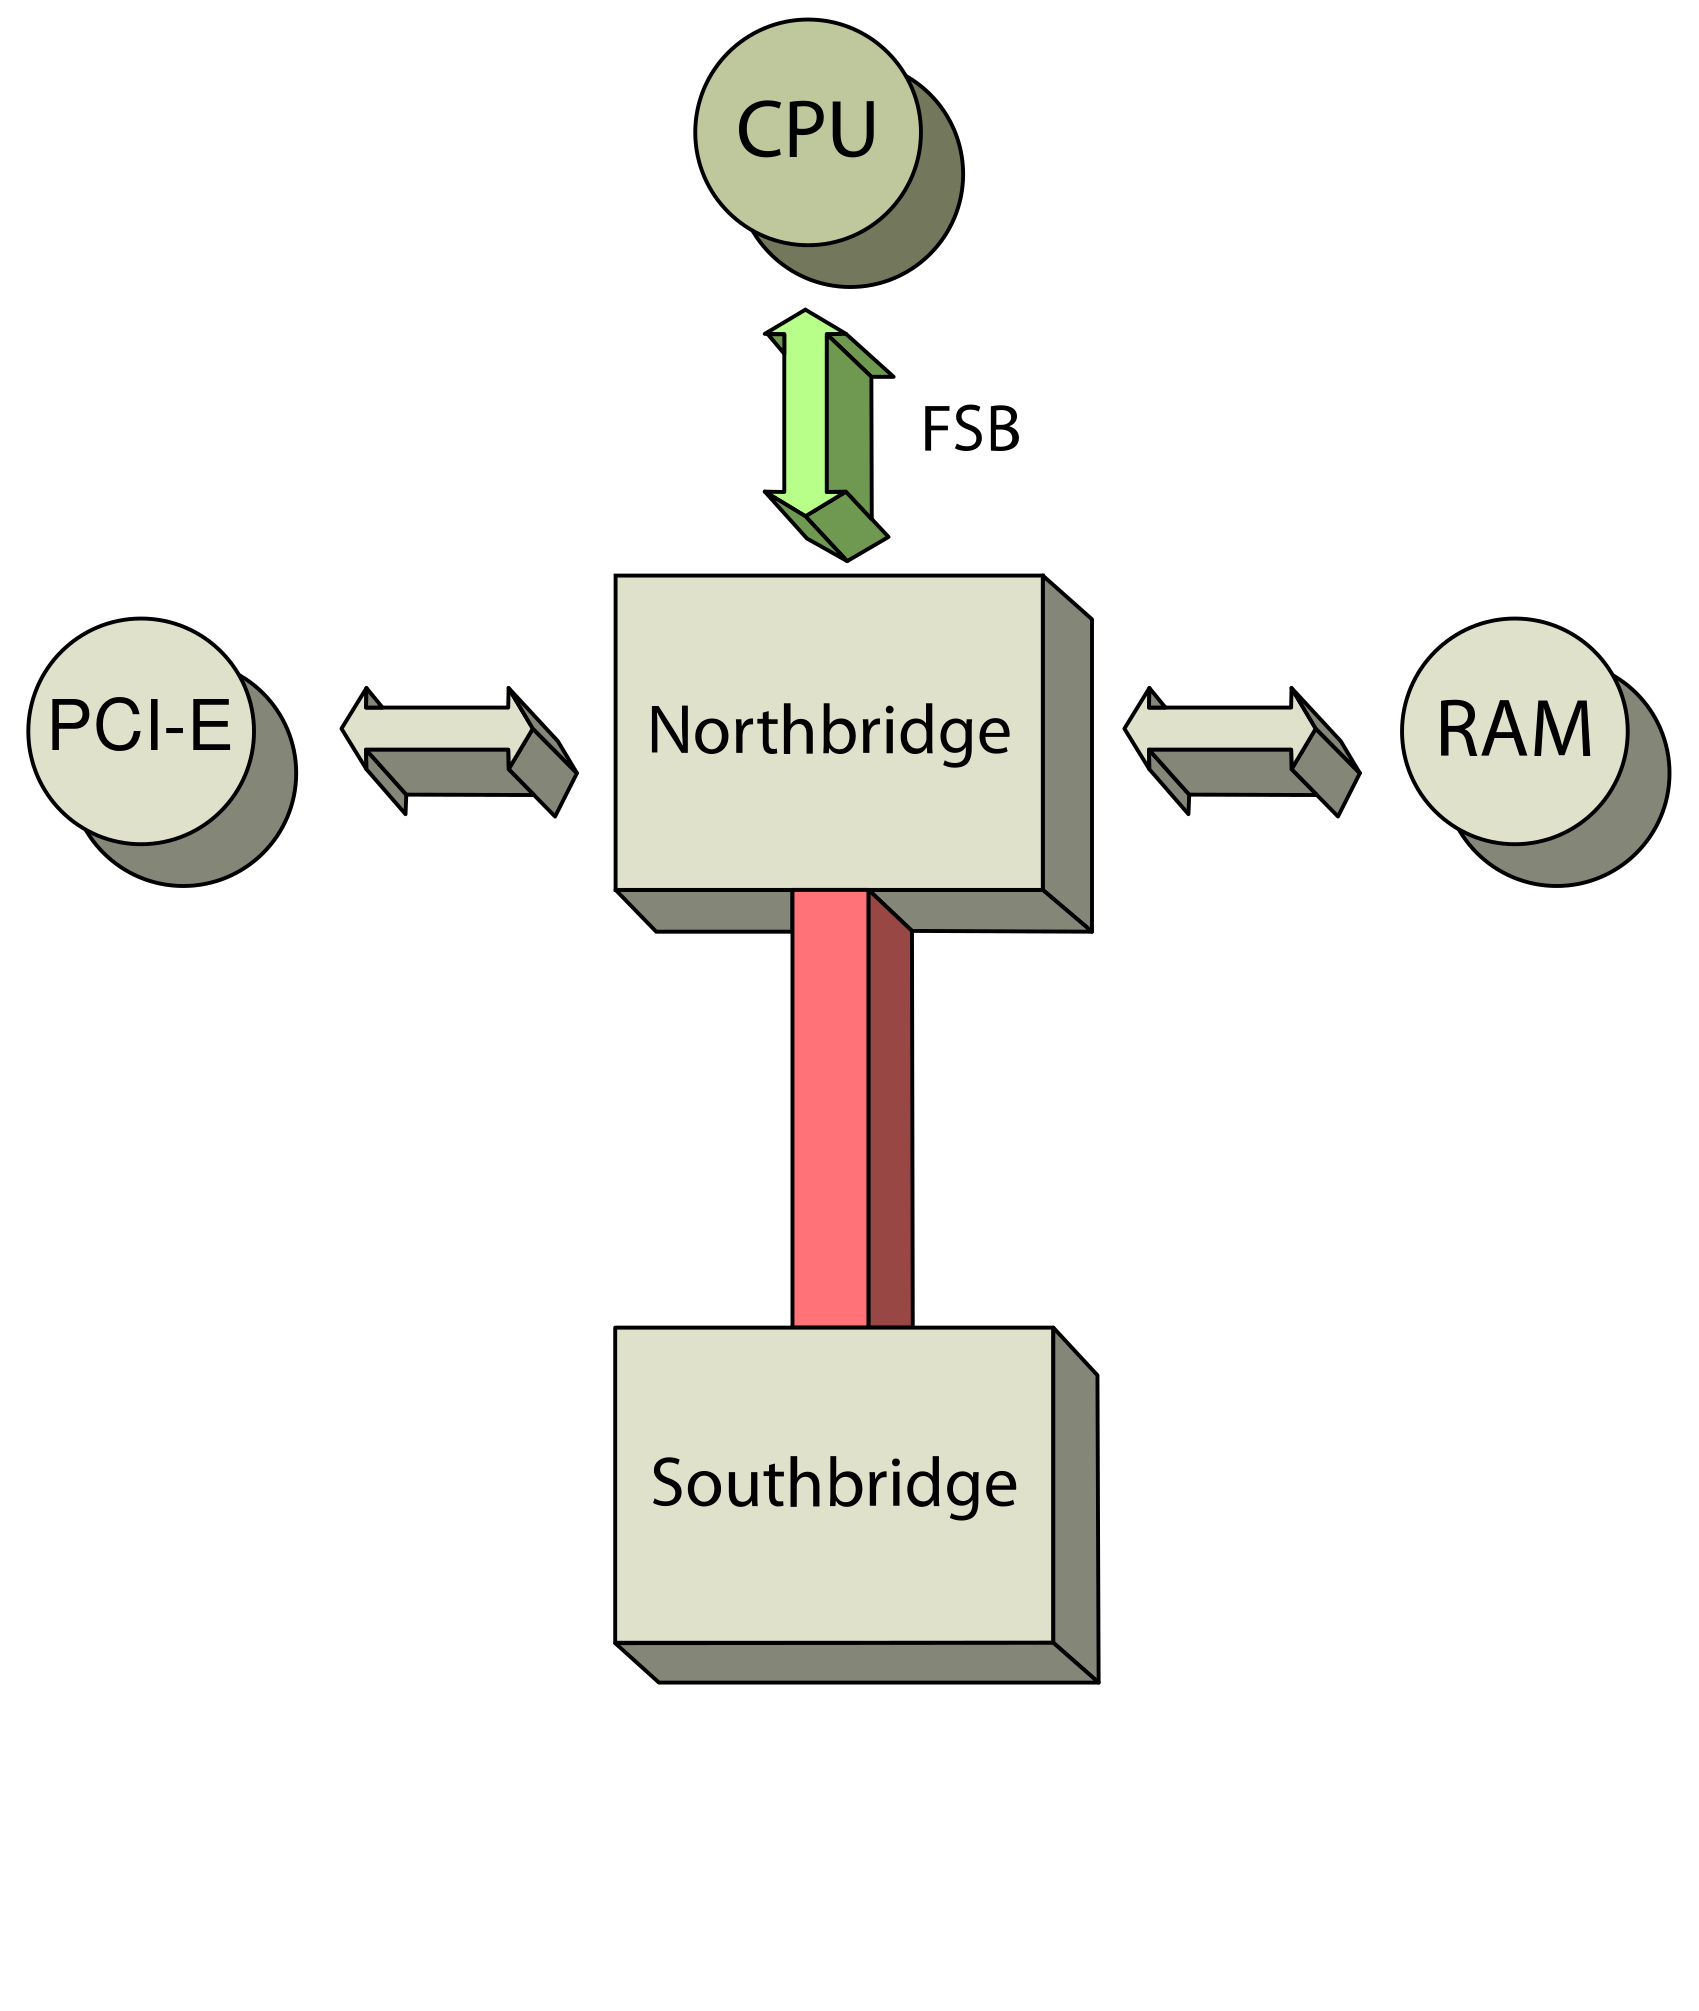
\includegraphics[width=7cm]{architecture6.png}
\end{frame}

% - Die Grafik ist veraltet, das wichtigste sind
%   - USB/USB-C/Thunderbolt
%   - Festplatten: HDDs (Hard Disk Drives) und SSDs (Solid State Drives) via SATA (Serial ATA)
%   - Ethernet und WiFi-Karten
%   - Und anderer alter Kram wie hier IDE (Integrated Drive Electronics) /PATA (Parallel ATA)
%
% - Der Memory alleine waere doch zu langsam und die Register zu klein.
%   Lasst uns nochmal etwas genauer den CPU angucken.
\begin{frame}[t]
\frametitle{Wie ist ein PC aufgebaut?}
\centering
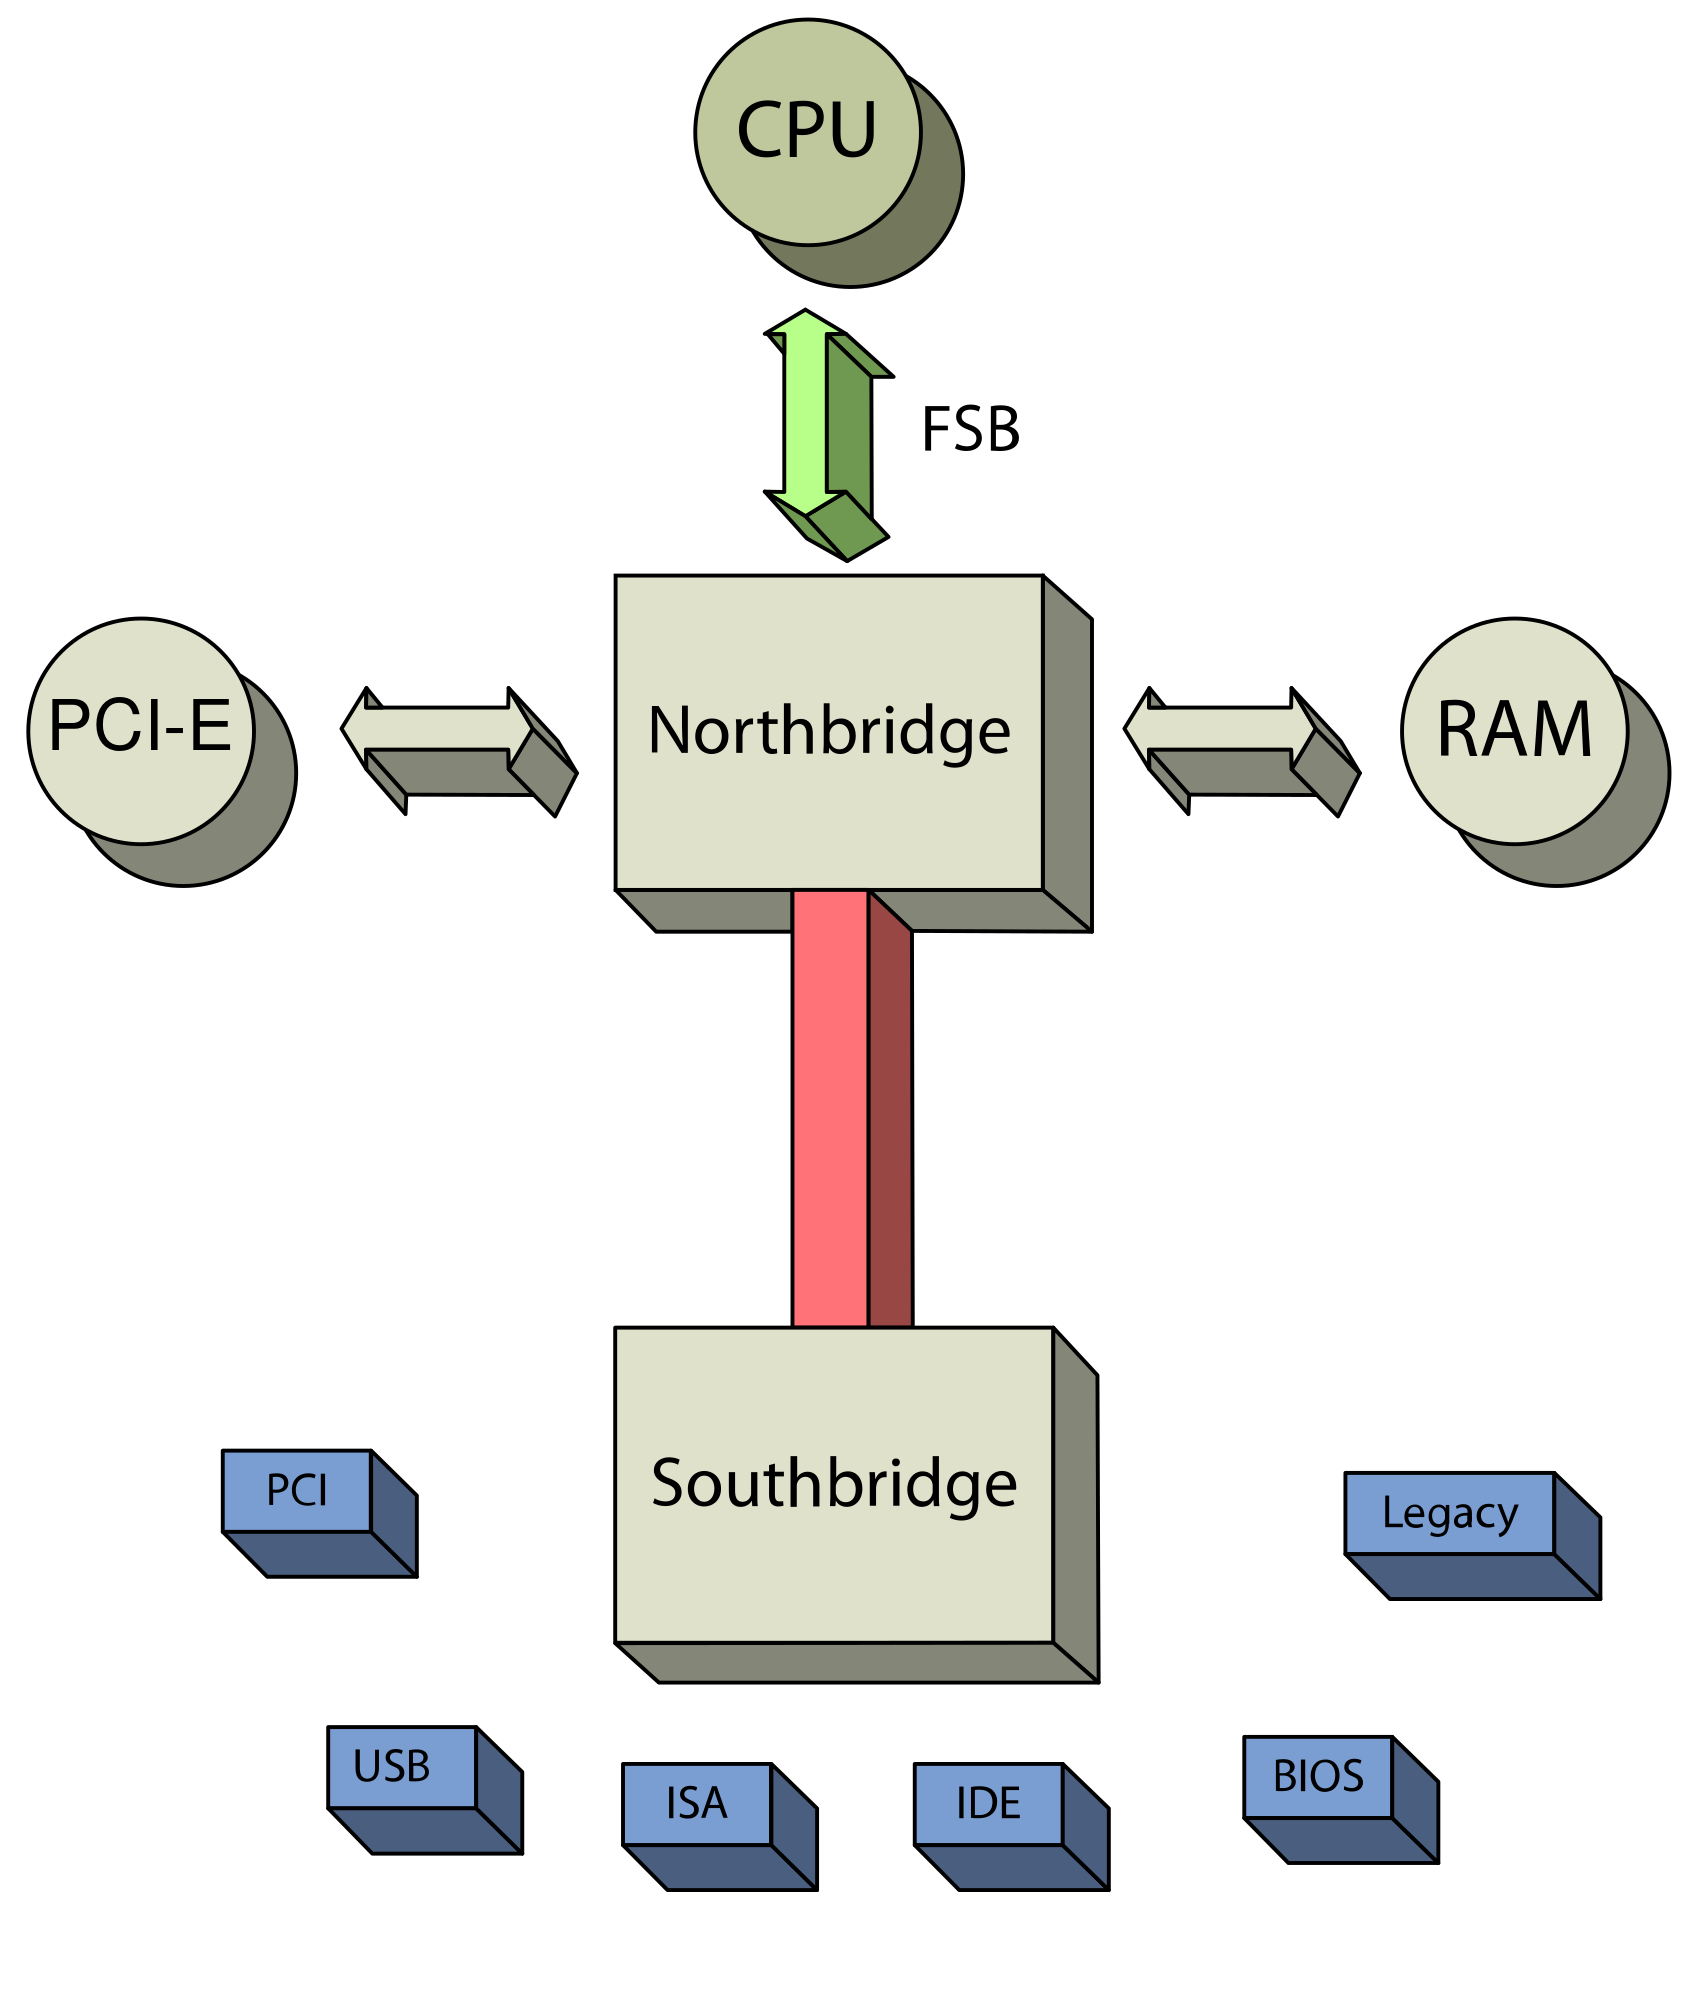
\includegraphics[width=7cm]{architecture7.png}
\end{frame}

% - Ein CPU hat einen Core.
% - Dort ist alles besprochene drin.
% - Ein Core kann mehrere Threads haben.
\begin{frame}[t]
\frametitle{Wie ist ein CPU aufgebaut?}
\centering
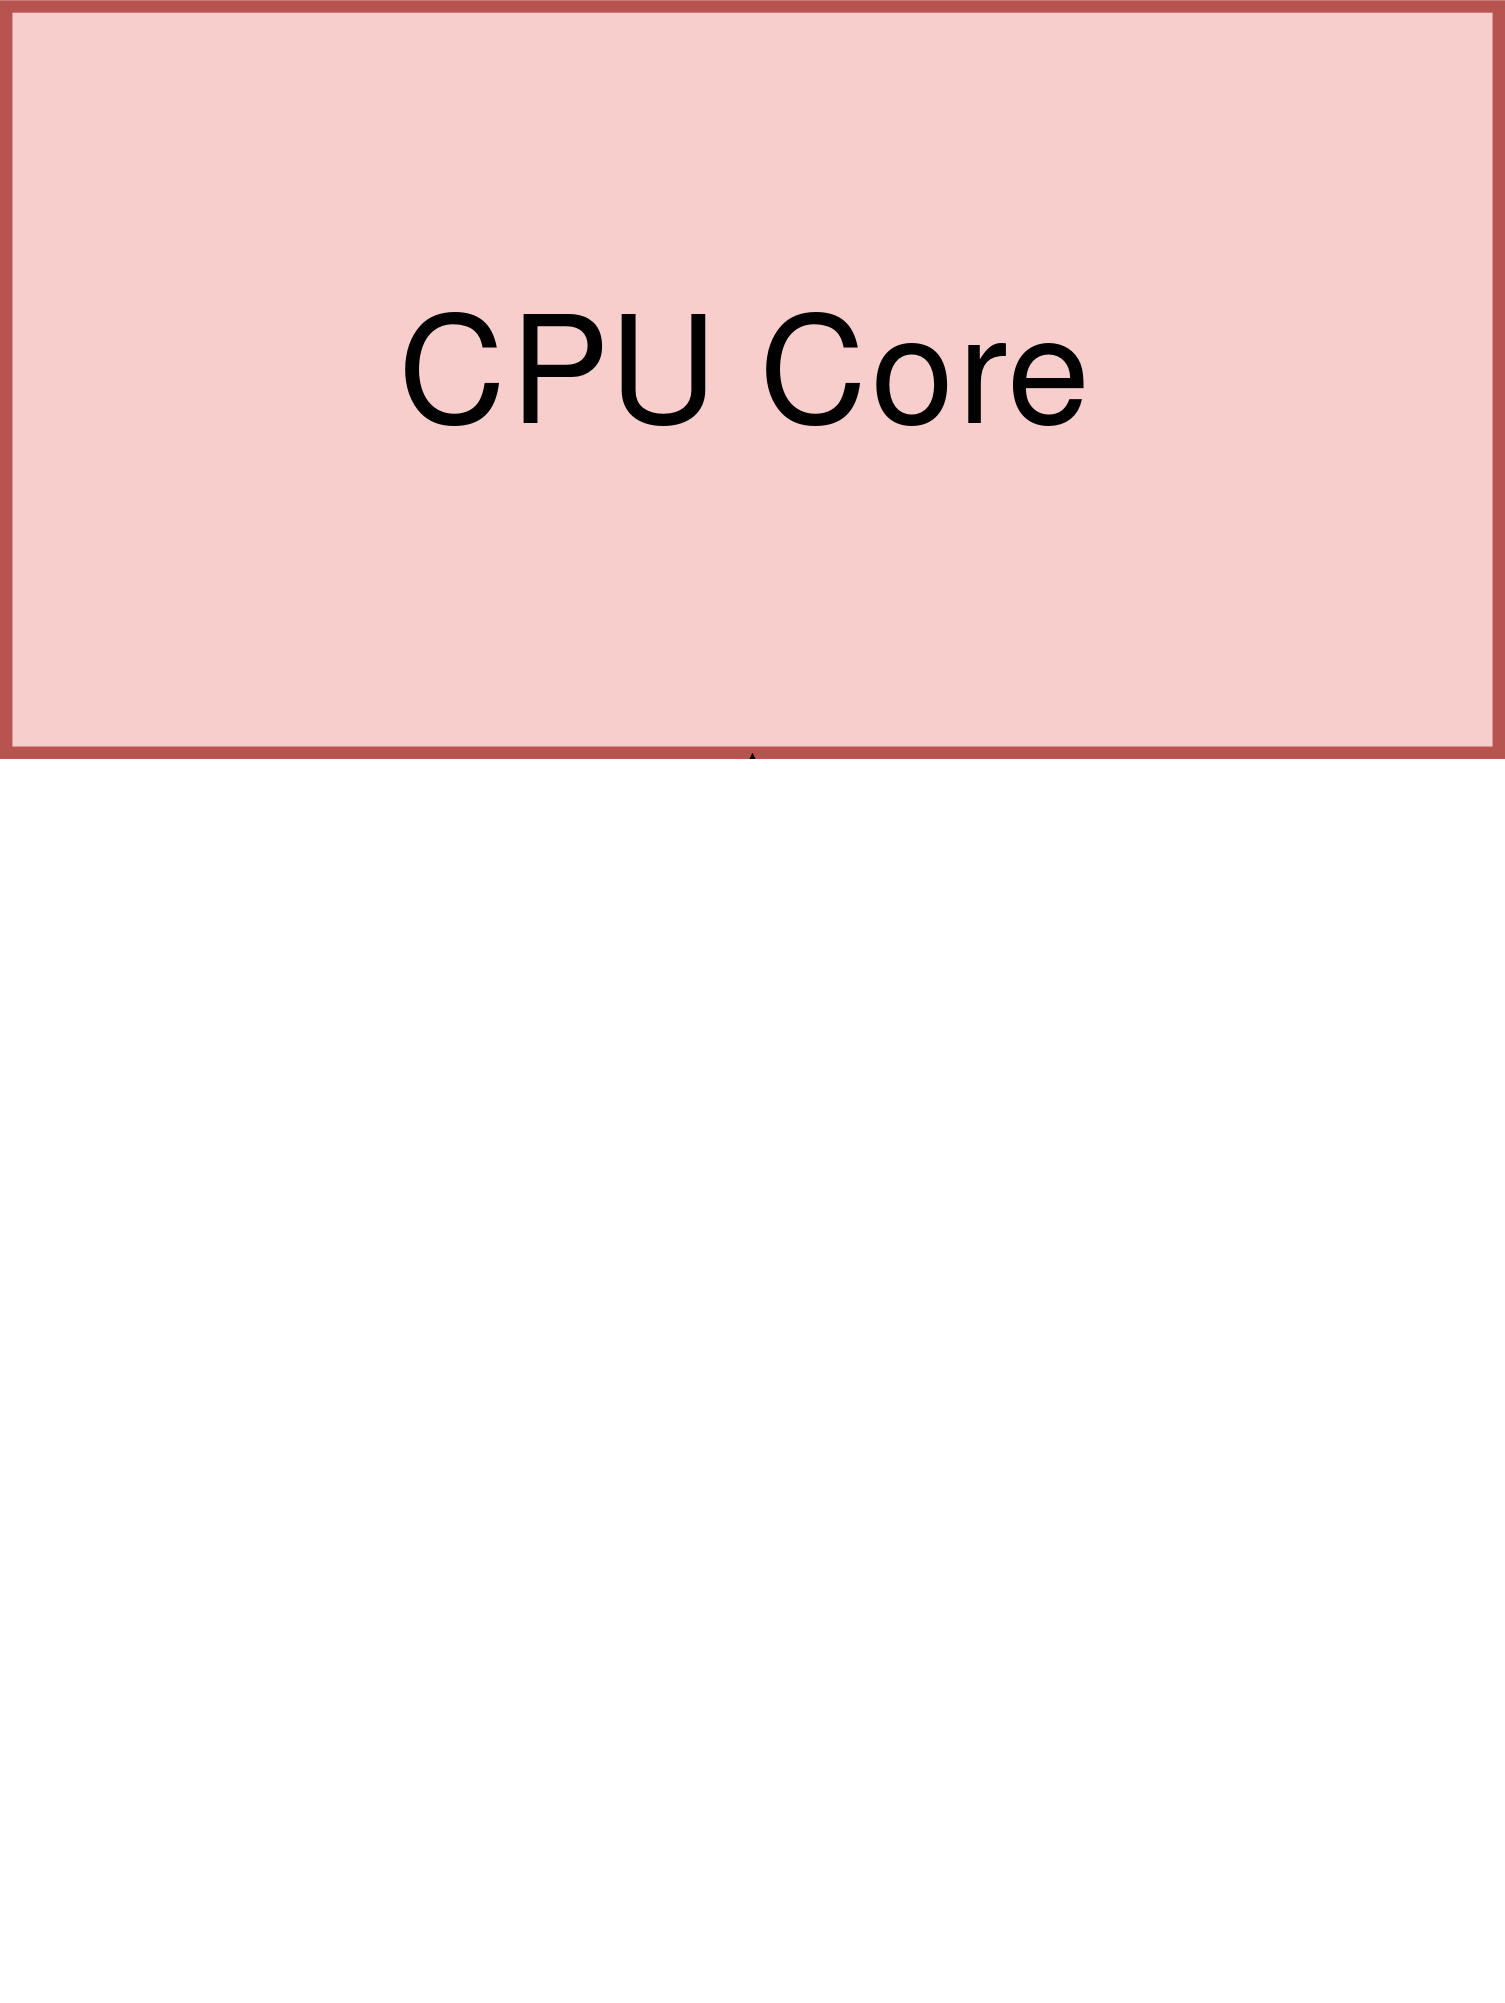
\includegraphics[height=5cm]{cpu1.PNG}
\end{frame}

% - Ein Core hat einen Level 1 Cache.
% - (Ein Cache ist ein Zwischenspeicher, wo man Sachen speichert die man gerade genutzt hat,
%   falls man sie in der nahen Zukunft wieder braucht)
% - Dieser ist SEHR schnell
% - Bei mir hier 128KB gross. Unbezahlbar teuer, deswegen nur so klein.
% - Dieser wird fuer Sachen genutzt mit denen der Prozessor zuletzt gearbeitet hat
%   - Falls man auf die Variablen wieder schnell zugreifen muss
%   - Wie zum Beispiel ein i bei einer for loop
%   - oder ein kleines Objekt was man dauerhaft veraendet
%
% - Mehrere Threads auf einen Core teilen sich den selben L1 Cache
%
% - Wobei, das war nur die halbe Wahrheit
\begin{frame}[t]
\frametitle{Wie ist ein CPU aufgebaut?}
\centering
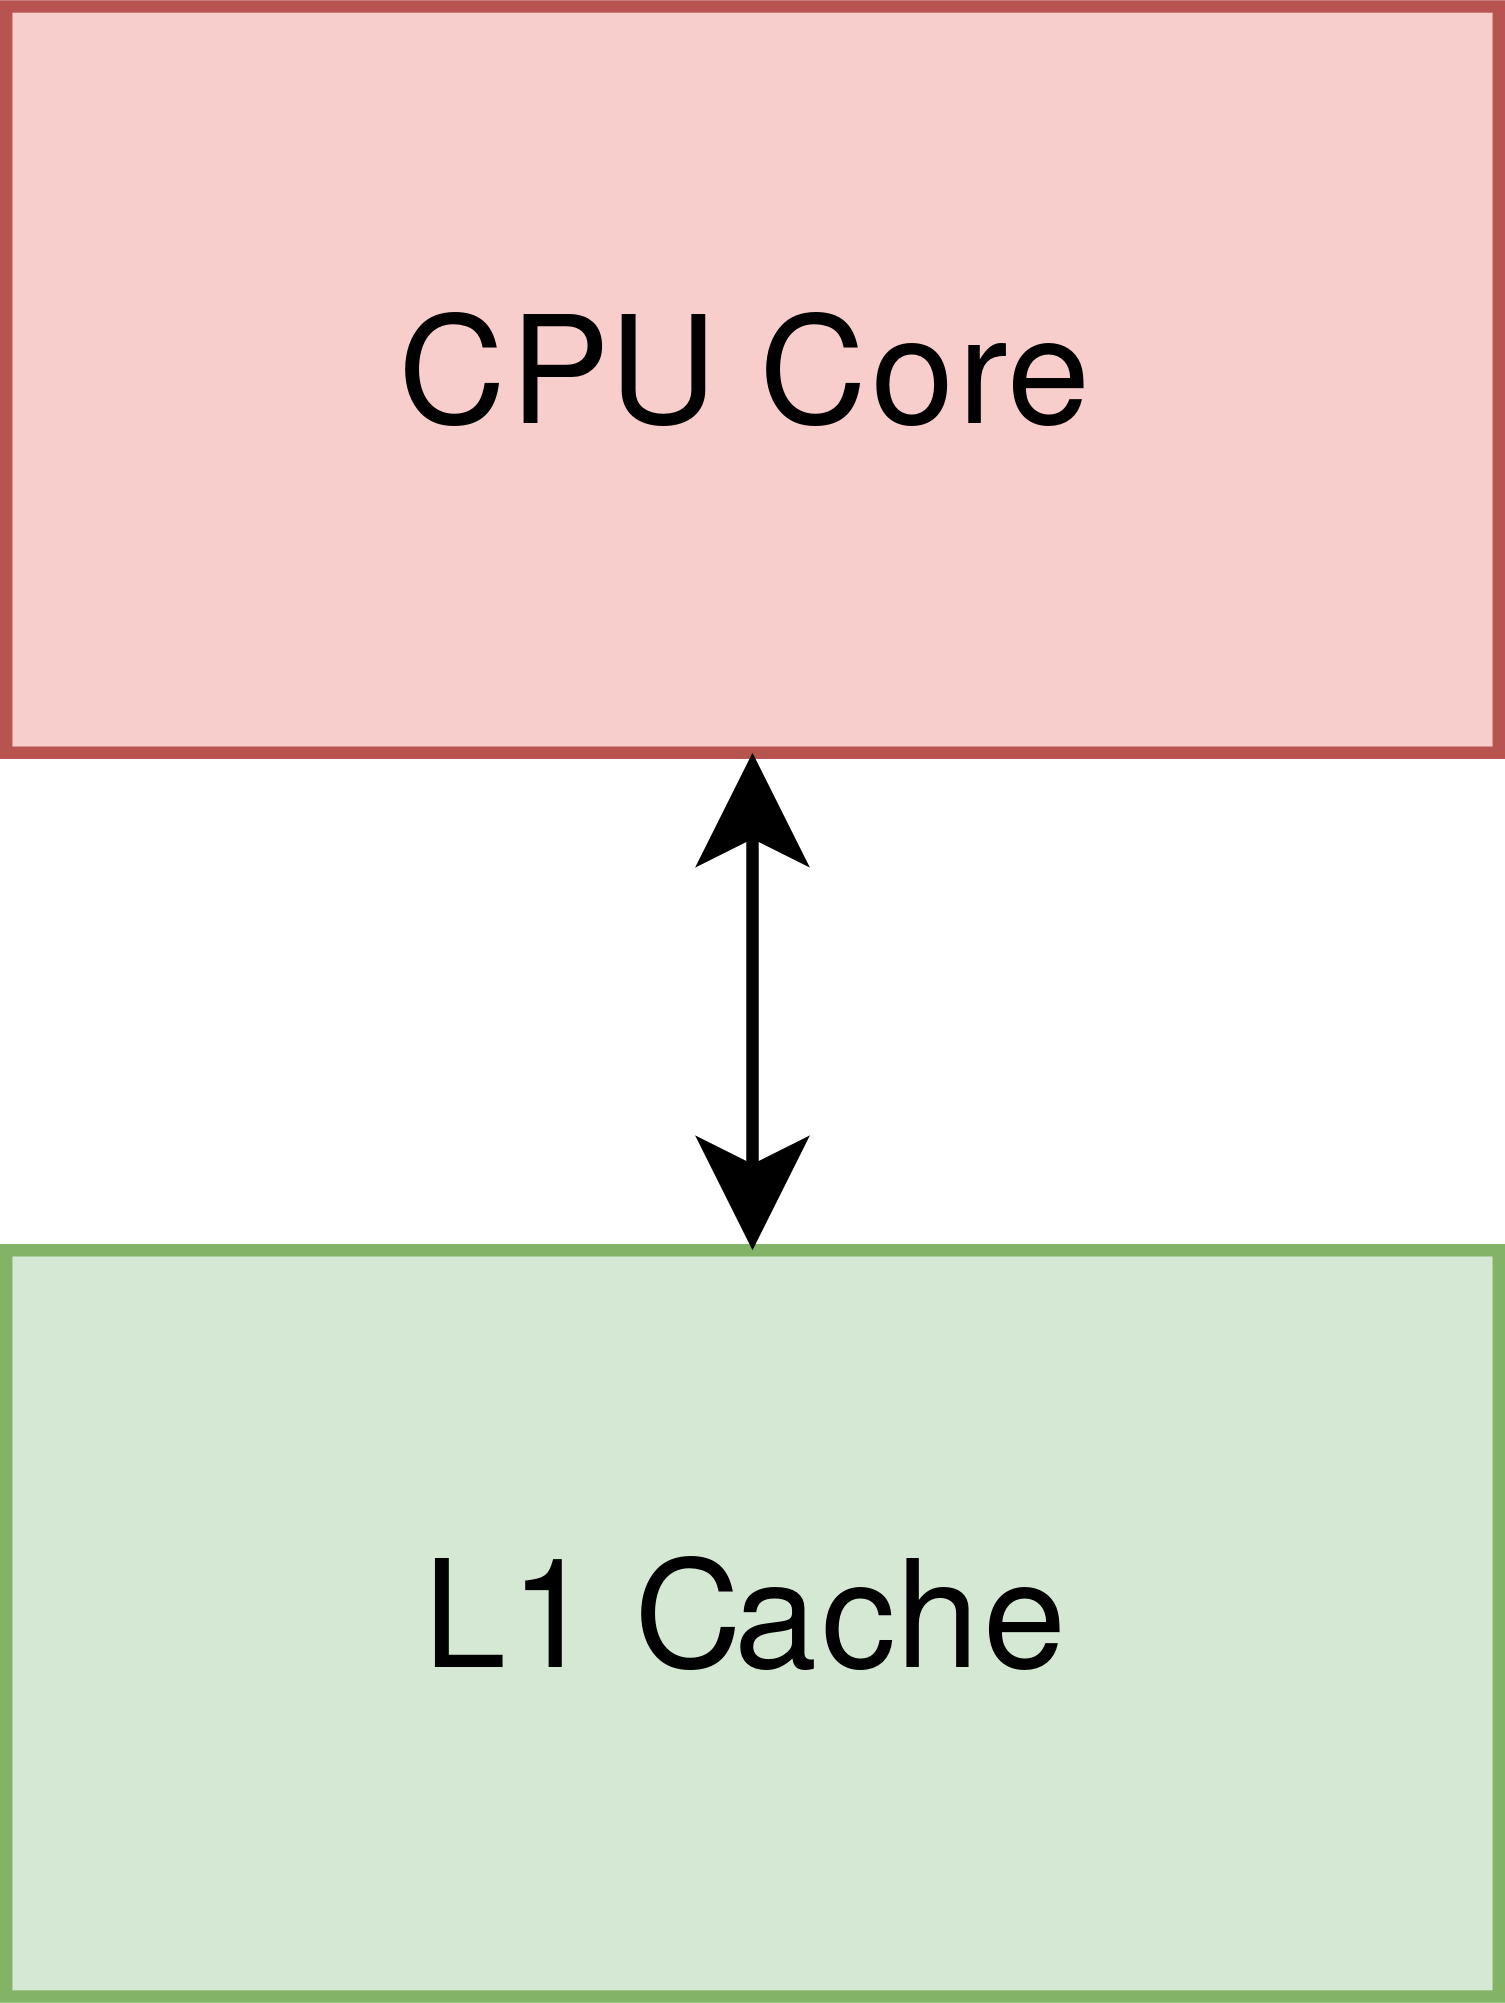
\includegraphics[height=5cm]{CPU2.PNG}
\end{frame}

% - Eigentlich gibt es 2 Level 1 Caches.
% - Einen fuer Instruktionen (L1i) (das Programm selbst) und einen fuer Daten (L1d) (Variablen und so)
% - Sprich bei mir jeweils 64 KB
% - Diese Unterteilung kommt dadurch, dass
%   - Sie andere raeumliche Eigenschaften haben.
%     Instruktionen sind meist hintereinander,
%     Daten, gerade im Heap, oft verteilt.
%   - Man brauch andere Metainformationen.
%     Instruktionen sind zB read-only
%     Auch wenn Haskeller diesen Fakt hassen, Daten darf man veraendern.
%
% - Jedoch
\begin{frame}[t]
\frametitle{Wie ist ein CPU aufgebaut?}
\centering
\includegraphics[height=5cm]{cpu3.png}
\end{frame}

% - Hat ein moderner PC mehrere Cores. Meiner hat zB 4.
% 
% - Alle Cores teilen sich
\begin{frame}[t]
\frametitle{Wie ist ein CPU aufgebaut?}
\centering
\centerline{\includegraphics[width=12cm]{cpu4.png}}
\end{frame}

% - Einen Level 2 cache.
% - Dieser ist langsamer als ein L1 cache, dafuer aber viel groesser.
%   - Meine L1 caches sind je 64KB
%   - Mein L2 cache ist 1MB (Sprich 16x die groesse eines L1 caches)
%
% UND
\begin{frame}[t]
\frametitle{Wie ist ein CPU aufgebaut?}
\centering
\centerline{\includegraphics[width=12cm]{cpu5.png}}
\end{frame}

% - Es gibt einen L3 cache.
% - Der ist noch langsamer, und noch groesser.
% - Bei mir 8MB, sprich 8x L2, und 128x mein L1 cache.
% <PAUSE>
\begin{frame}[t]
\frametitle{Wie ist ein CPU aufgebaut?}
\centering
\centerline{\includegraphics[width=12cm]{cpu6.png}}
\end{frame}

\begin{frame}
\centering
\Huge
    Was passiert, wenn man auf eine Variable zugreift?
\end{frame}

% TODO: ERWAEHNEN WARUM DER L1i nicht da ist
\begin{frame}{Was passiert, wenn man auf eine Variable zugreift?}
\vspace*{0.5cm}
\centerline{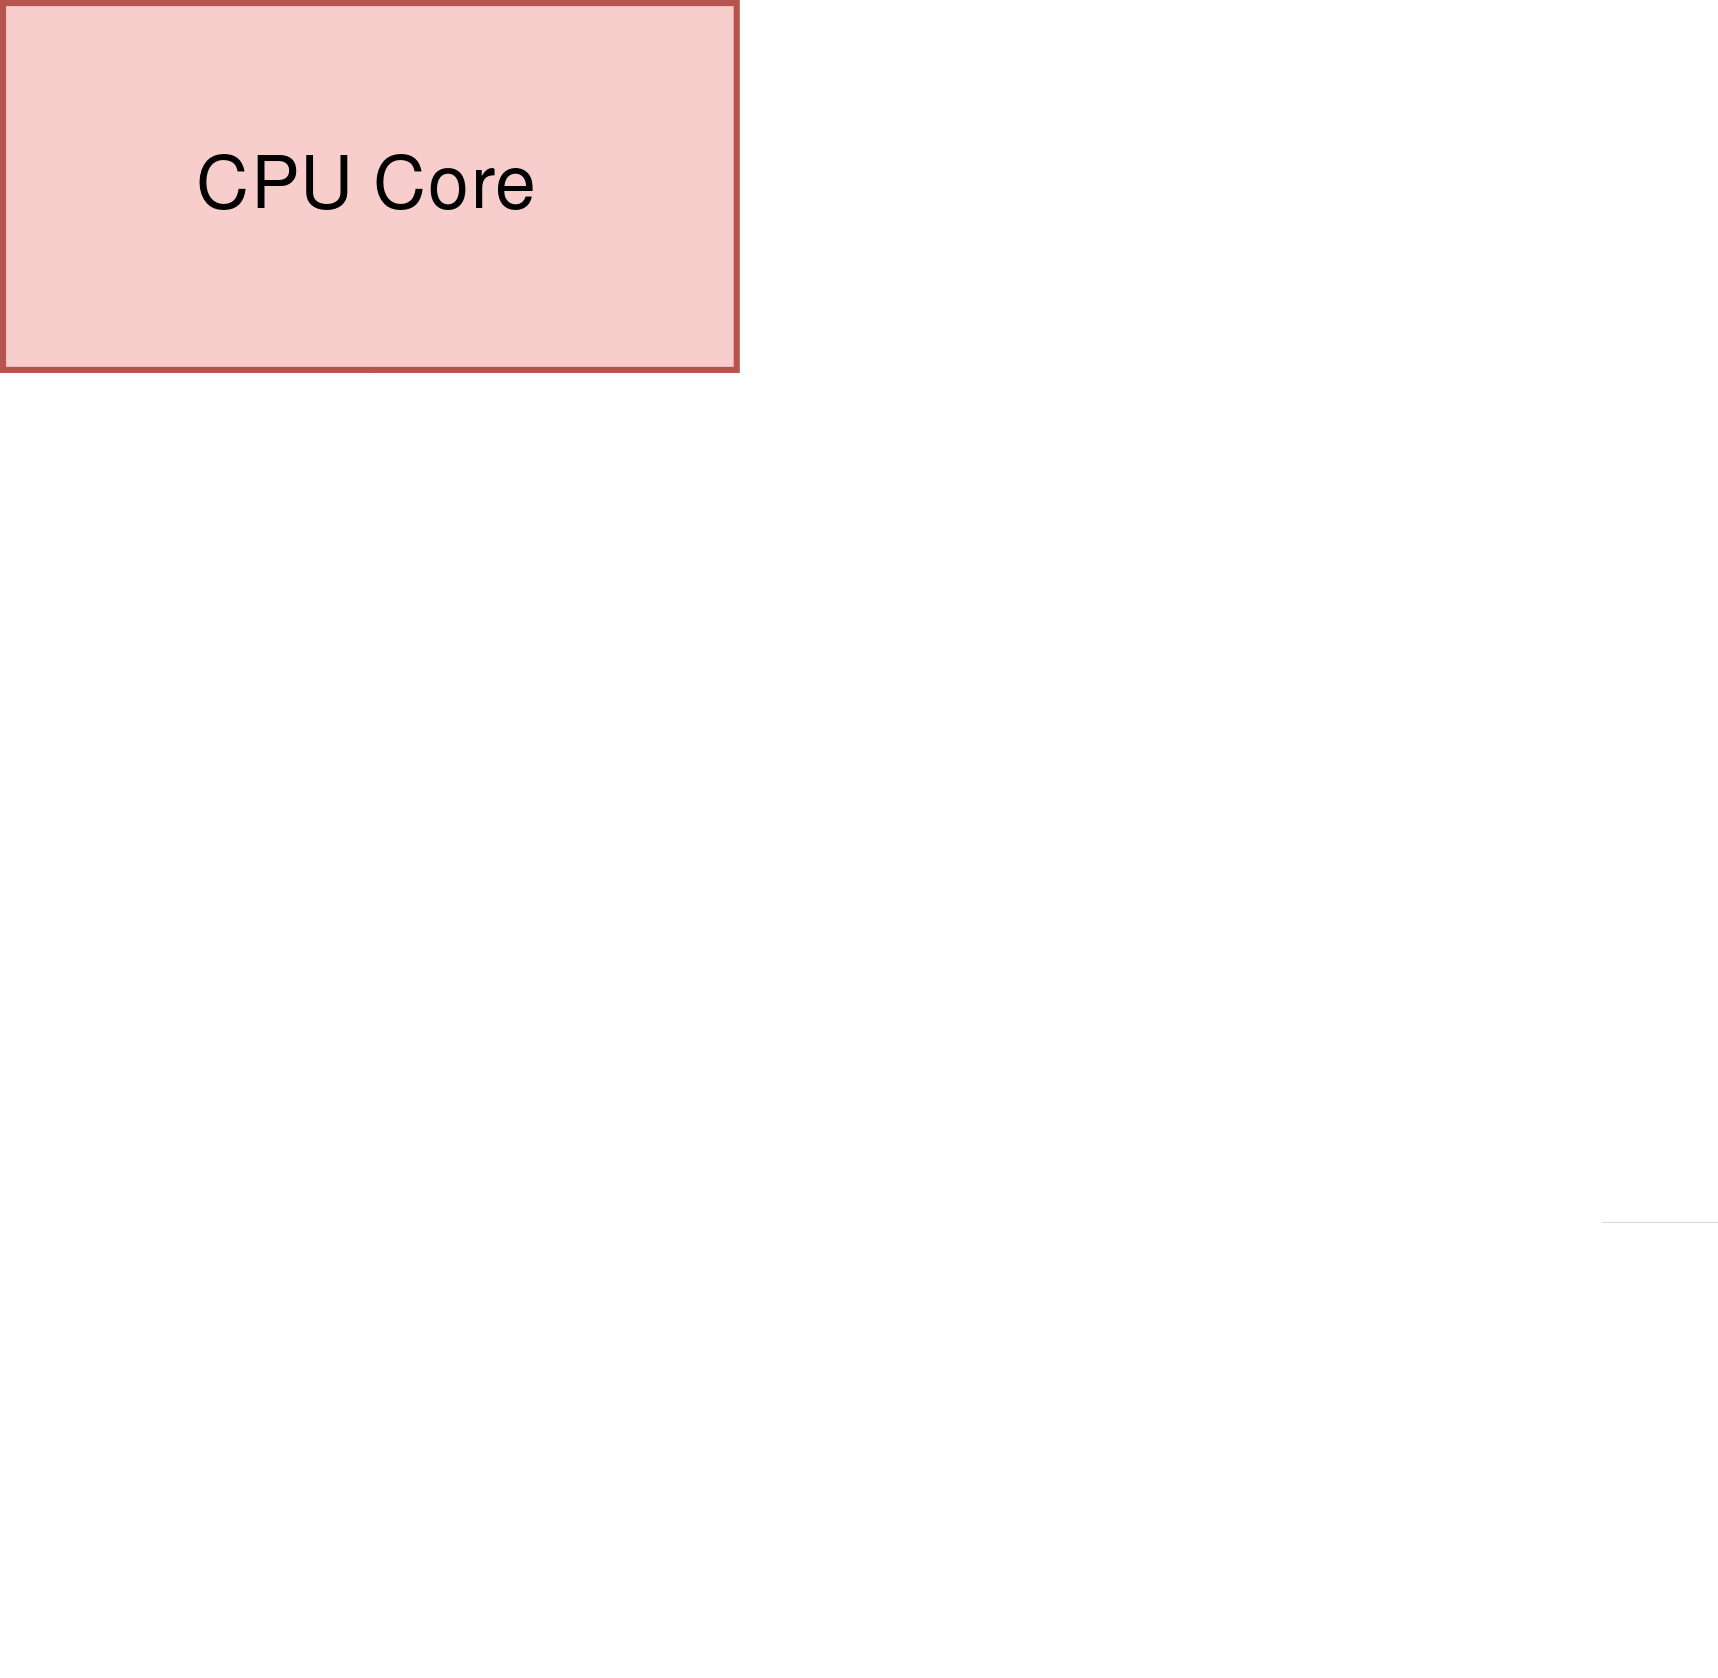
\includegraphics[height=8cm]{trace1.png}}
\end{frame}

% Da wir nur auf Variablen zugreifen, geht es nur durch den L1 data cache, nicht durch den
% L1 instruction cache.
\begin{frame}{Was passiert, wenn man auf eine Variable zugreift?}
\vspace*{0.5cm}
\centerline{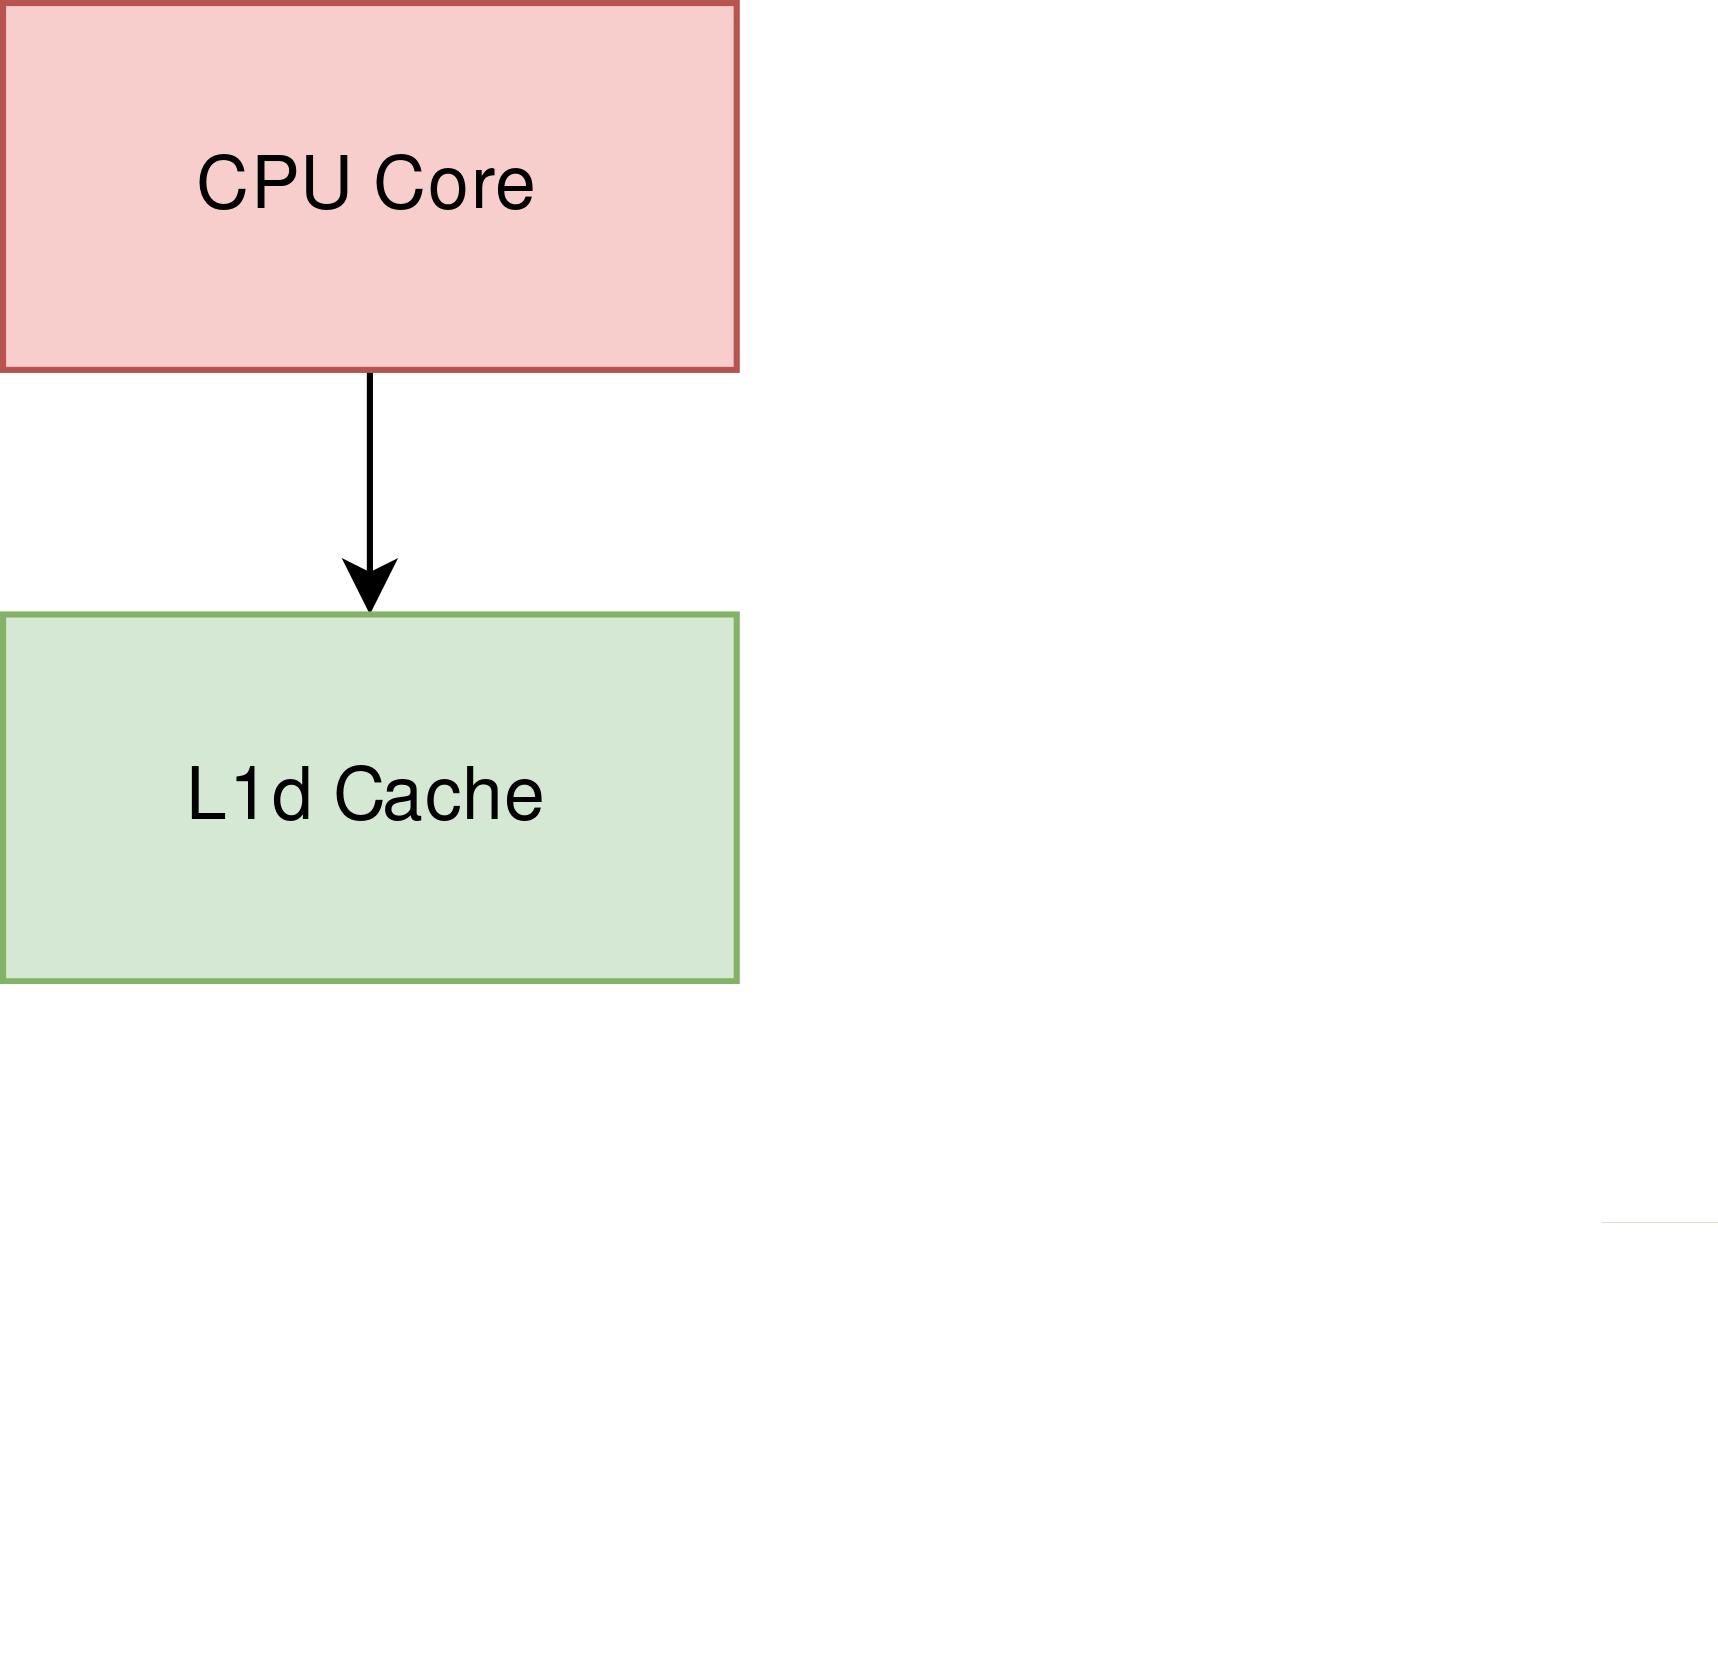
\includegraphics[height=8cm]{trace2.png}}
\end{frame}

\begin{frame}{Was passiert, wenn man auf eine Variable zugreift?}
\vspace*{0.5cm}
\centerline{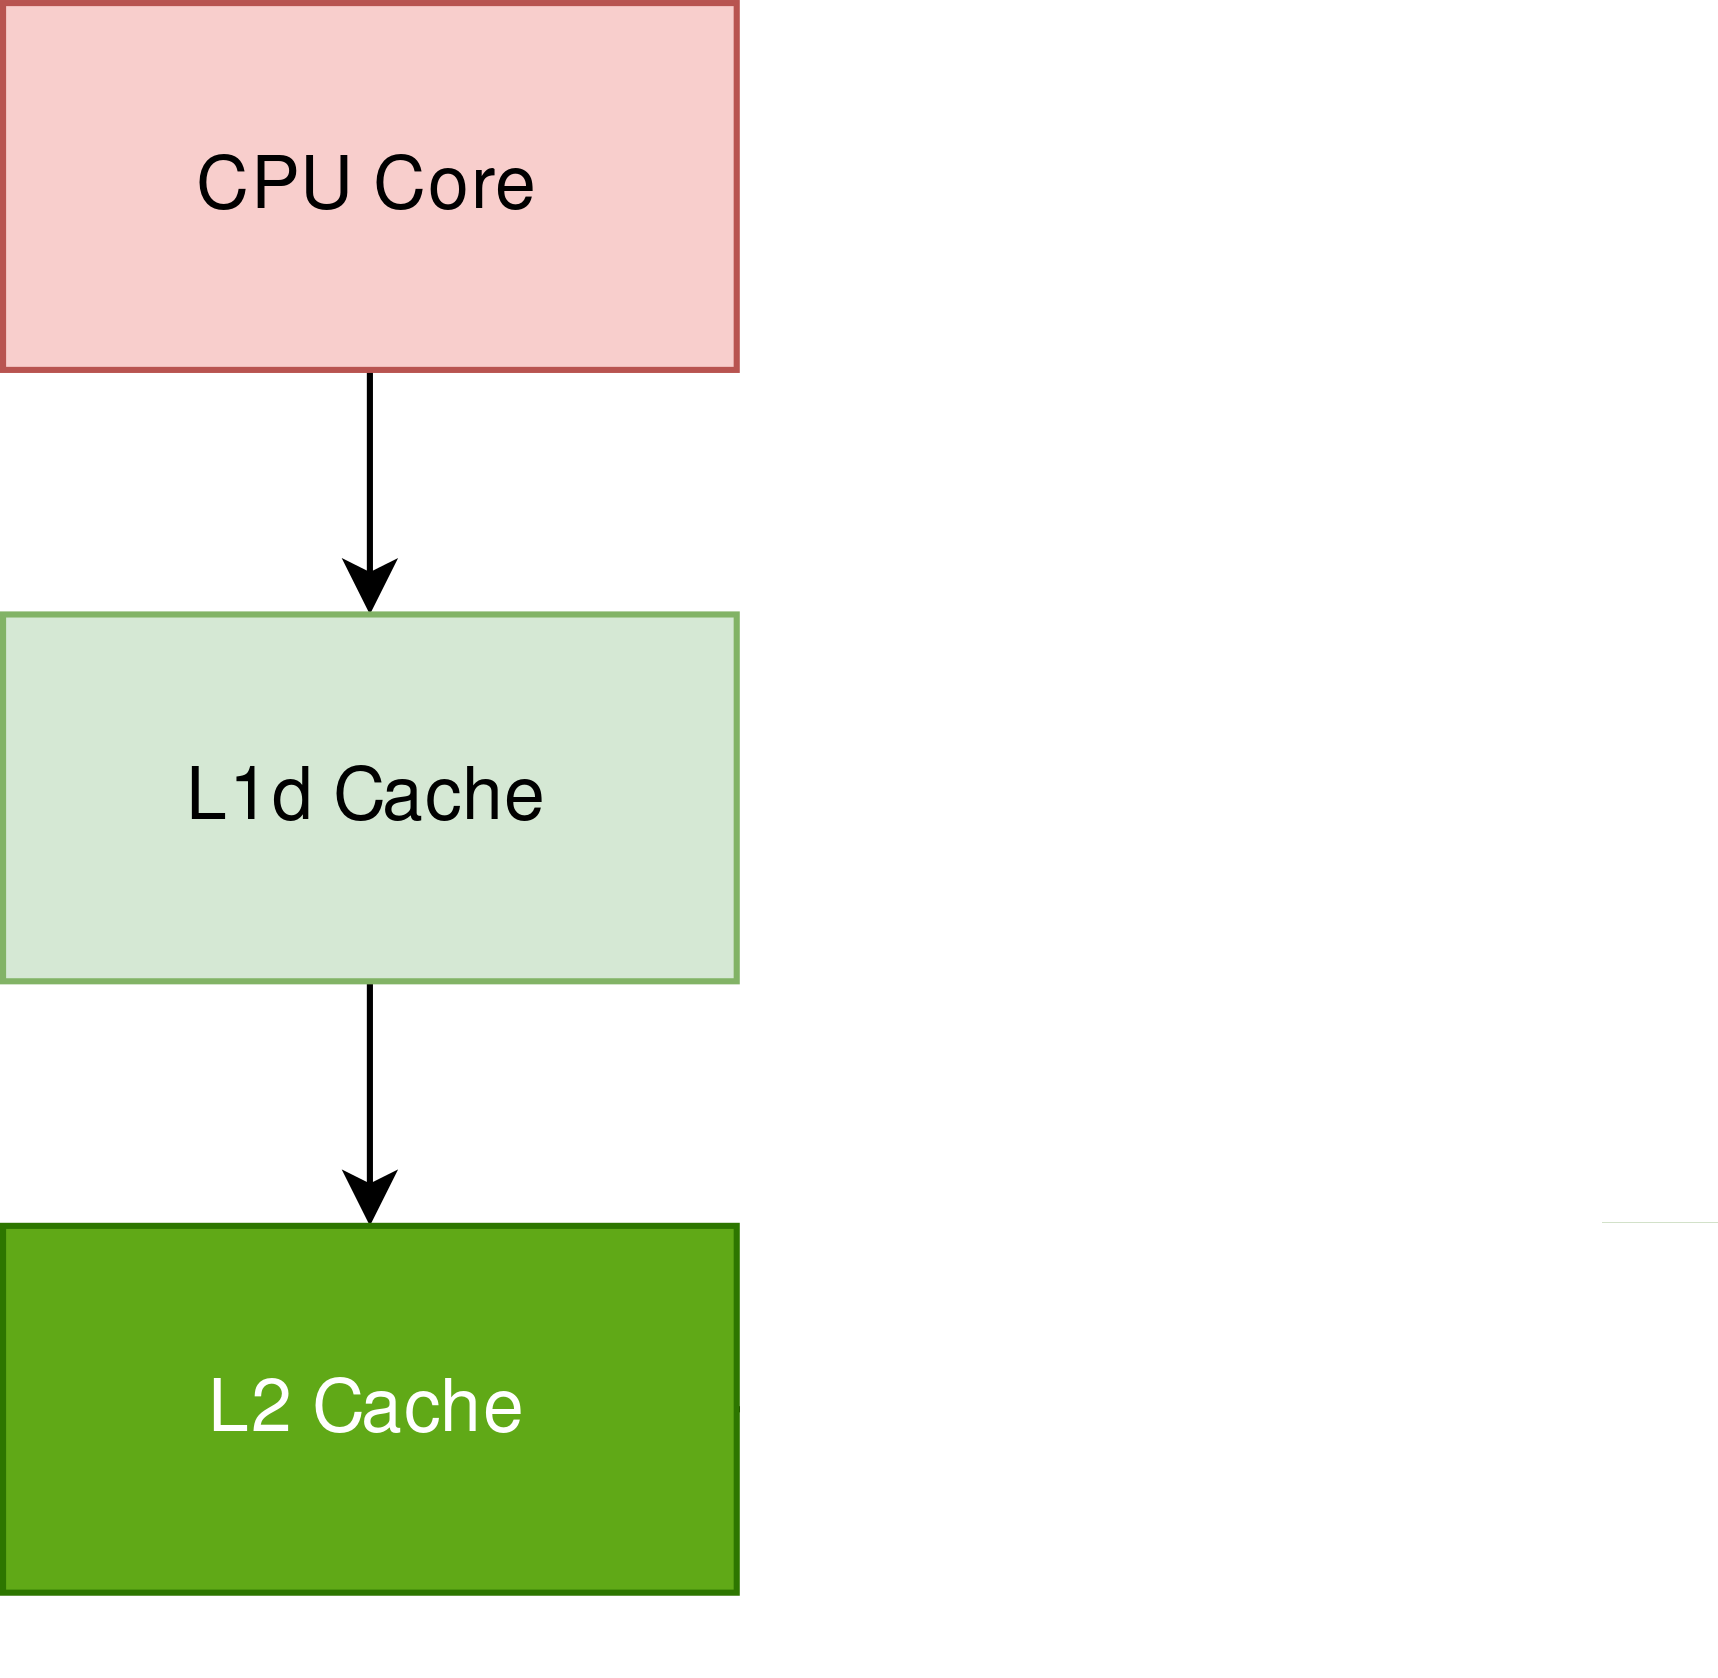
\includegraphics[height=8cm]{trace3.png}}
\end{frame}

\begin{frame}{Was passiert, wenn man auf eine Variable zugreift?}
\vspace*{0.5cm}
\centerline{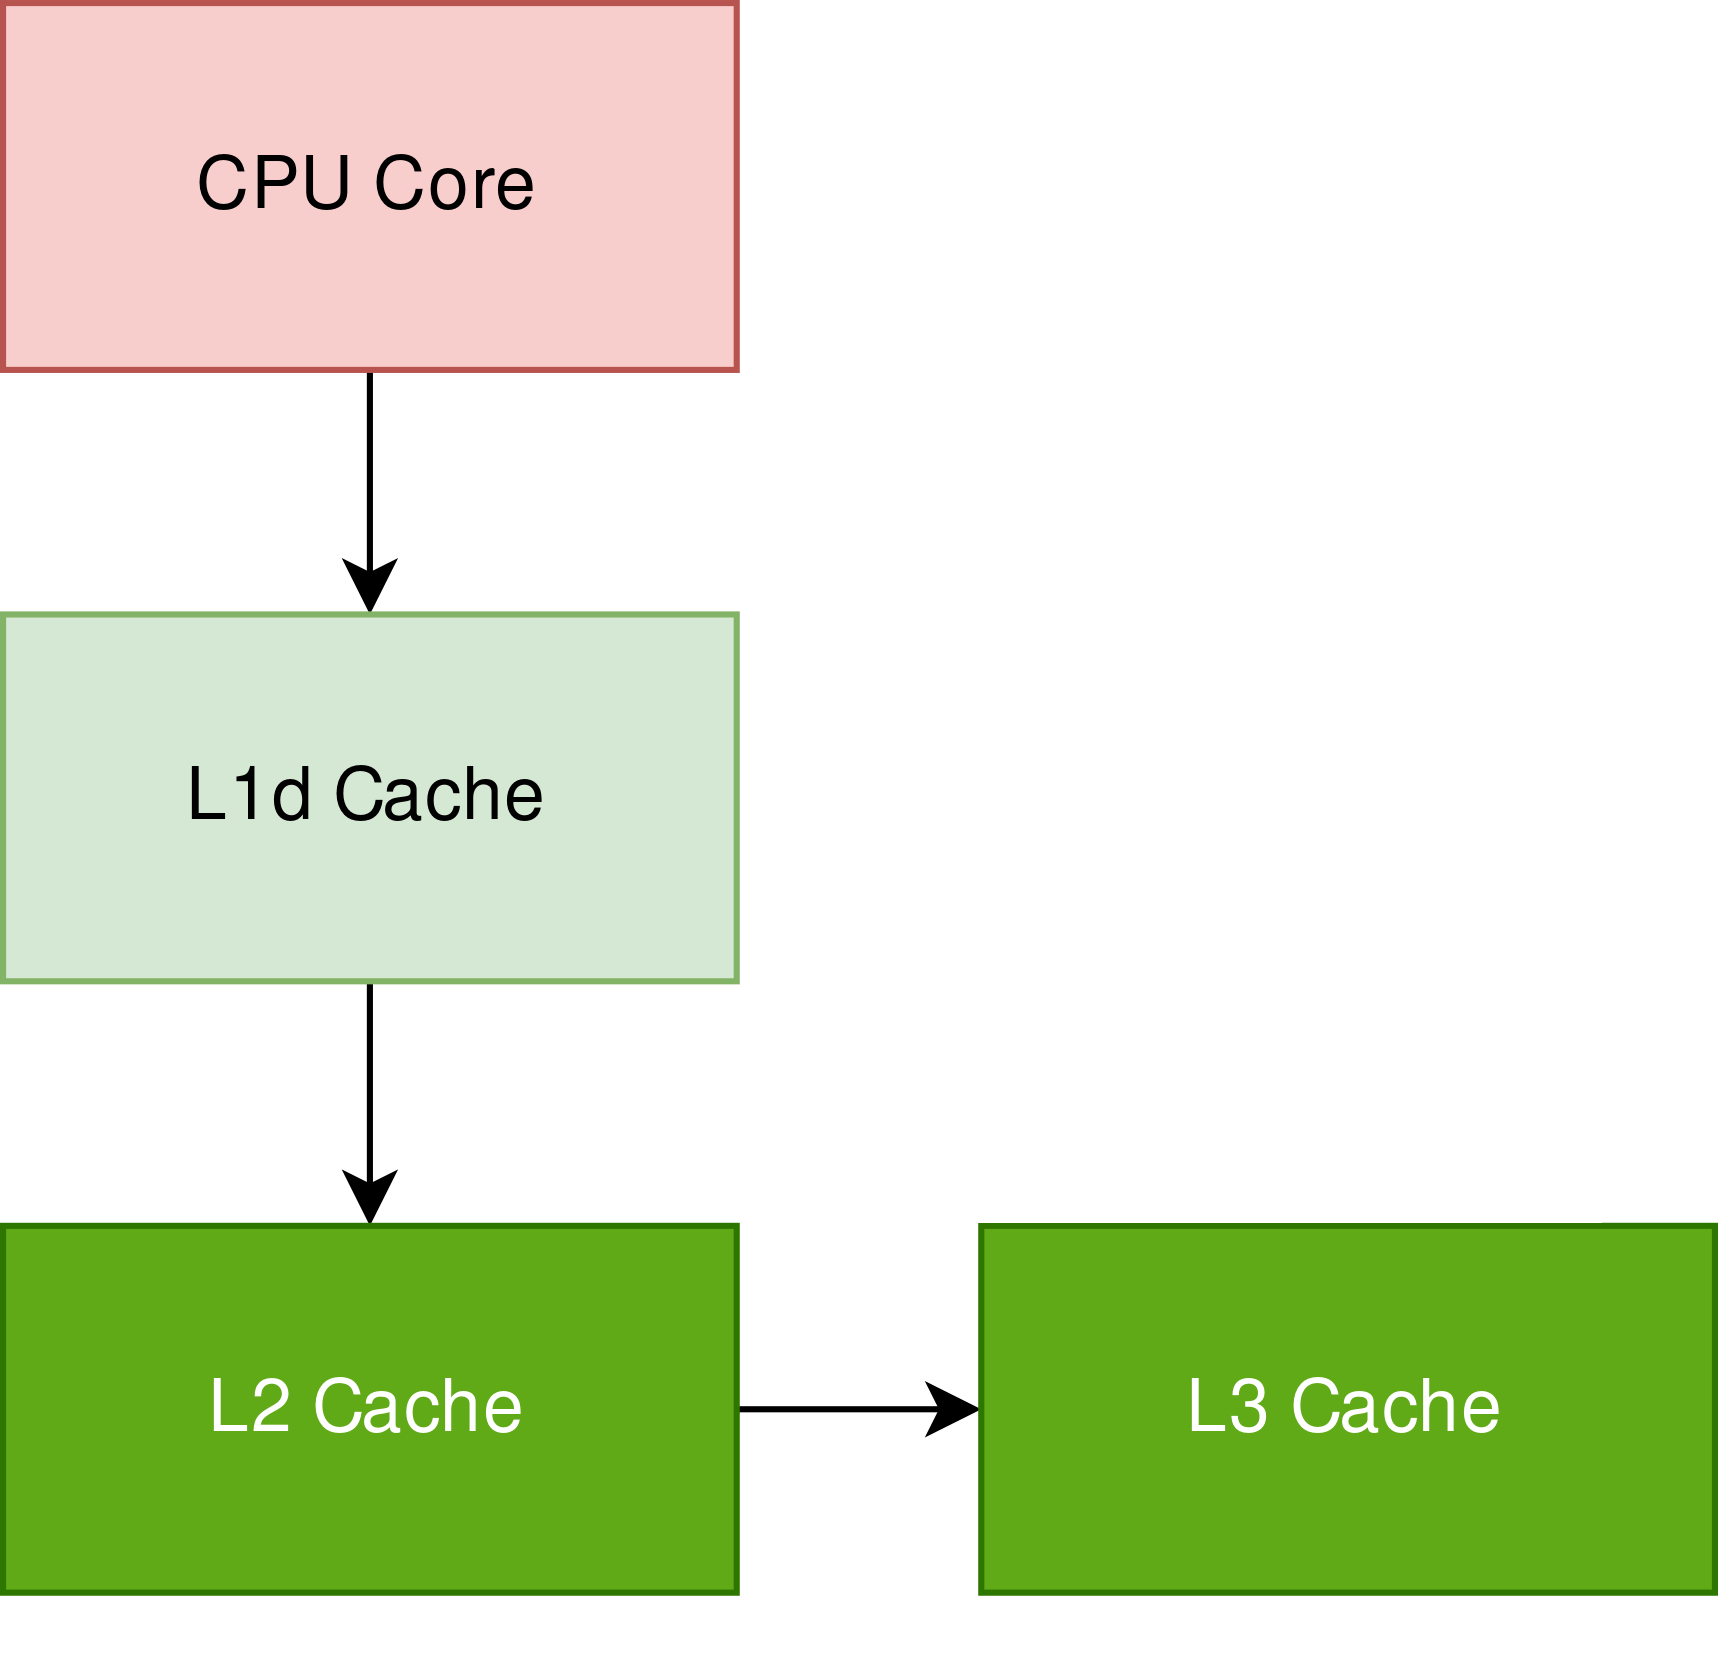
\includegraphics[height=8cm]{trace4.png}}
\end{frame}

\begin{frame}{Was passiert, wenn man auf eine Variable zugreift?}
\vspace*{0.5cm}
\centerline{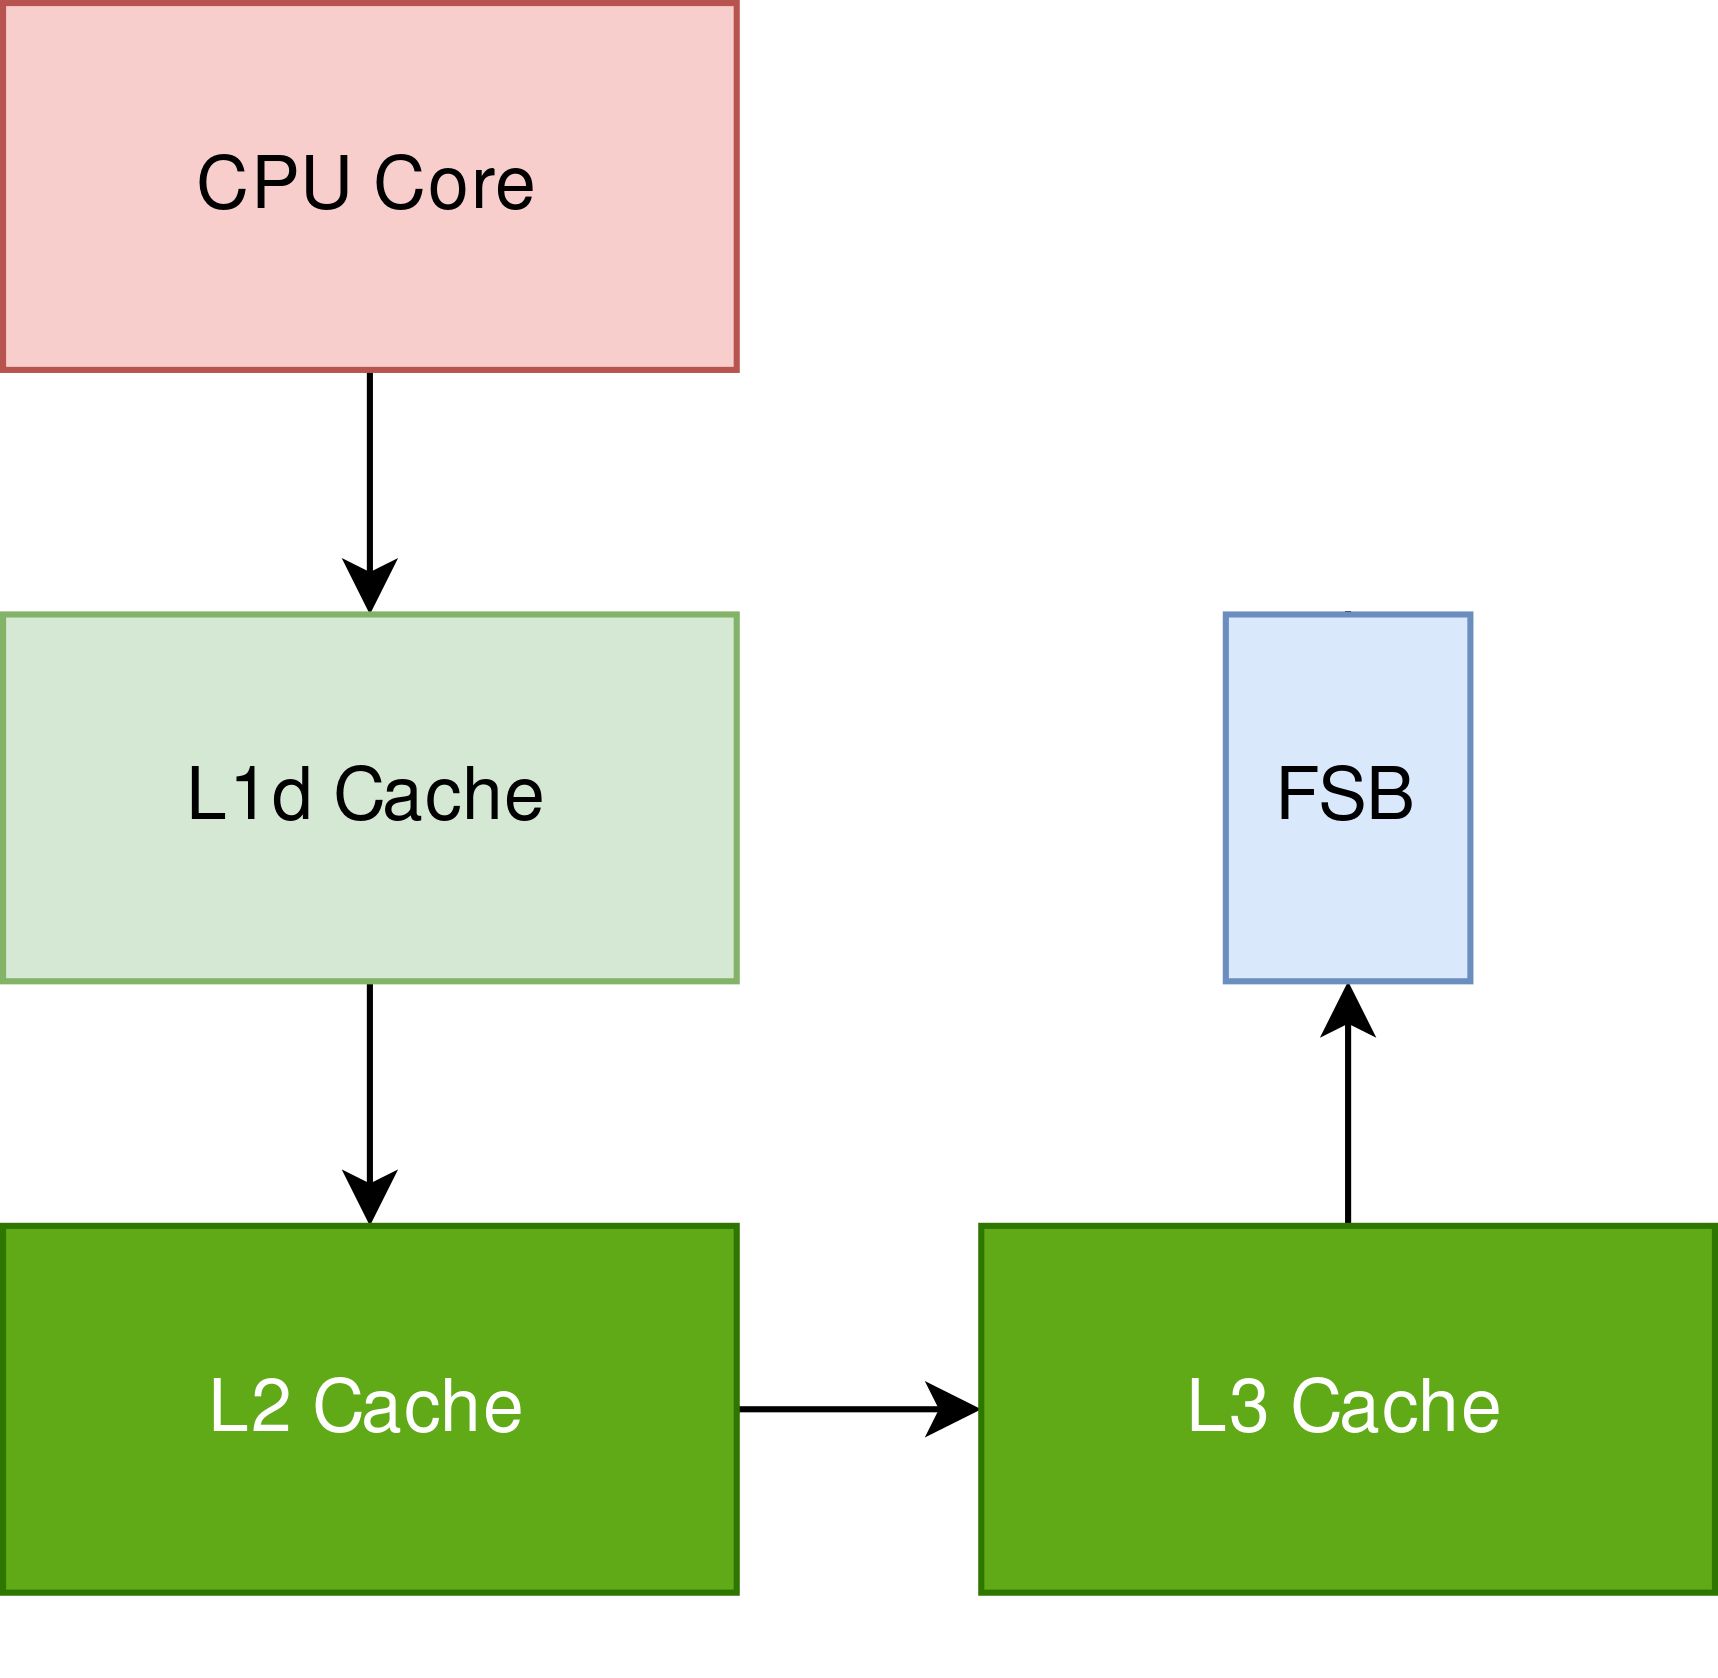
\includegraphics[height=8cm]{trace5.png}}
\end{frame}

% Dann geht alles wieder zurueck an den CPU Core, und die Daten werden in den Caches gespeichert
%
% Am Ende: 
\begin{frame}{Was passiert, wenn man auf eine Variable zugreift?}
\vspace*{0.5cm}
\centerline{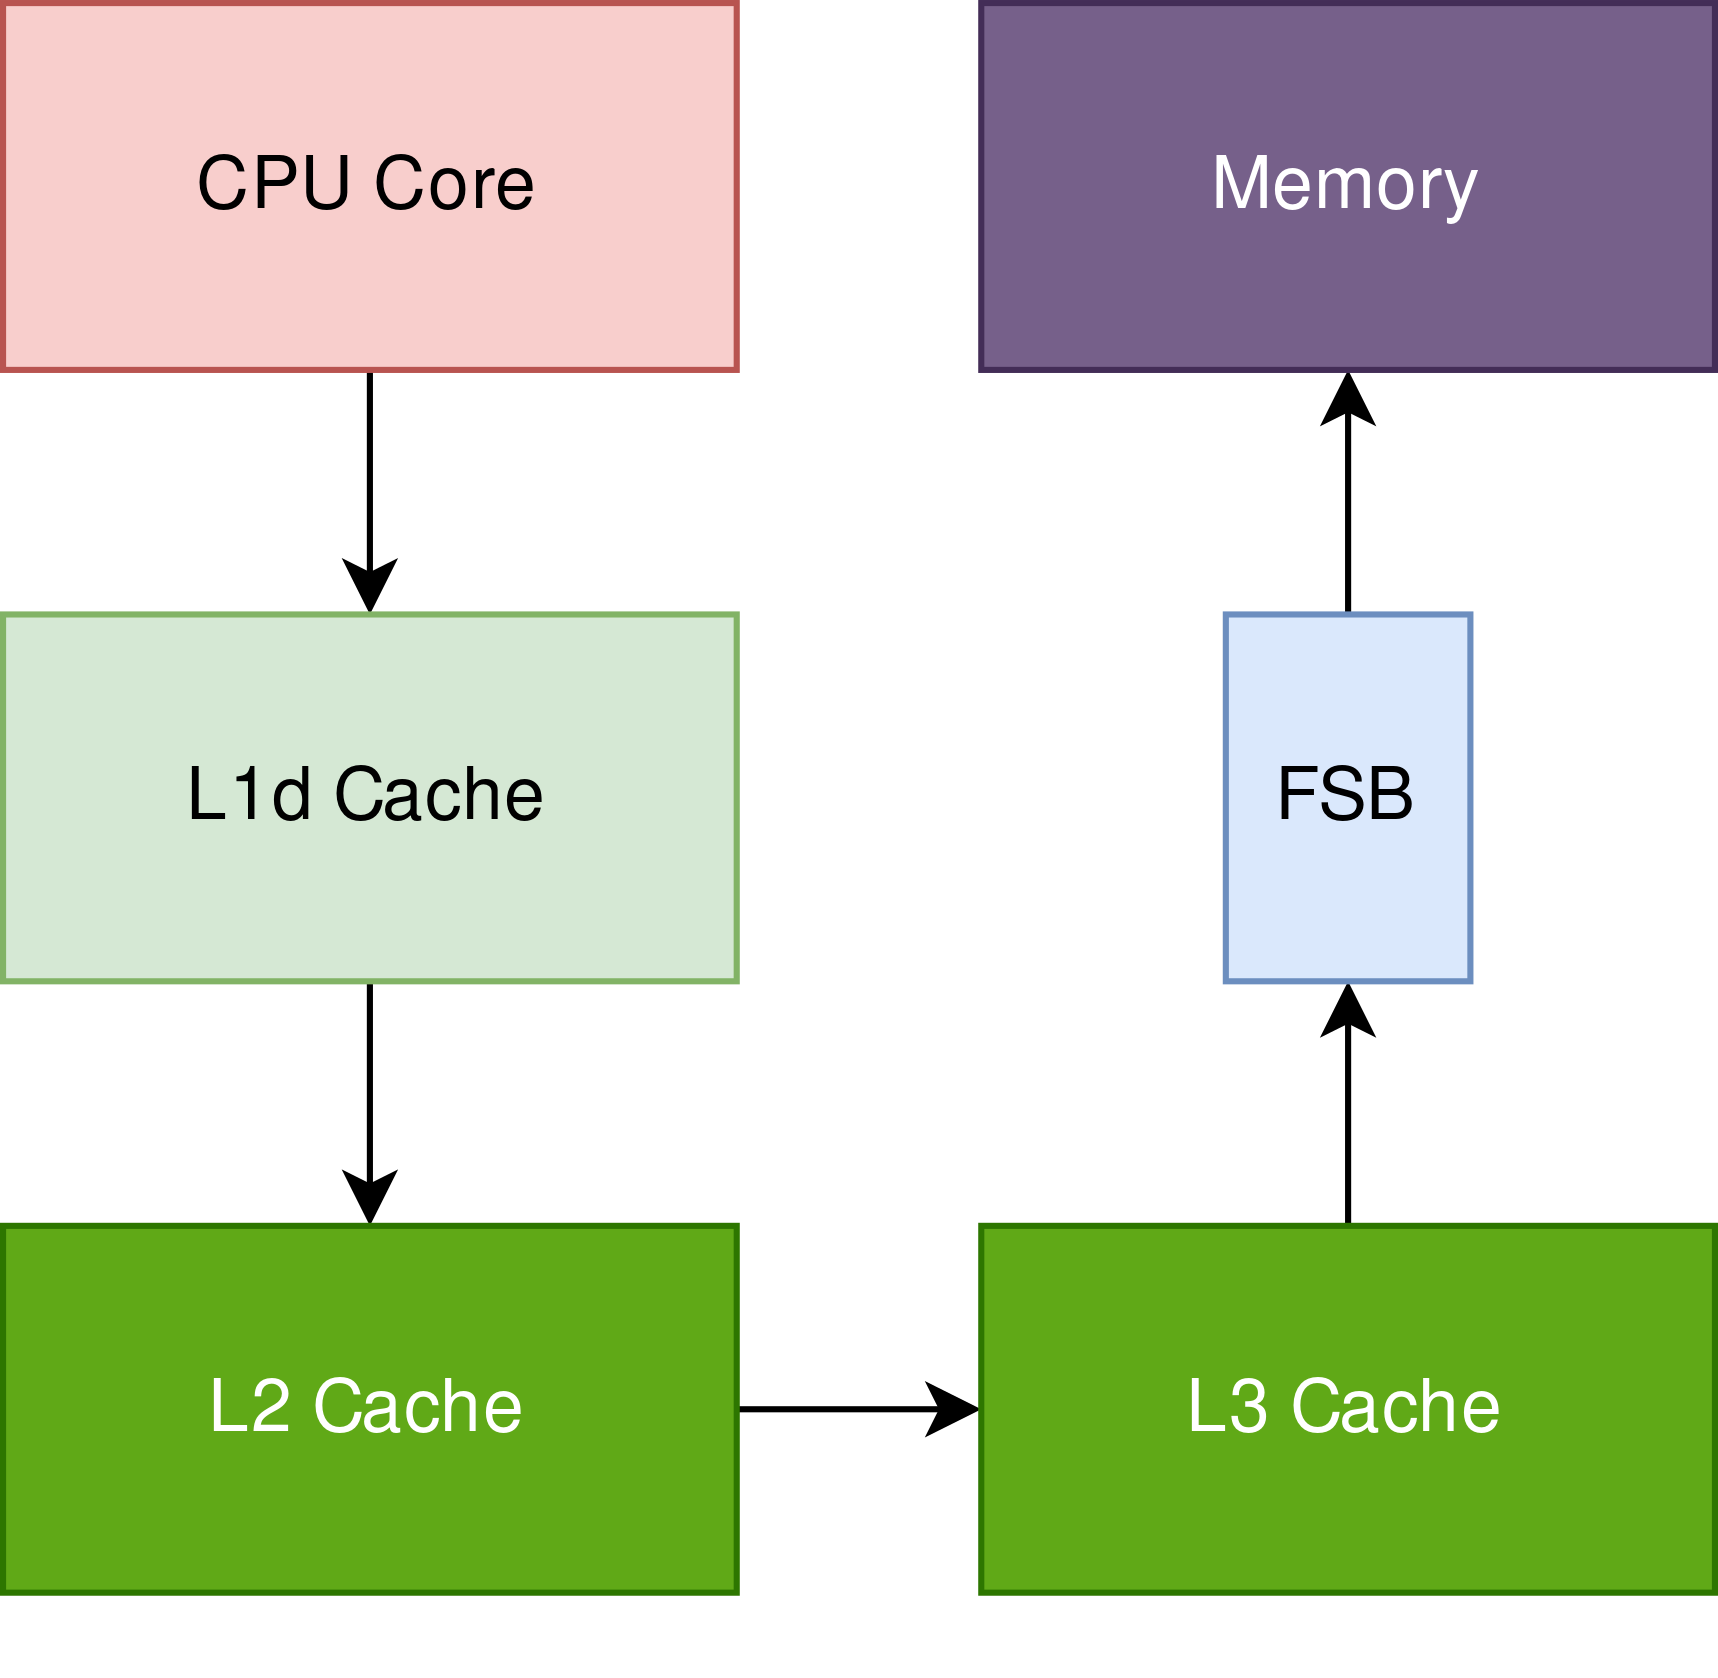
\includegraphics[height=8cm]{trace6.png}}
\end{frame}

\begin{frame}
\centering
\Huge
    Wie schnell sind die Caches?
\end{frame}


% Um ehrlich zu ein, ich war zu faul das selbst zu benchen, weil man die Caches nicht direkt
% ansprechen muss und dann so... Magie machen muss um sie zu isolieren
% <PAUSE>
% ...
% <LAST PAUSE>
% Zahlen sind doof. Lasst uns das visualisieren.
\begin{frame}
\frametitle{Wie schnell sind die Caches}
\begin{itemize}
    \item Level 1 CPU Cache: 1ns
    \\~\\\pause
    \item Level 2 CPU Cache: 4.7ns
    \\~\\\pause
    \item RAM: 83ns
    \\~\\\pause
    \item HDD: 13.7ms
\end{itemize}
\end{frame}

\begin{frame}
\frametitle{Wie schnell sind die Caches (visualisiert)}
\centerline{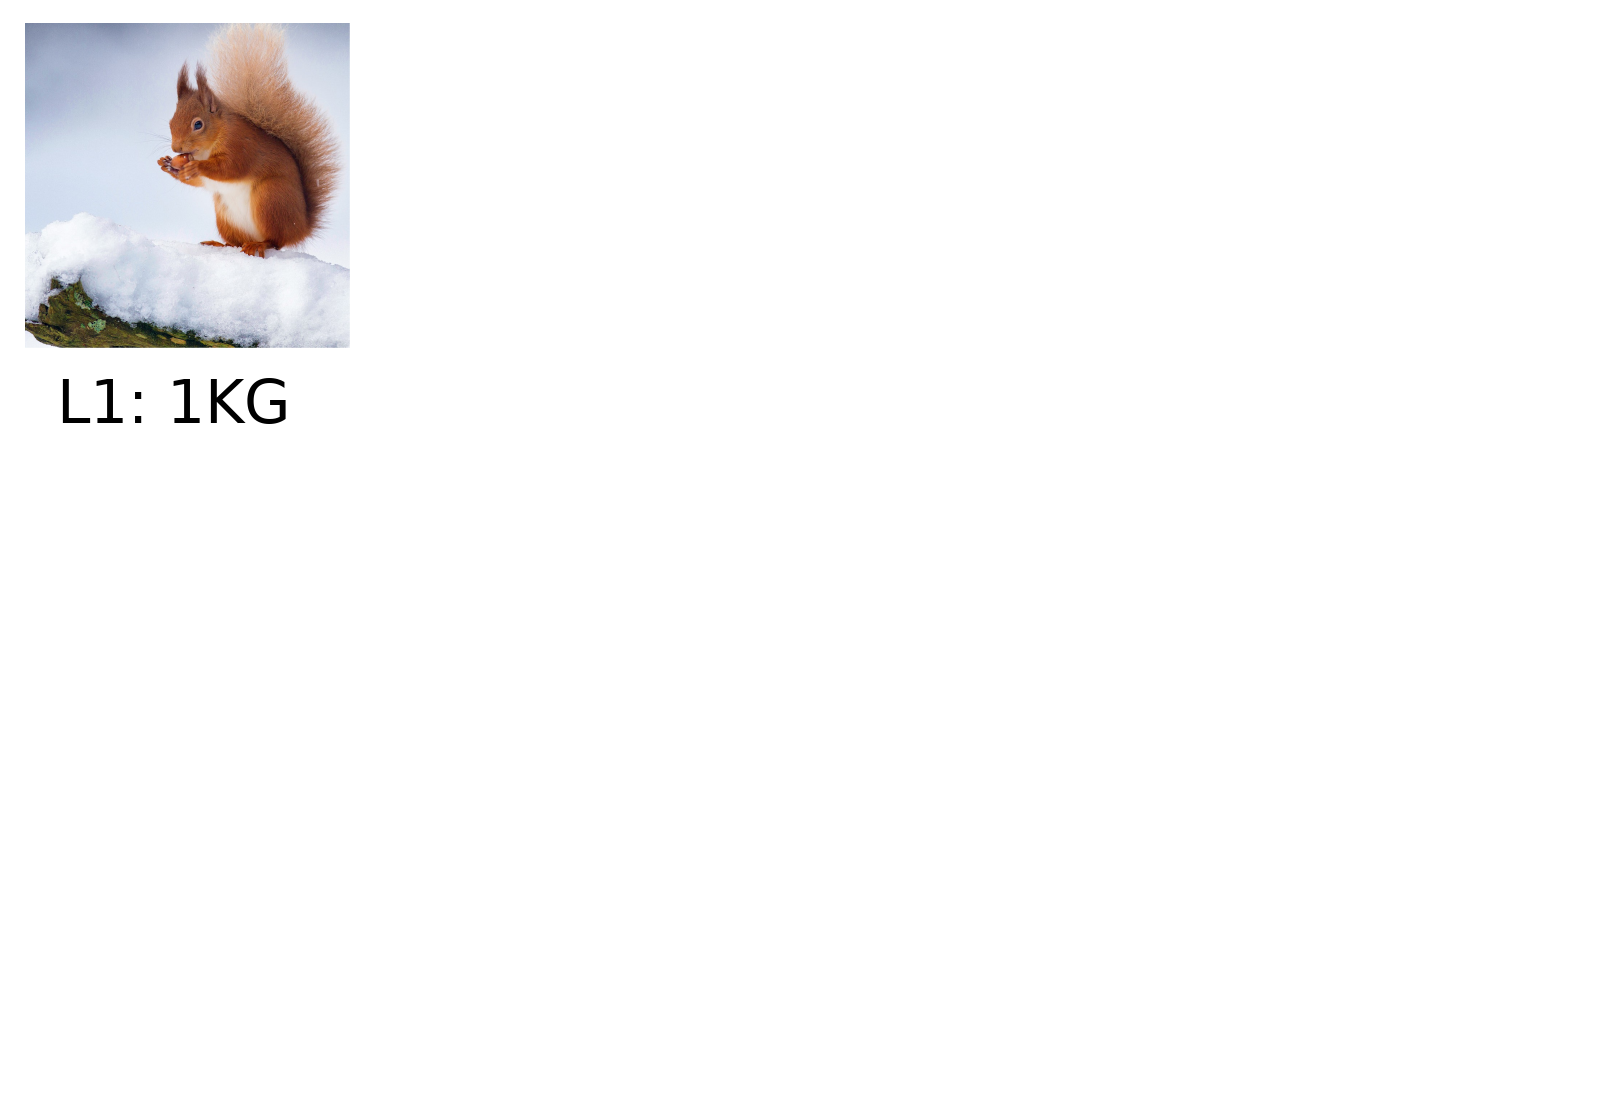
\includegraphics[width=12cm]{sizes1.png}}
\end{frame}

\begin{frame}
\frametitle{Wie schnell sind die Caches (visualisiert)}
\centerline{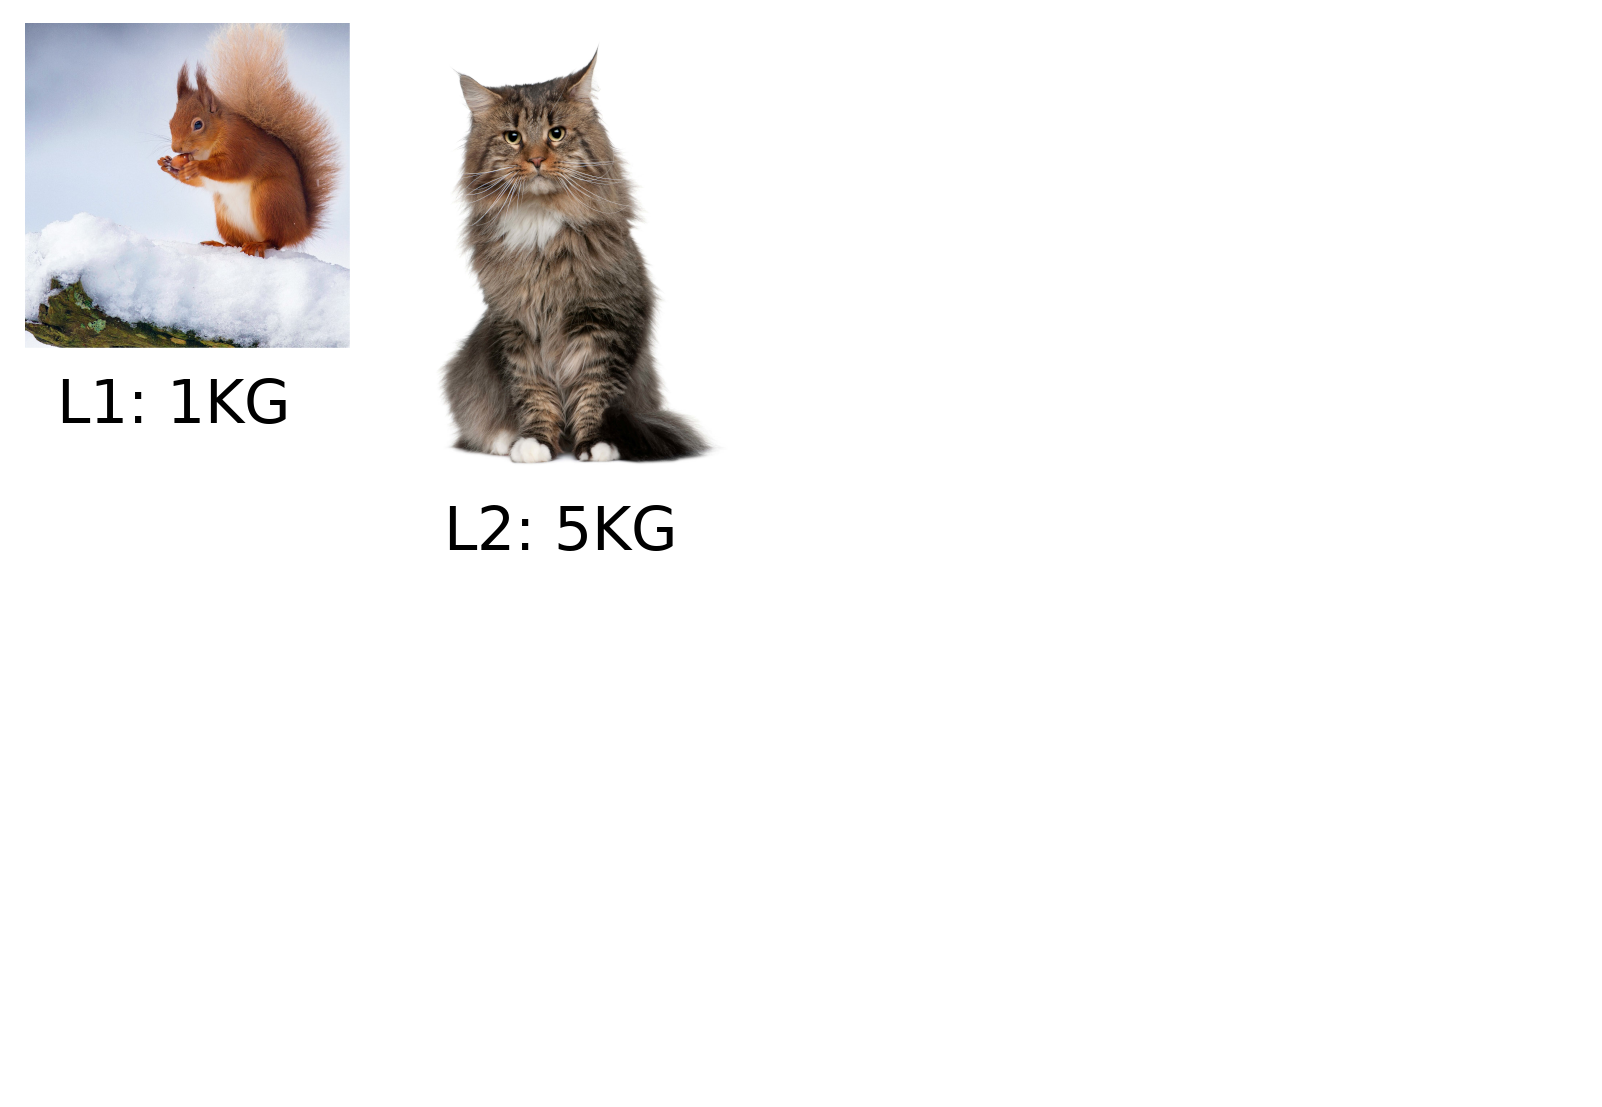
\includegraphics[width=12cm]{sizes2.png}}
\end{frame}

\begin{frame}
\frametitle{Wie schnell sind die Caches (visualisiert)}
\centerline{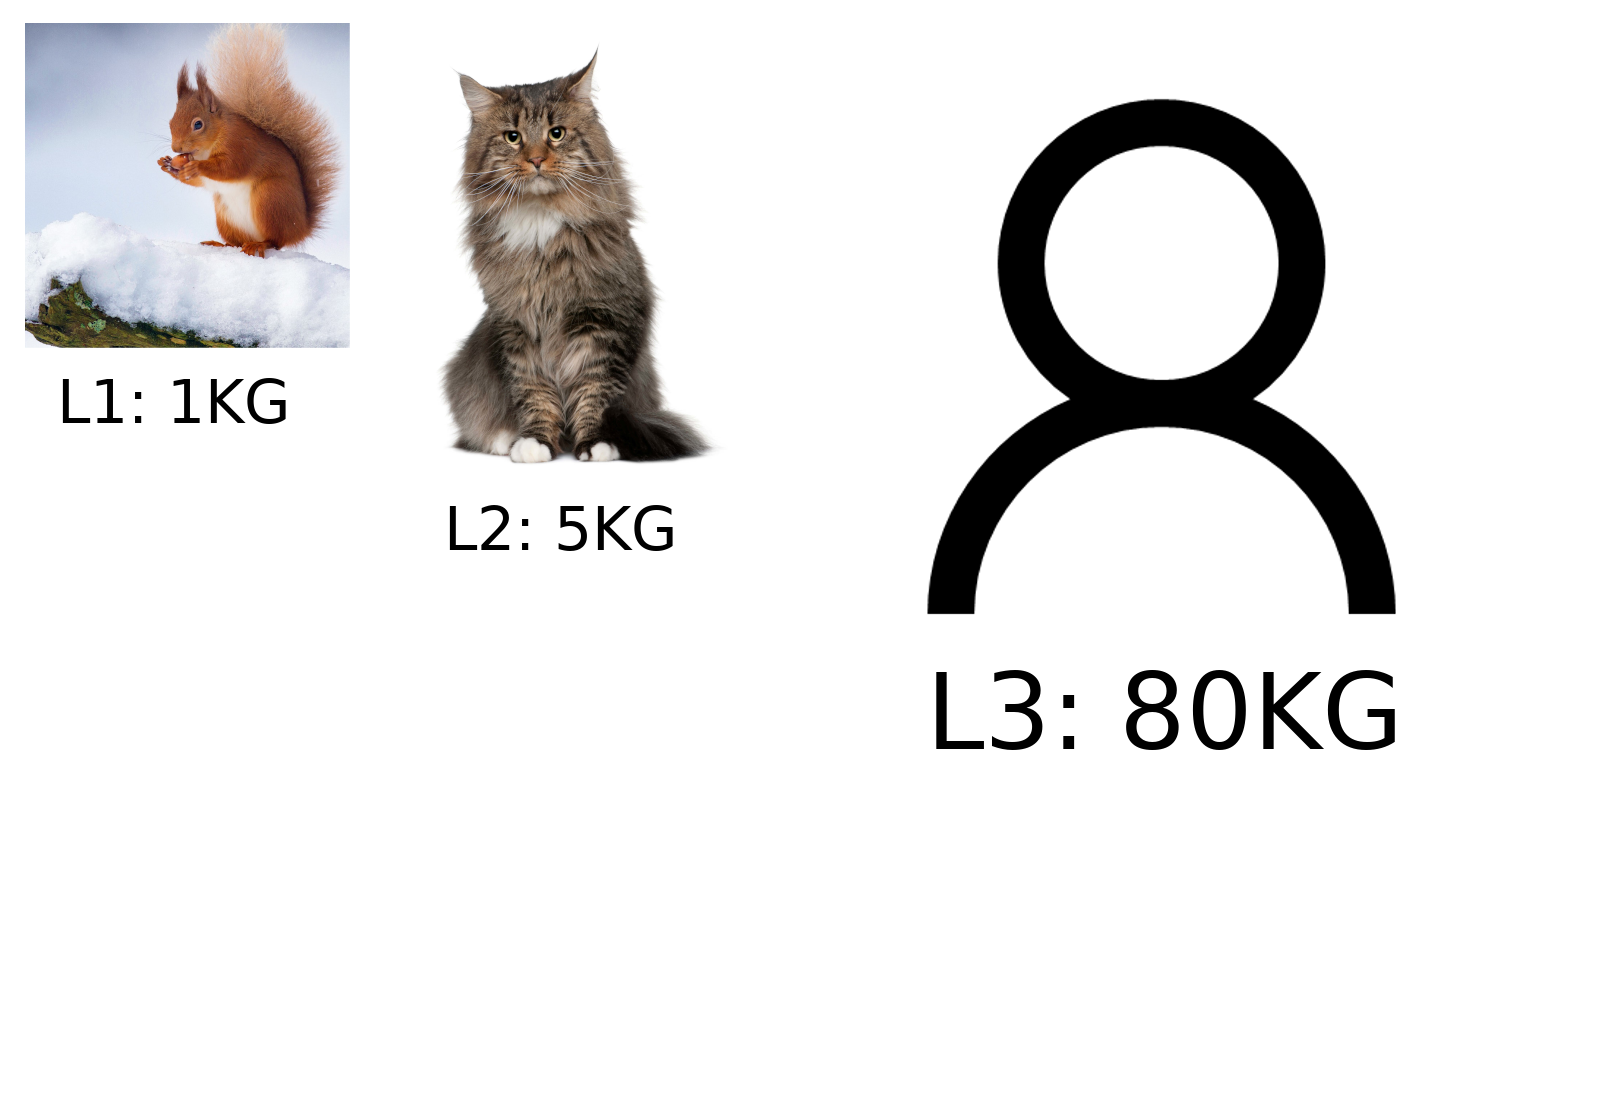
\includegraphics[width=12cm]{sizes3.png}}
\end{frame}

\begin{frame}
\frametitle{Wie schnell sind die Caches (visualisiert)}
\centerline{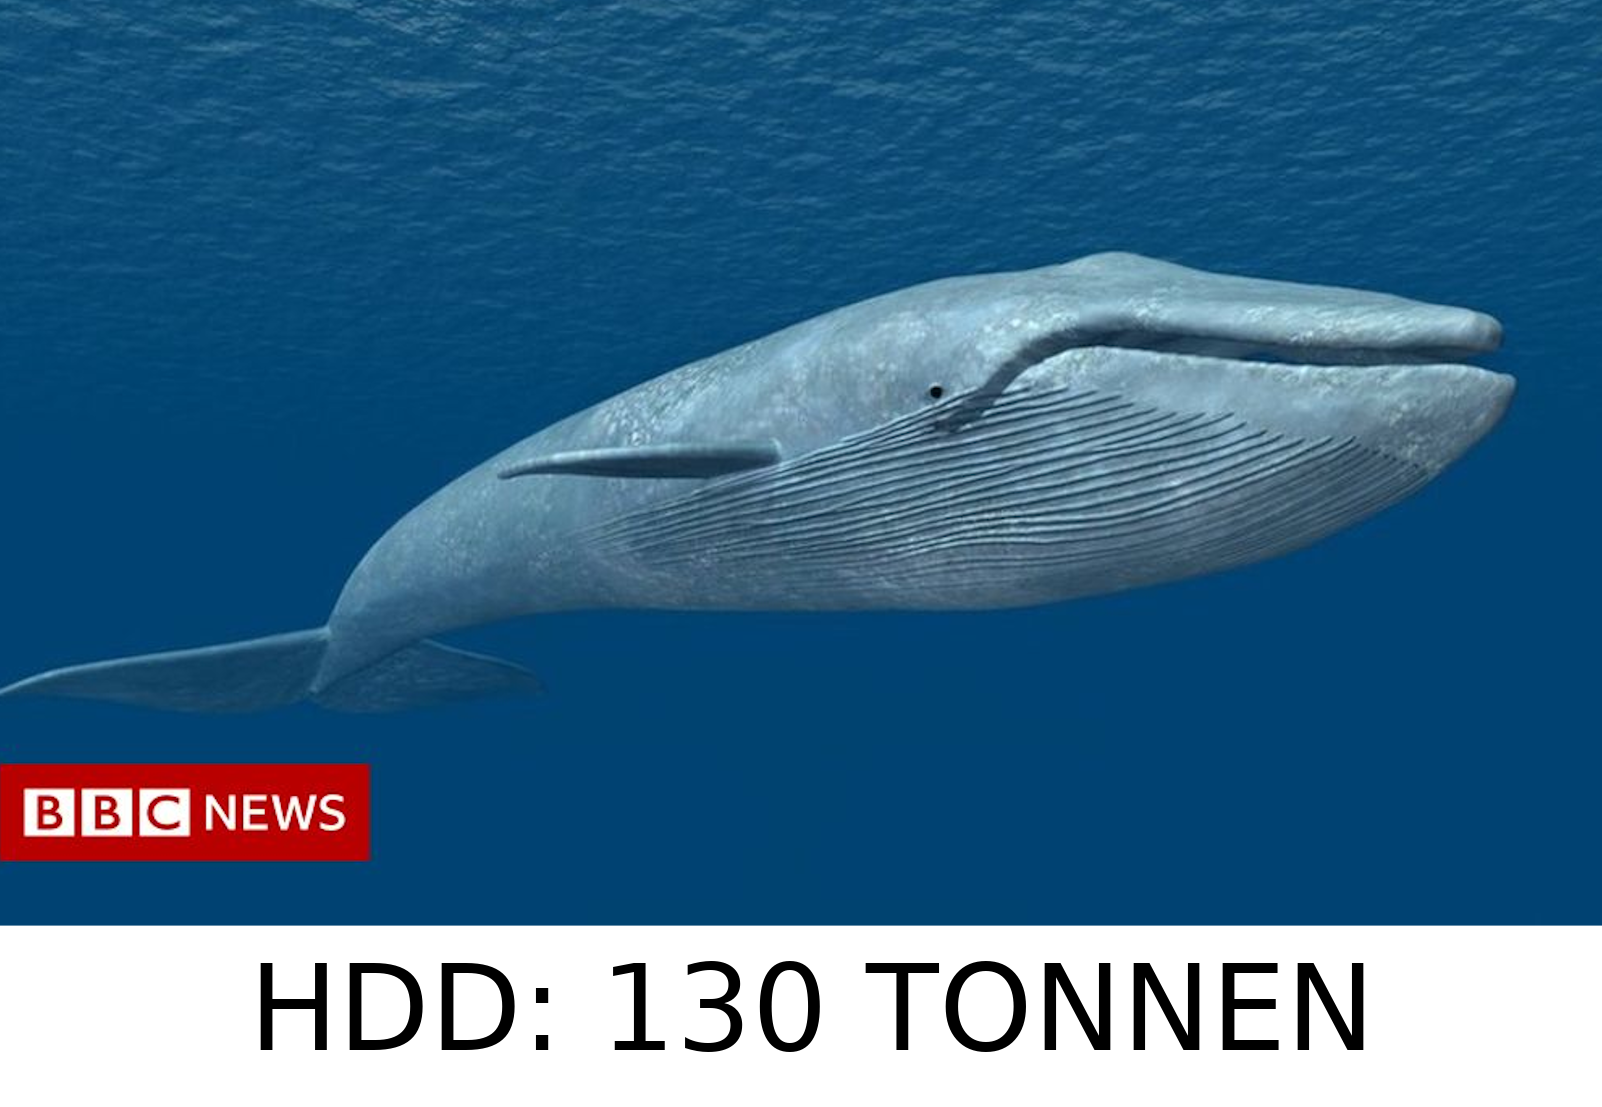
\includegraphics[width=12cm]{sizes4.png}}
\end{frame}

% Am Ende:
% - So wo wir gesehen haben wie nuetzlich es ist alles zu cachen
% - Wie funktionieren die CPU caches?
% Vorher noch ein Disclaimer
{
\usebackgroundtemplate{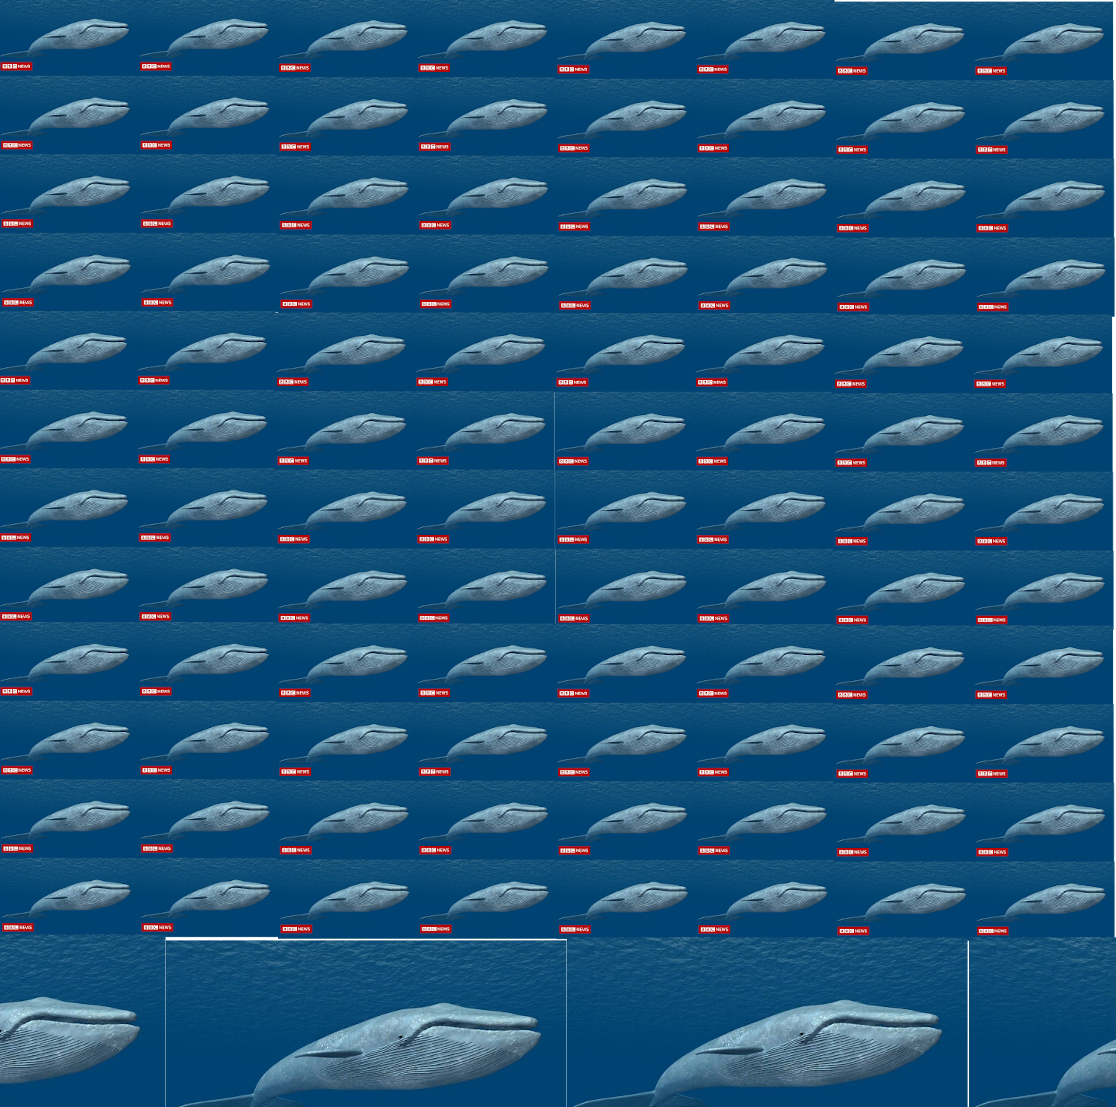
\includegraphics[width=\paperwidth, height=280px]{100_whales.png}}%
\begin{frame}
\end{frame}
}


% Am Ende: So, jetzt koennen wir uns angucken wie ein CPU Cache 
\begin{frame}
\frametitle{Wir reden im folgenden von CPU Caches}
{
\centering
CPU Caches cachen den RAM, NICHT die Festplatte\\~\\
}
\pause
Fuer Infos zu Festplattencaching: \texttt{https://linuxatemyram.com}\\~\\
\centerline{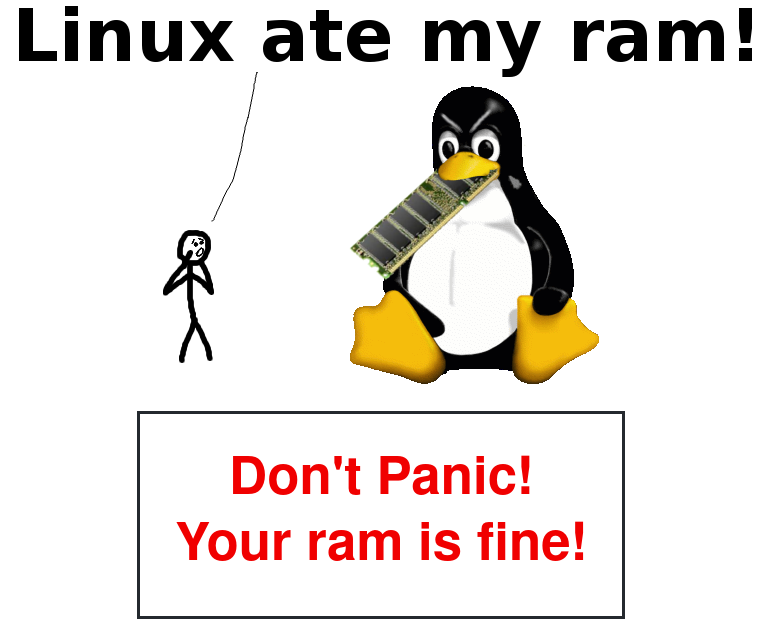
\includegraphics[height=5cm]{linuxatemyram.png}}
\end{frame}

% Am Ende:
% - Aber genau genommen sieht es eher so aus:
\begin{frame}
\frametitle{Wie ist ein CPU Cache aufgebaut? (Hier L1)}
\begin{itemize}
    \item Jeder Cache hat eine Groesse\\~\\
\end{itemize}
\centerline{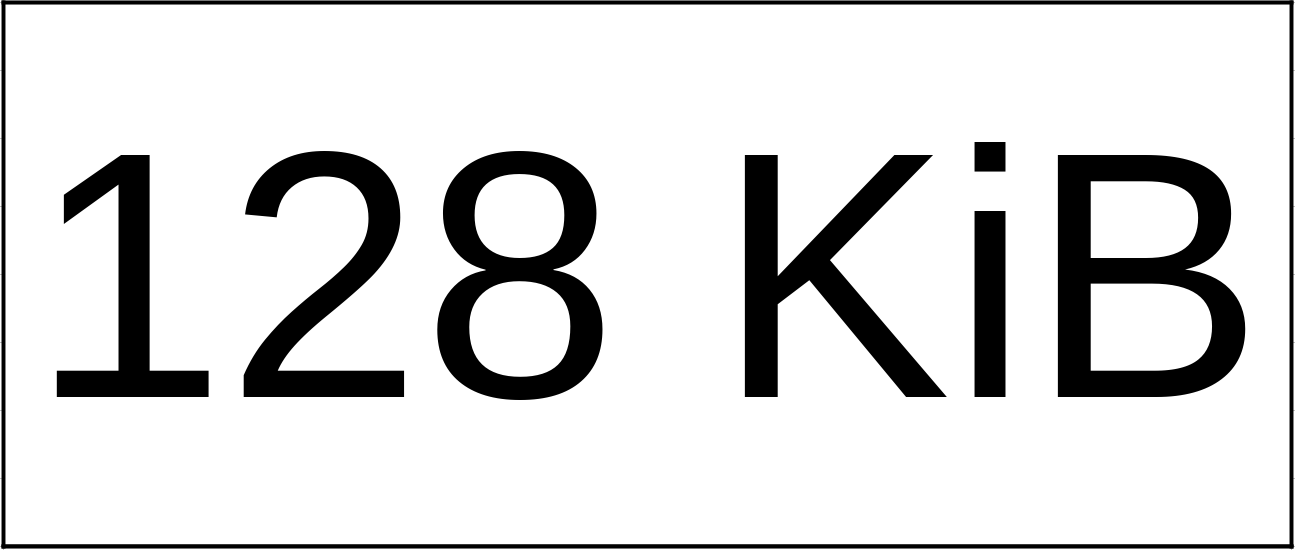
\includegraphics[width=12cm]{cell1.png}}
\end{frame}

% - Der L1 Cache wird in lines von 64 byte aufgeteilt
% - Warum macht man das? Es ist ein Tradeoff.
%   - Mehr waere effizienter (da jeder Cache-Eintrag auch Metadaten hat, somit prozentual weniger)
%   - Jeoch auch mehr verschwendet (weil man immer ganze Cache lines holen muss)
%   - Mehr misses weil man weniger cache lines hat
\begin{frame}
\frametitle{Wie ist ein CPU Cache aufgebaut? (Hier L1)}
\begin{itemize}
    \item Der Cache wird in Cache Lines aufgeteilt\\(eigentlich 2048, hier 8)\\
\end{itemize}
\centerline{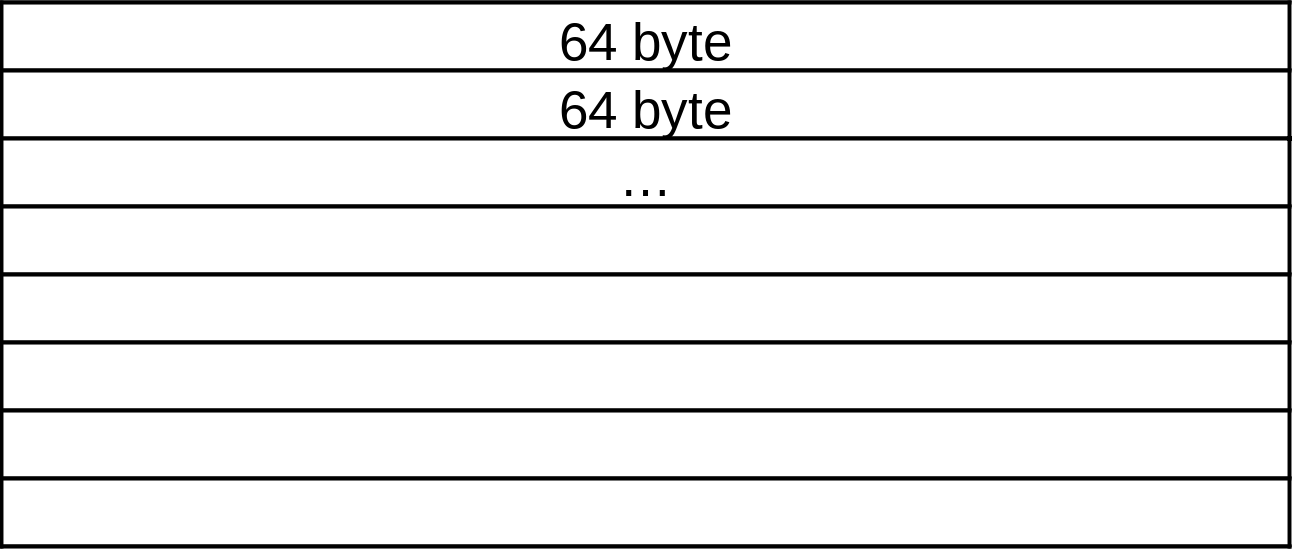
\includegraphics[width=12cm]{cell2.png}}
\end{frame}

\begin{frame}
{
\centering
\huge
Wie f\"ugen wir in den Cache ein?
}
\end{frame}

% - Erklaeren was Fully Associative Cache ist
%   - Wir speichern einfach an beliebige Stelle
% - Die roten sind alle belegt, die Gruenen sind alle frei.
% - Wir haben die folgende Addresse
%   - Das 0x heisst uebrigens nur, dass es im hexadezimalen Zahlensystem ist.
%
% - Wenn alle voll sind, dann schmeissen wir den aeltesten raus (Least recently used, LRU)
%
% - Somit nehmen wir einfach einen beliebigen freien
\begin{frame}
\frametitle{M\"oglichkeit 1: Fully Associative Cache}
\centerline{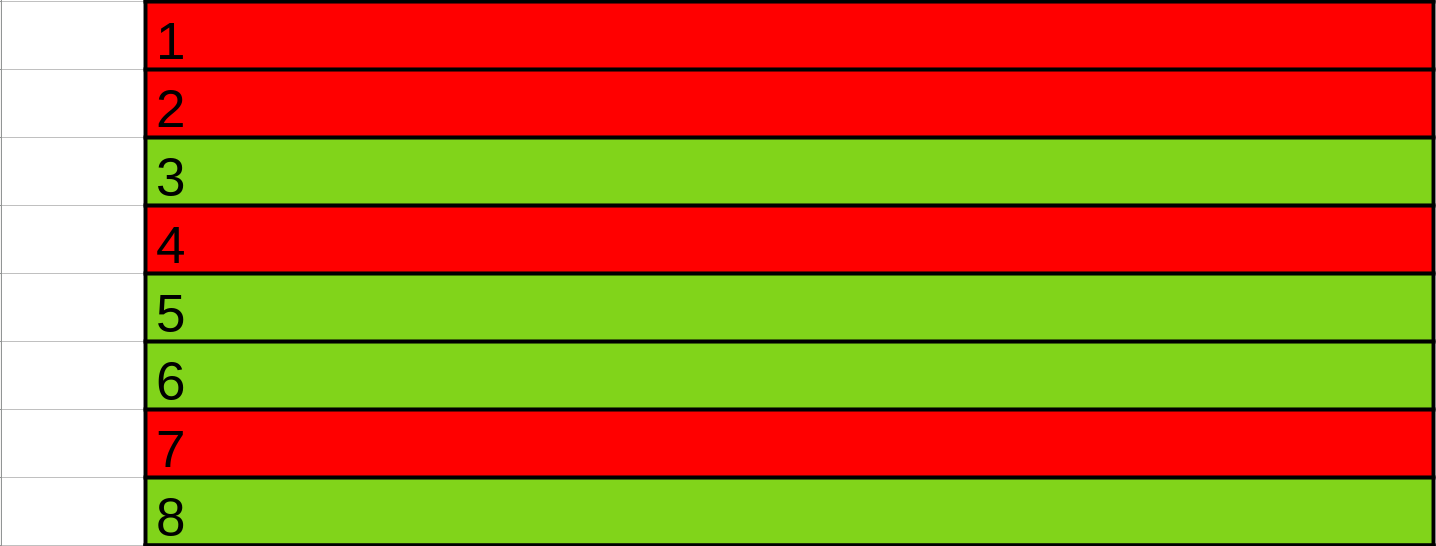
\includegraphics[width=12cm]{fac1.png}}
Adresse: 0x7ffc4322c7f4
\end{frame}


% Nun die Frage: Angenommen es kommt eine Addresse, wie finden wir heraus ob wir es im Cache haben?
\begin{frame}
\frametitle{M\"oglichkeit 1: Fully Associative Cache}
\centerline{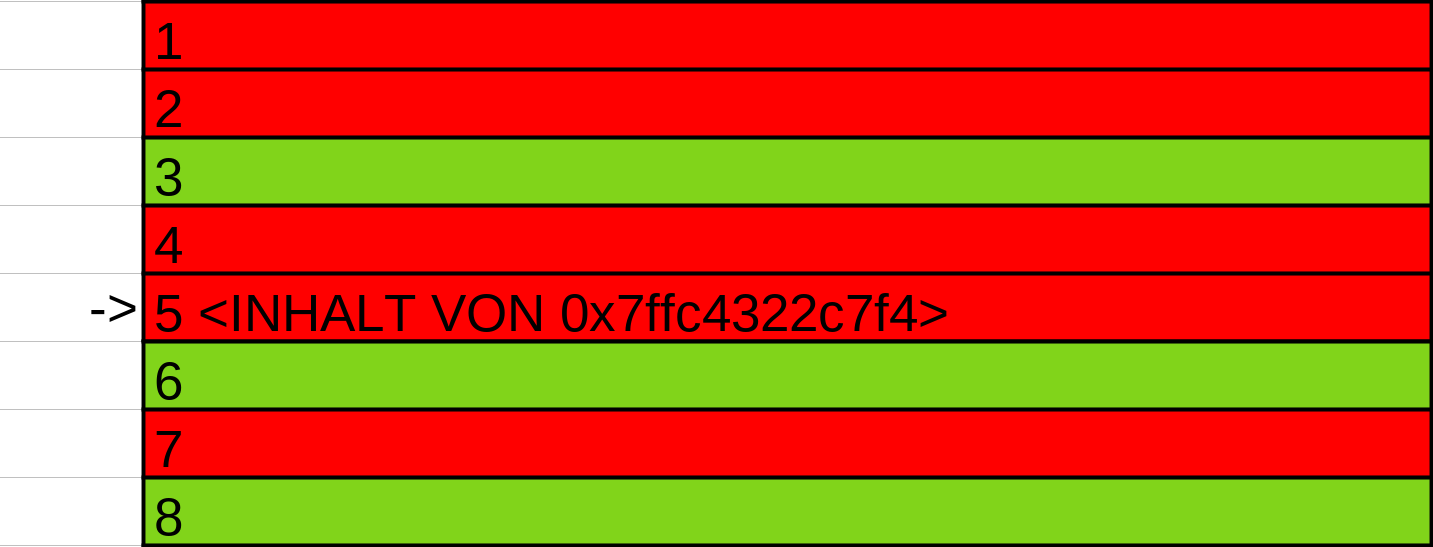
\includegraphics[width=12cm]{fac2.png}}
Adresse: 0x7ffc4322c7f4
\end{frame}

% Bei zu langsam:
%   - Bedenkt dass wir diesen drecksteuern L1 cache nur nutzen weil er so schnell ist.
%   - Wenn jeder Zugriff 4 Zyklen braucht, dann braucht das bei L1 32 Zyklen
%   - Das ist allein bei L1 Faktor 8 langsamer!
%
% Bei zu teuer:
%   - Mein L1i cache hat alleine 1024 lines 
\begin{frame}
\frametitle{Ist mein aktueller Wert im Cache?}
\begin{block}{M\"oglichkeit 1: Wir gehen \"uber alle Werte und gucken nach}
\begin{itemize}
\pause
\item Theoretisch moeglich
\pause
\item aber VIEL zu langsam!
\end{itemize}
\end{block}
\pause
\begin{block}{M\"oglichkeit 2: Wir gucken alle gleichzeitig nach}
\begin{itemize}
\pause
\item Auch theoretisch moeglich
\pause
\item aber VIEL zu teuer!
\end{itemize}
\pause
\end{block}
\begin{block}{Fazit: F\"ur aktuelle Cache-Gr\"o\ss{}en unbrauchbar!}
\end{block}
\end{frame}

% Fuer direct mapped cache entscheiden wir anhand der Addresse einen Platz.
% Lasst uns die Addresse kurz in Binaer umwandeln.
\begin{frame}
\frametitle{M\"oglichkeit 2: Direct Mapped Cache}
\centerline{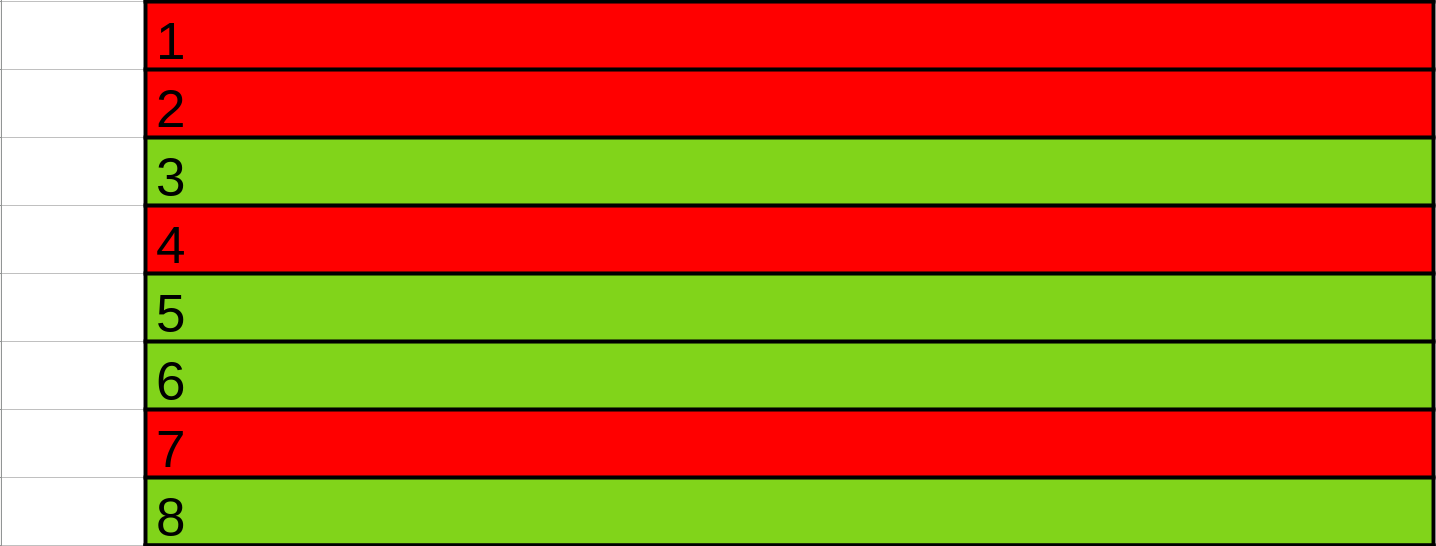
\includegraphics[width=12cm]{fac1.png}}
Adresse: 0x7ffc4322c7f4
\end{frame}

% Okay, wie entscheiden wir nun aus der Addresse welche der 8 Cache Lines wir nehmen?
%
% - Wir erinnern uns dass eine line 64 byte sind. Also beschreiben die letzten 6 bit in der
%   Adresse nur, welchen Teil wir haben wollen.
%   - Weil man mit 6 bit 2^6 Zahlen darstellen kann.
%   - Trennen wir den Teil mal ab.
\begin{frame}
\frametitle{M\"oglichkeit 2: Direct Mapped Cache}
\centerline{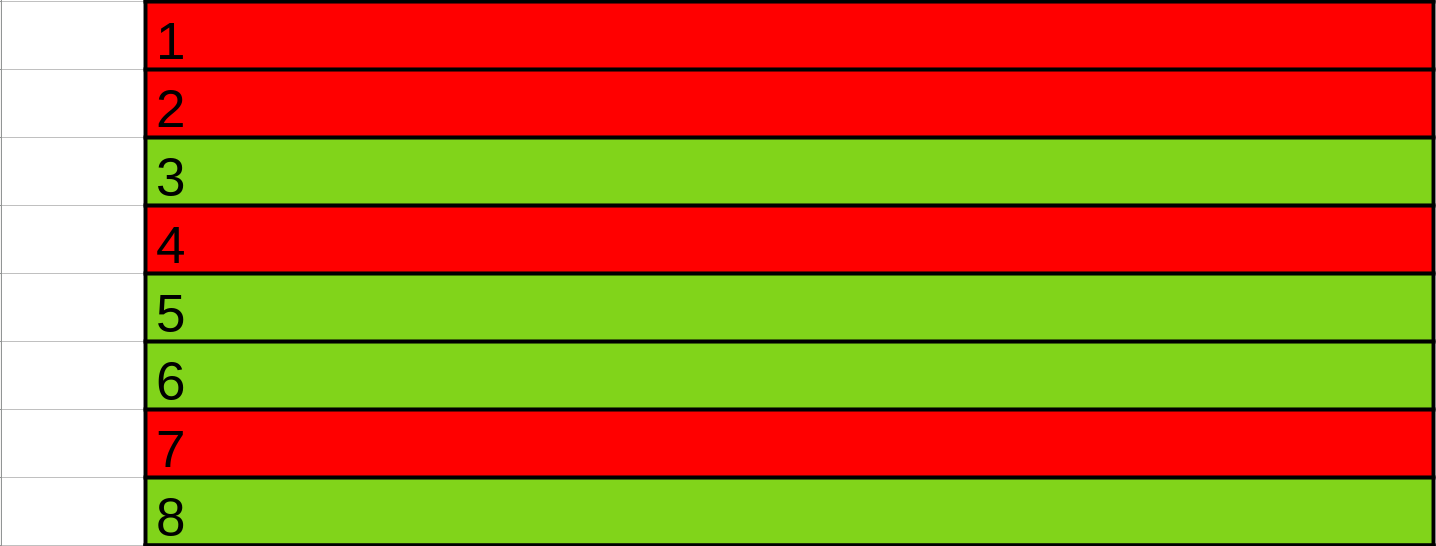
\includegraphics[width=12cm]{fac1.png}}
011111111111110001000011001000101100011111110100
\end{frame}

% Fuer 8 Speicherstellen brauchen wir 3 bits (0-1, 2-3, 4-7)
% 
% Nun ist die Frage: Nehmen wir die von Links oder rechts?
%
% Meistens liesst man Daten hintereinander. Somit haben die die selben oberen Stellen.
% Damit es sich auf verschiedene cache lines verteilt, lass uns die unteren nehmen!
\begin{frame}
\frametitle{M\"oglichkeit 2: Direct Mapped Cache}
\centerline{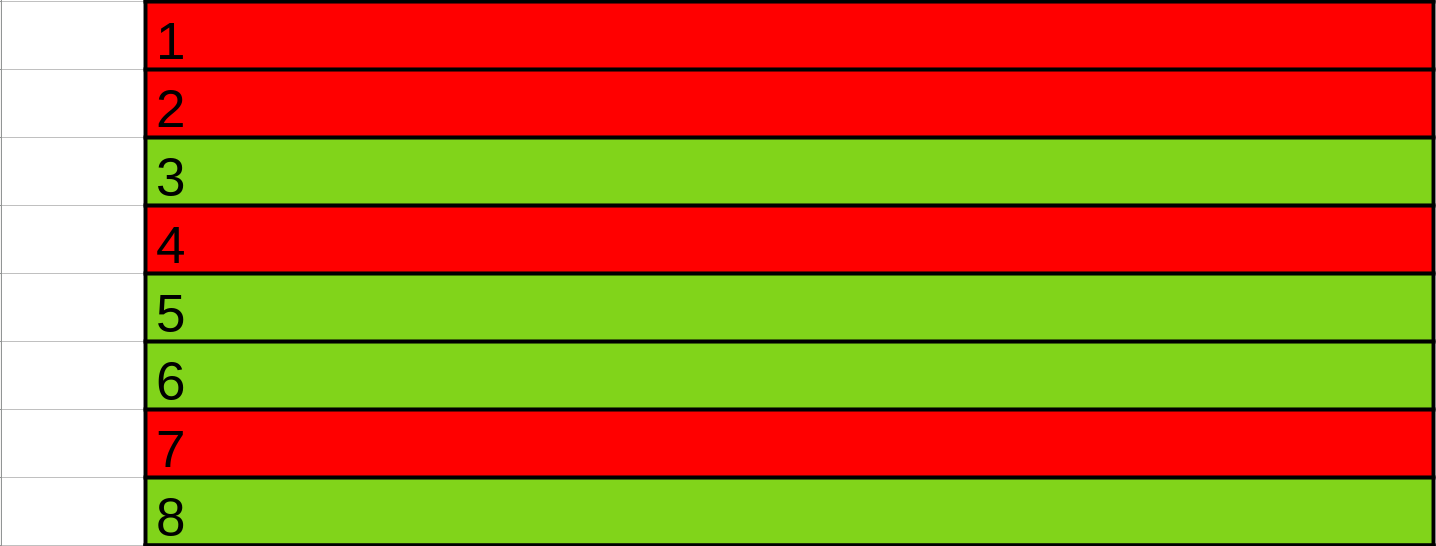
\includegraphics[width=12cm]{fac1.png}}
011111111111110001000011001000101100011111 {\color{orange}110100}
\end{frame}

% Den restlichen Teil nehmen wir dann einfach, um zu gucken ob da auch unsere Addresse drin ist.
% Weil es koennen ja Kollisionen passieren, blablabla
% Den Teil speichern wir mit in die Zelle.
\begin{frame}
\frametitle{M\"oglichkeit 2: Direct Mapped Cache}
\centerline{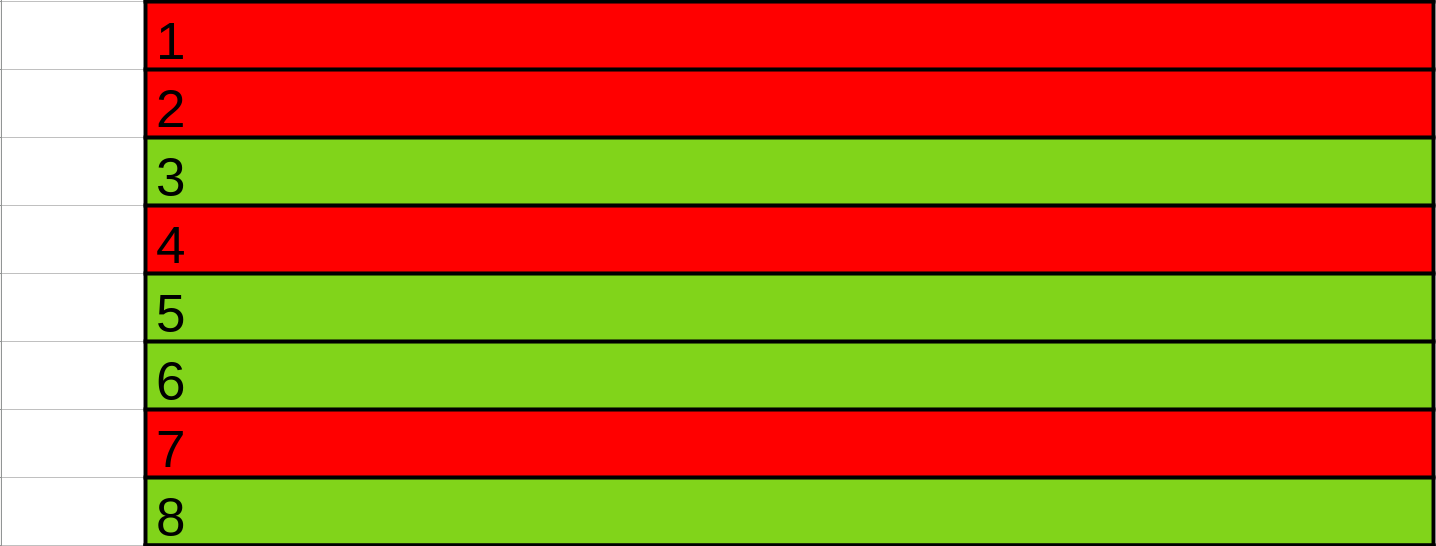
\includegraphics[width=12cm]{fac1.png}}
011111111111110001000011001000101100011 {\color{blue}111} {\color{orange}110100}
\end{frame}

% Nun lass es uns mal in Binaer umwandeln
\begin{frame}
\frametitle{M\"oglichkeit 2: Direct Mapped Cache}
\centerline{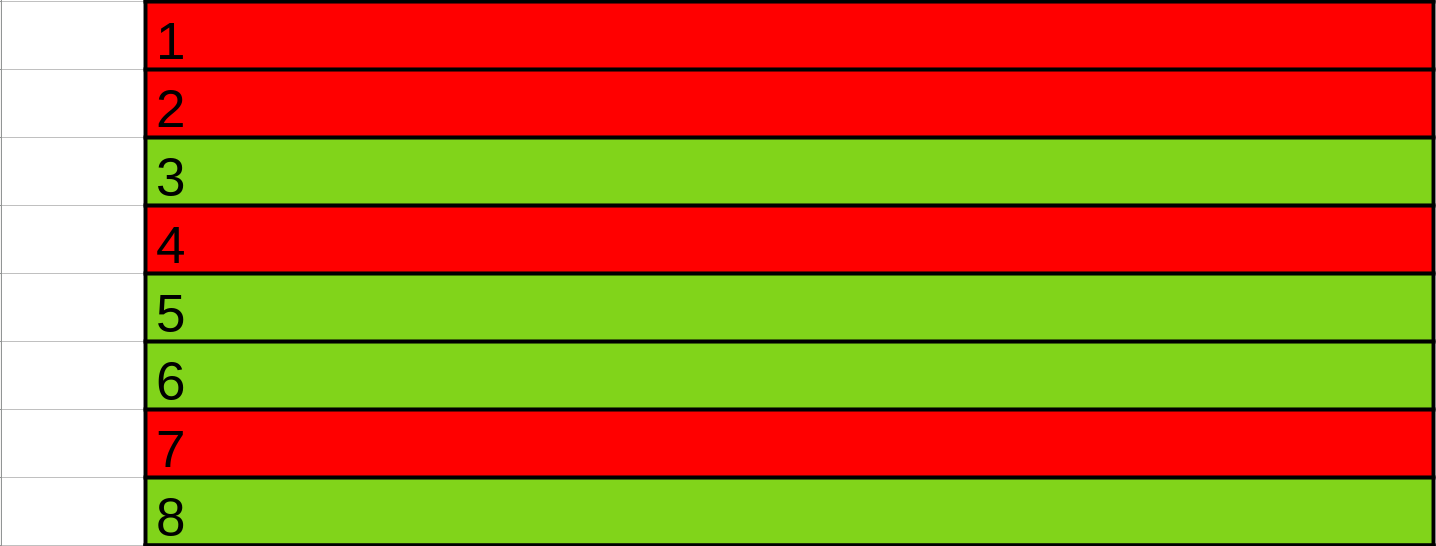
\includegraphics[width=12cm]{fac1.png}}
{\color{brown}011111111111110001000011001000101100011} {\color{blue}111} {\color{orange}110100}
\end{frame}

% Somit speichern den Inhalt der Addresse in
% - Zelle 8 (binaerzahlen sind 0 indexiert)
% - mit Pruefzahl 274.846.552.419 ab
% und wir wollen eigentlich nur
% - ab Offset 52!
\begin{frame}
\frametitle{M\"oglichkeit 2: Direct Mapped Cache}
\centerline{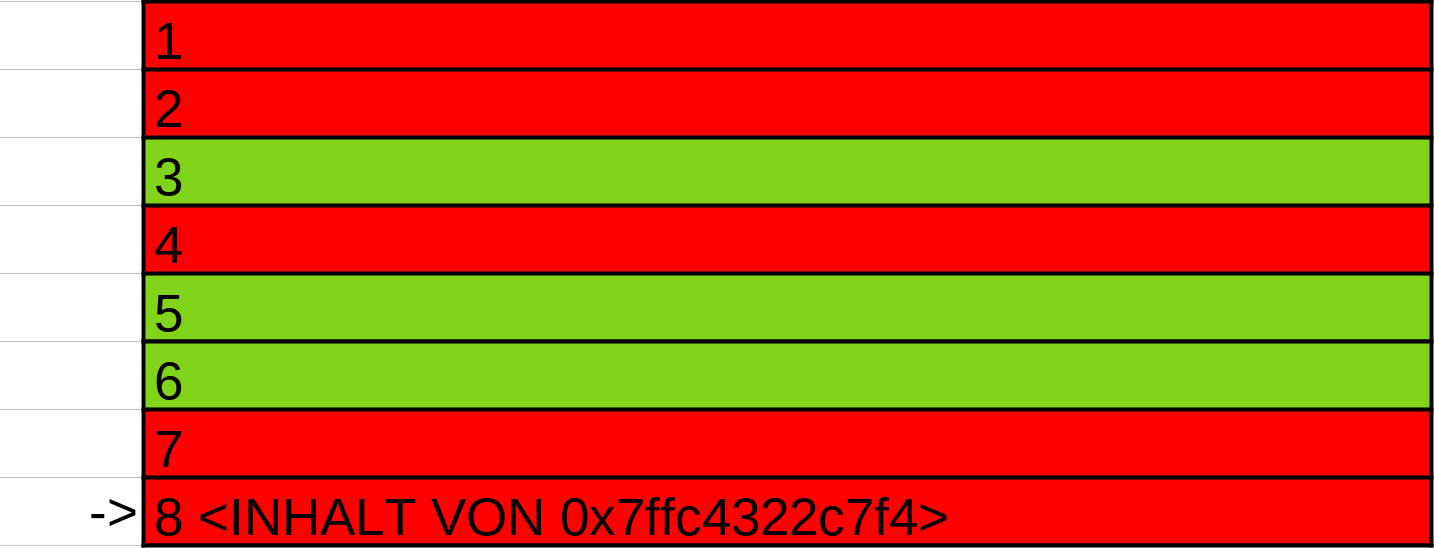
\includegraphics[width=12cm]{dmc1.png}}
{\color{brown}274.846.552.419} {\color{blue}7} {\color{orange}52}\\
\pause
Leider gibt es eine Problematik...
\end{frame}

% Nach dem ersten:
%   - Nun gehen wir im Speicher weiter und ueberschreiten die Cache Line Grenze
% Vor der Kollision:
%   - Nun lesen wir eine globale Variable ein.
%
% Am Ende:
%   - Die Loesung: Wir vermischen beides!
\begin{frame}
\frametitle{Eine Problematik}
Lasst uns ein paar Adressen durchgehen.
\pause
\begin{itemize}
    \item {\color{brown}274.846.552.419} {\color{blue}7} {\color{orange}52}
    \pause
    \item {\color{brown}274.846.552.419} {\color{blue}8} {\color{orange}0}
    \pause
    \item {\color{brown}319.257.156.827} {\color{blue}7} {\color{orange}32}
    \pause
\end{itemize}
Mit 3 Variablen hatten wir bereits eine Kollision!\\\pause
Kein effizient genutzter Speicher.
\end{frame}


% Die einzelnen Mengen werden wie ein Direct Mapped Cache angesprochen
%   - Somit koennen wir in 4 Zyklen (durch unser Pseudohashing) nachgucken wohin es muss
% Jede Menge ist intern Associatively Cached. Sprich der Platz ist beliebig.
%   - Somit muessen wir nur $n$ nachgucken, bei mir im PC ist n=8.
%   - Das ist noch gut bezahlbar, 8 gleichzeitig nachzugucken.
%
% Das ist so ein bisschen wie offenes Hashing, wo man am Ende der Buckets ne LinkedList hat.
%
% Also wandeln wir es wieder in binaer um:
\begin{frame}
\frametitle{M\"oglichkeit 3: $n$-way Associative Cache (hier $n=2$)}
\centerline{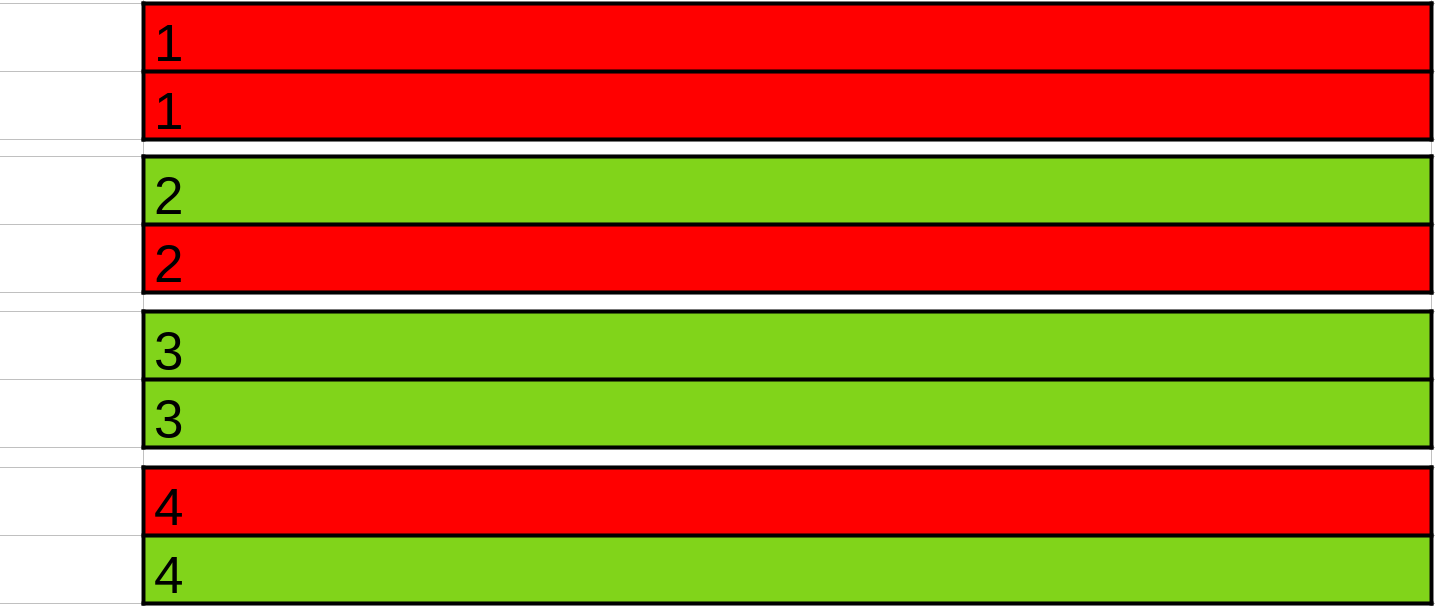
\includegraphics[width=12cm]{nac1.png}}
Adresse: 0x7ffc4322c7f4
\end{frame}

% Die Cache line sizes sind immer noch 64 byte.
% Also koennen wir die Offset wieder ignorieren.
\begin{frame}
\frametitle{M\"oglichkeit 3: $n$-way Associative Cache (hier $n=2$)}
\centerline{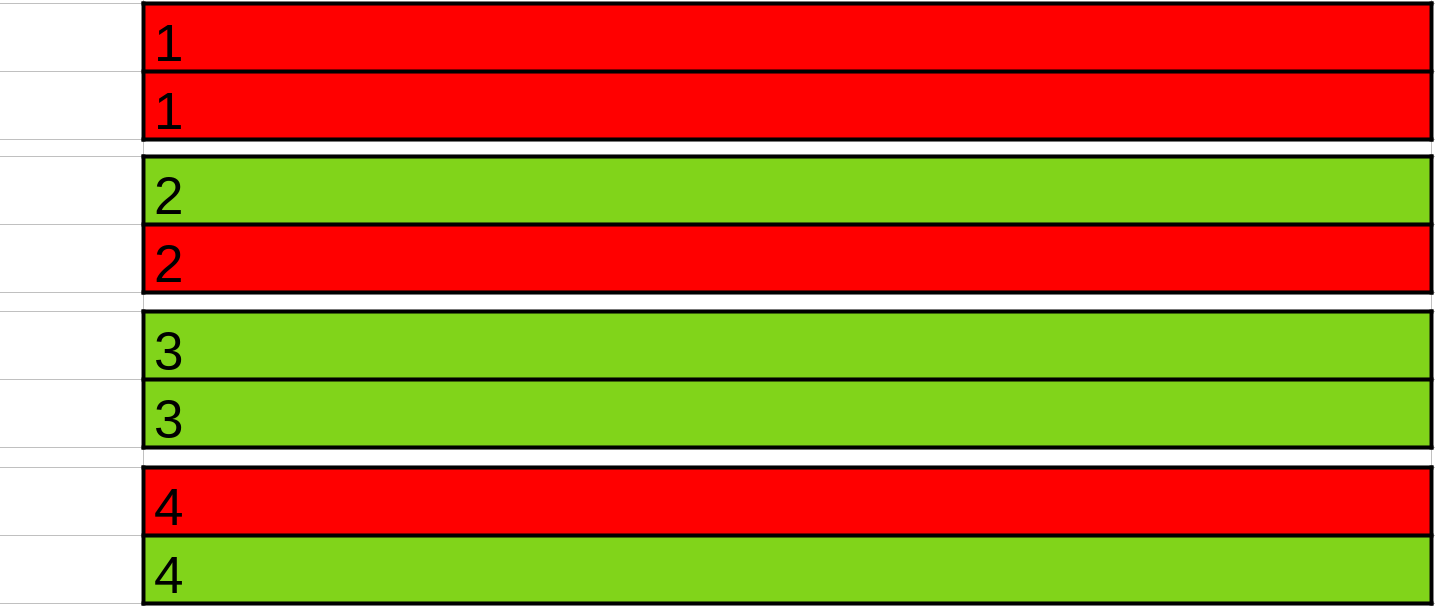
\includegraphics[width=12cm]{nac1.png}}
011111111111110001000011001000101100011111110100
\end{frame}

% Wir haben 4 ansprechbare Mengen, somit brauchen wir 2 bits fuers Caching
\begin{frame}
\frametitle{M\"oglichkeit 3: $n$-way Associative Cache (hier $n=2$)}
\centerline{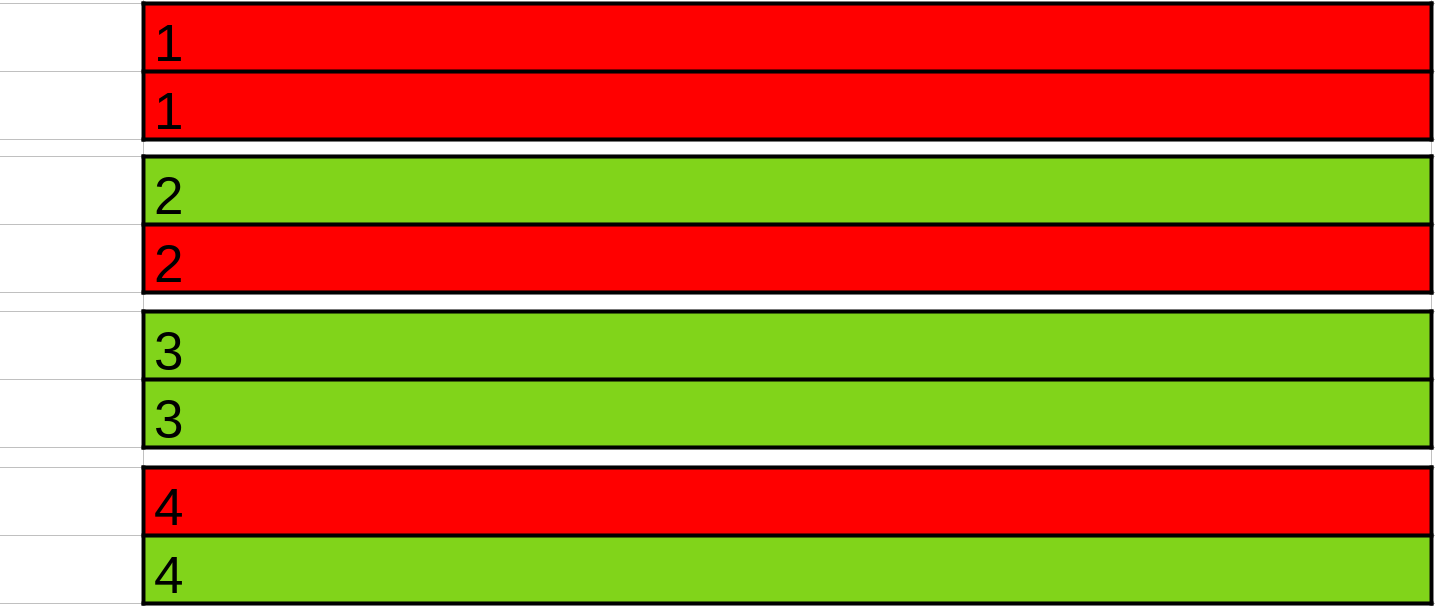
\includegraphics[width=12cm]{nac1.png}}
011111111111110001000011001000101100011111 {\color{orange}110100}
\end{frame}

% Und der Rest ist wieder nur unser Check, um zu gucken ob das wirklich die gewollte Adresse ist
\begin{frame}
\frametitle{M\"oglichkeit 3: $n$-way Associative Cache (hier $n=2$)}
\centerline{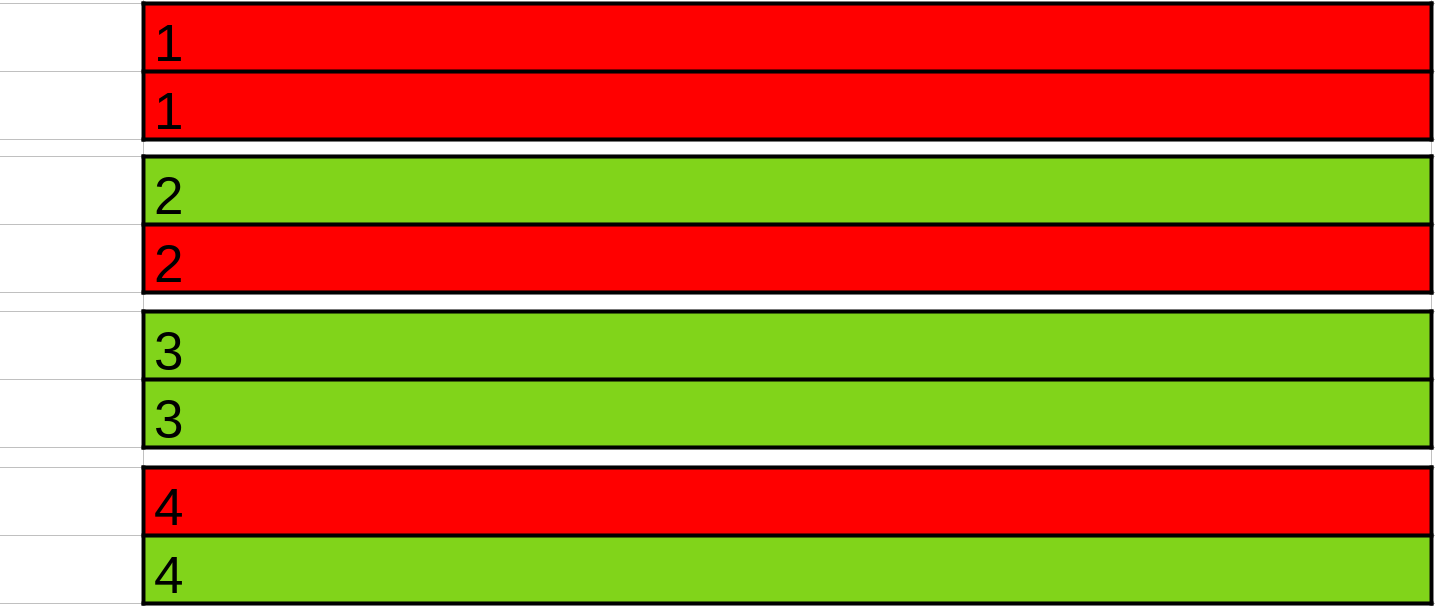
\includegraphics[width=12cm]{nac1.png}}
0111111111111100010000110010001011000111 {\color{blue}11} {\color{orange}110100}
\end{frame}

% Wandeln wir es nun wieder in Binaer um
\begin{frame}
\frametitle{M\"oglichkeit 3: $n$-way Associative Cache (hier $n=2$)}
\centerline{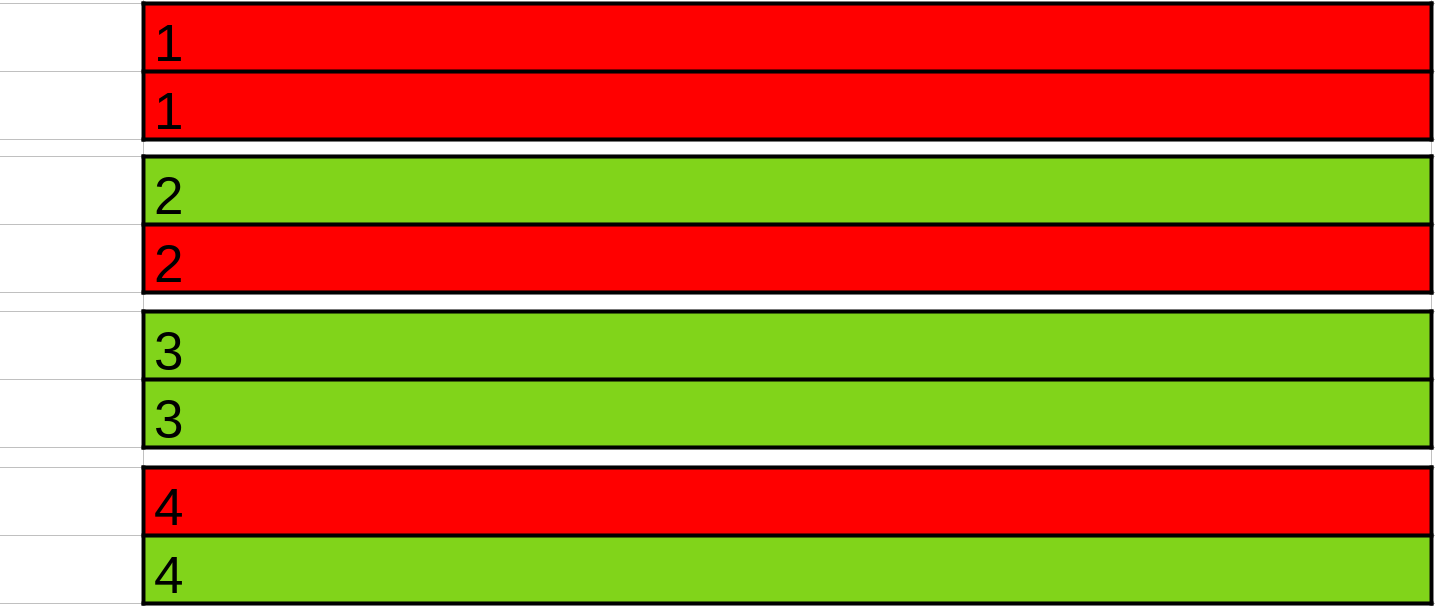
\includegraphics[width=12cm]{nac1.png}}
{\color{brown}0111111111111100010000110010001011000111} {\color{blue}11} {\color{orange}110100}
\end{frame}

% Und nun koennen wir es an Stelle 4 (0 based indexing) speichern.
\begin{frame}
\frametitle{M\"oglichkeit 3: $n$-way Associative Cache (hier $n=2$)}
\centerline{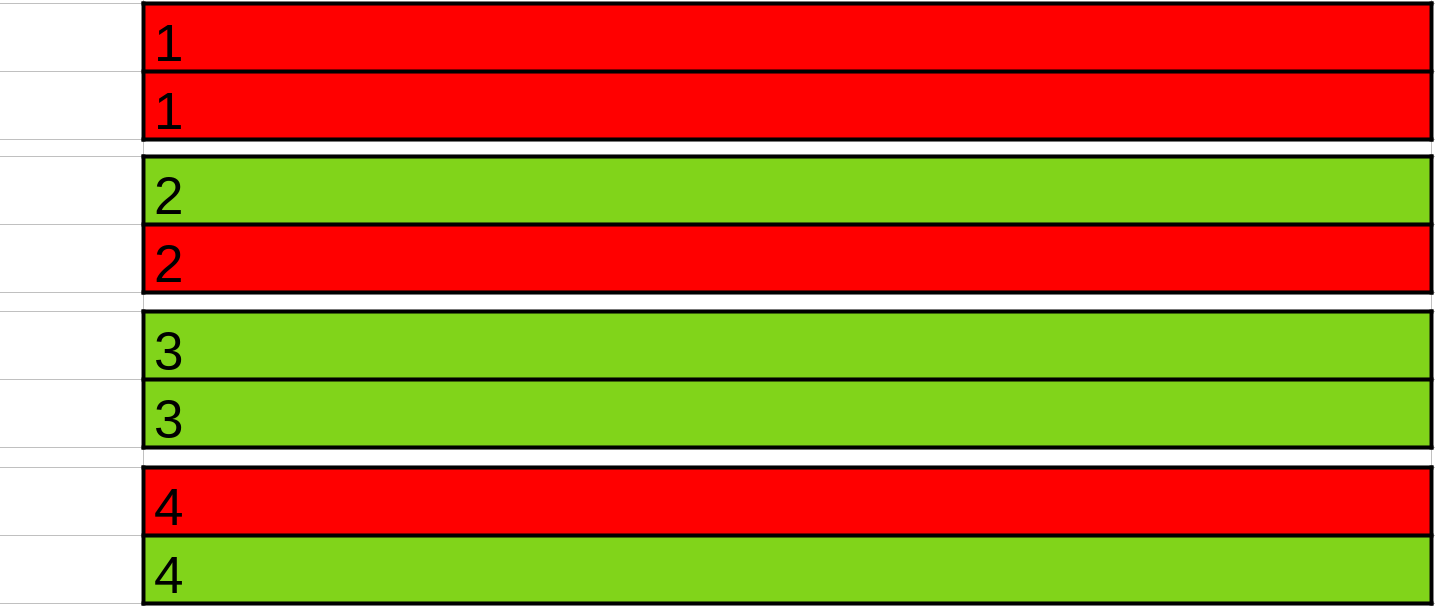
\includegraphics[width=12cm]{nac1.png}}
{\color{brown}549.693.104.839} {\color{blue}3} {\color{orange}52}
\end{frame}

% Okay, cool! Das wird dann auch in der Realitaet genutzt.
% Lasst uns nochmal kurz wiederholen:
\begin{frame}
\frametitle{M\"oglichkeit 3: $n$-way Associative Cache (hier $n=2$)}
\centerline{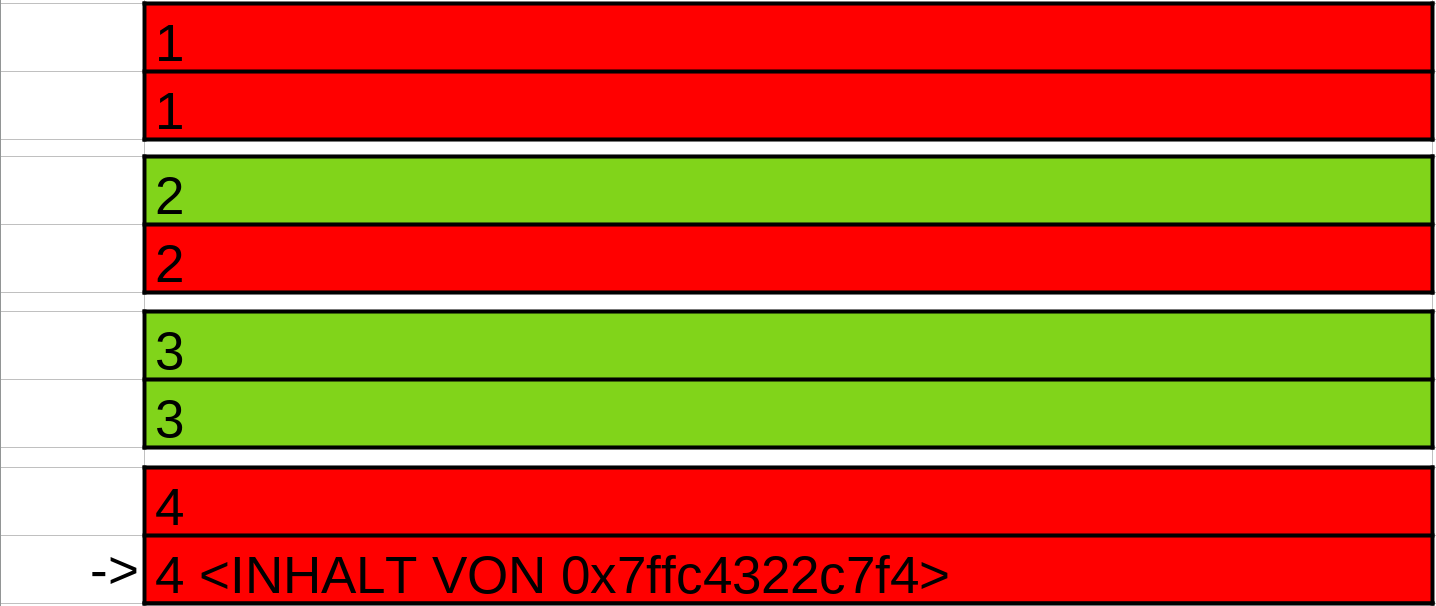
\includegraphics[width=12cm]{nac2.png}}
{\color{brown}549.693.104.839} {\color{blue}3} {\color{orange}52}
\end{frame}

% Am Ende:
%   - Damit sich der Kreis schliesst
\begin{frame}
\frametitle{\"Uberblick Cache Associativity}
Es gibt
\begin{itemize}
    \pause
    \item \textbf{Fully Associative} wo frei zuordbar und alles gecheckt werden muss
    \pause
    \item \textbf{Direct Mapped}, wo mit Hashing eindeutig zugeordnet wird
    \pause
    \item \textbf{$n$-way Associative Cache} Es gibt Mengen der L\"ange $n$
    \pause
    \begin{itemize}
        \item Zwischen den Mengen wird Directly Mapped (gehasht)
        \pause
        \item Innerhalb der Mengen ist es Fully Associative
    \end{itemize}
\end{itemize}
\end{frame}



% Die Theorie ist ja cool und so, aber...
%
% Erwaehnen, dass es der letzte Punkt ist.
%
% Lasst uns noch schnell ueber 3 simple Moeglichkeiten gehen.
\begin{frame}
\centering
{
\Huge Sooooooooooo\\~\\
}
\pause
Wie kann man den Cache optimieren?
\end{frame}

% Structs aufbrechen:
%   - Wenn ihr manches oft braucht, manches selten, dann 
%   - Weniger structs brauchen weniger Speicher
%     - Weniger Speicher braucht weniger Cache Lines
%     - Weniger Cache Lines heisst mehr Platz zum Cachen
%     - Und es heisst auch, dass man weniger Kollisionen hat
%
% 


% So, der Code sieht okay aus oder?
%
% pahole (kurz: PokeAHole) ist ein Tool, das automatisch nach structs analysiert und nach Loechern sucht.
% Was genau Loecher sind und warum sie auftreten zeige ich gleich.
\begin{frame}{Optimierung 1: \texttt{struct}s umstrukturieren!}
Gucken wir uns mal folgenden Code an:
\centerline{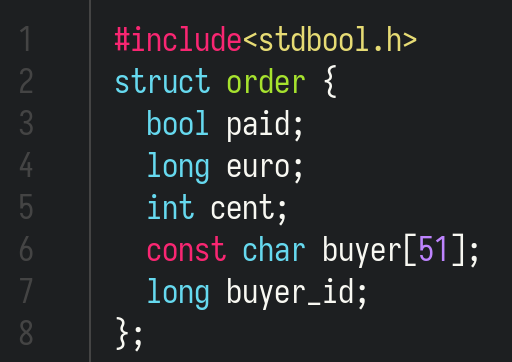
\includegraphics[height=6cm]{example1.png}}
\pause
Lassen wir \texttt{pahole} mal dr\"uberschauen!
\end{frame}


% Zuerst muessen wir unser C-Programm mit der debug flag kompilieren
\begin{frame}{Optimierung 1: \texttt{pahole} zur Rettung!}
\centerline{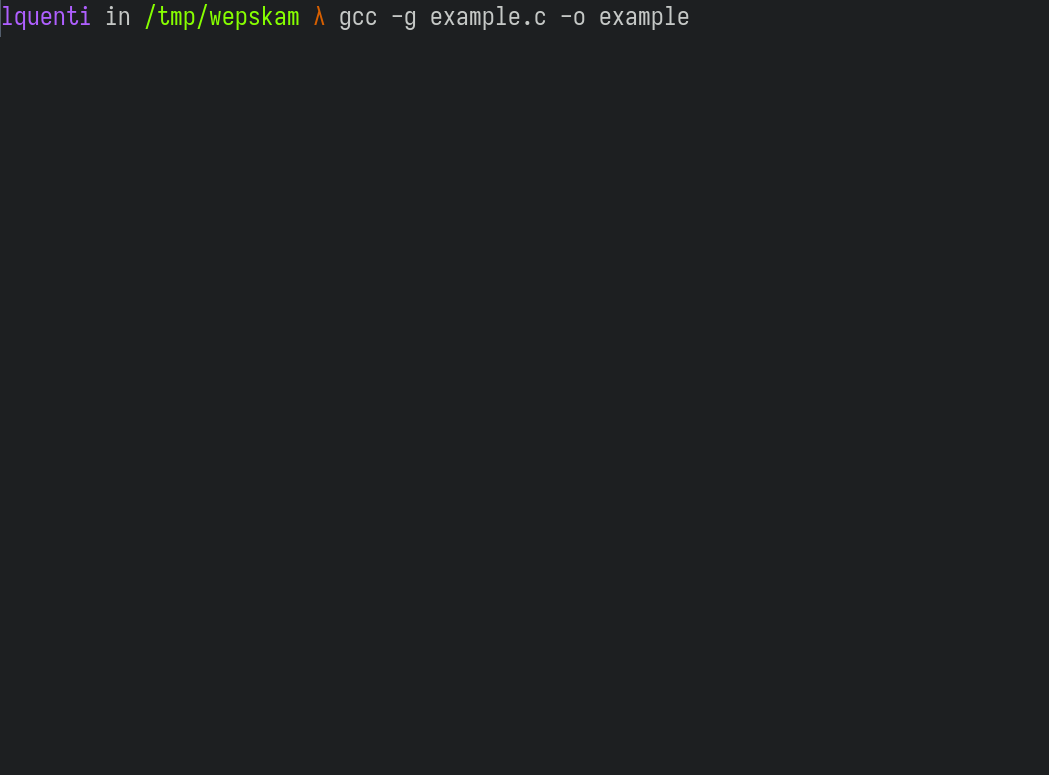
\includegraphics[height=6cm]{example2.png}}
\end{frame}

% Dann sagen wir pahole, dass wir die class (struct) order angucken wollen.
% bat ist einfach ne cat-alternative die uns das schoen formatiert
\begin{frame}{Optimierung 1: \texttt{pahole} zur Rettung!}
\centerline{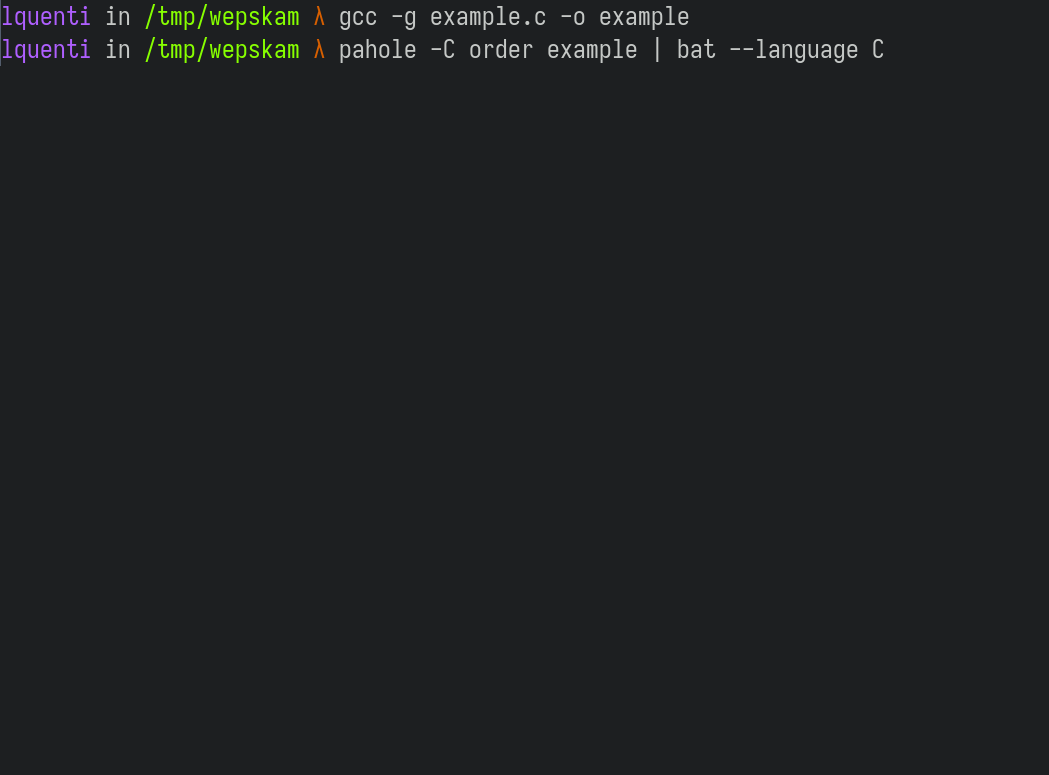
\includegraphics[height=6cm]{example3.png}}
\end{frame}

% Man achte auf line 4:
% Hier ist ein Loch von 7 bytes.
% Warum?
% Der CPU braucht sogenanntes "data structure alignment".
% Das heisst, dass jeder Datentyp immer am Anfang von den Byteschritten sein muss.
% Sprich, bei uns ist ein int 4 bytes. Das heisst, dass es am Anfang jeder 4 bytes anfangen muss.
% Sprich byte 0 waere okay, byte 1-2-3 nicht, byte 4 wieder, dann byte 8 und so weiter.
%
% Nun haben wir hier unseren boolean, der 1 byte gross ist.
% Danach kommt ein Double, der 8 byte gross ist.
% Weil der double aligned sein muss, darf er nur an Stellen 0,8,16,24,32 kommen
% somit muessen byte 2-7 freigelassen werden, was Platzverschwendung ist!
%
% ABER HIER HOERT ES NOCH GAR NICHT AUF!
\begin{frame}{Optimierung 1: \texttt{pahole} zur Rettung!}
\centerline{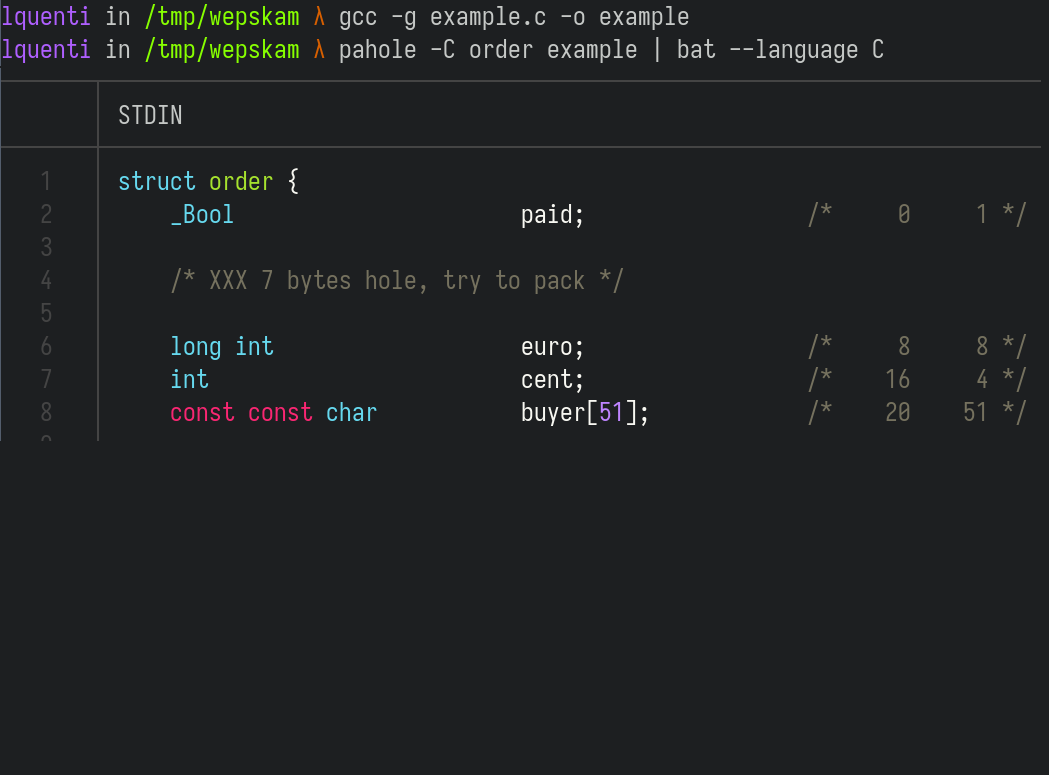
\includegraphics[height=6cm]{example4.png}}
\end{frame}

% In zeile 12 sehen wir, dass die erste cache line voll ist.
% Jedoch nutzen wir in der 2. line fuer unser Struct nur 16 von 64 byte.
%
% Angenommen, uns interessiert meistens nur wie viel eingenommen wurde.
% Dann reicht es ja, nur paid, euro und cent zu haben.
%
% Wenn man dann das struct aufbricht, kriegt man doppelt so viele Bestellungen in den L1 Cache!
\begin{frame}{Optimierung 1: \texttt{pahole} zur Rettung!}
\centerline{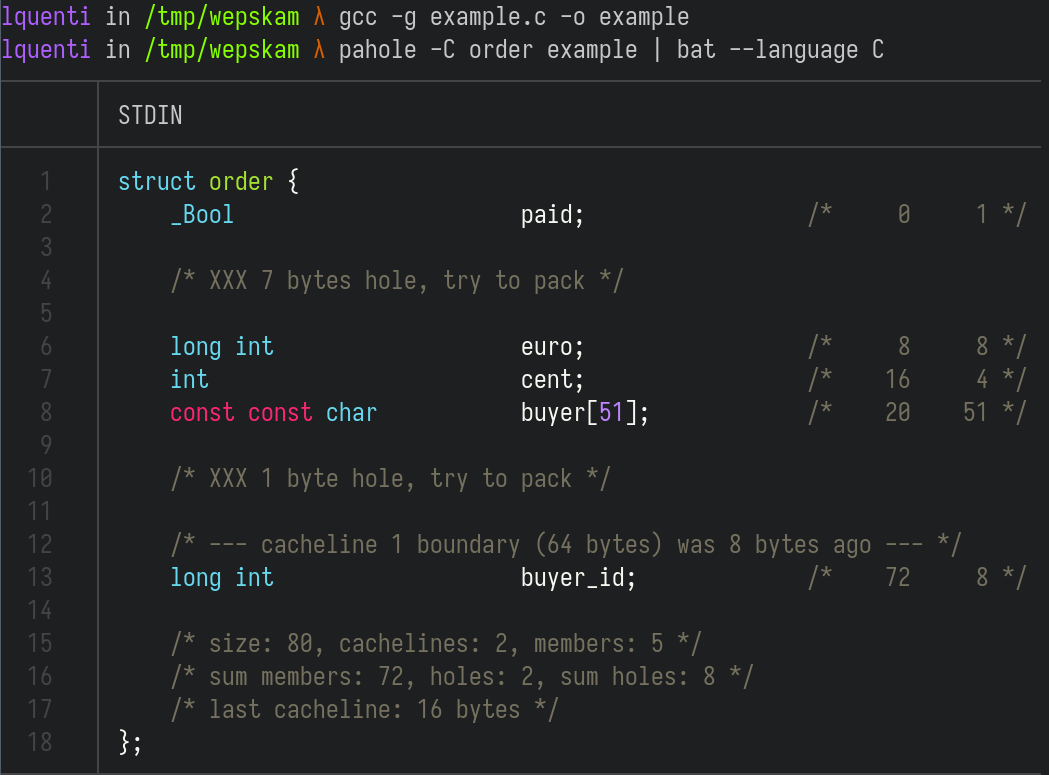
\includegraphics[height=6cm]{example5.png}}
\end{frame}

% Warum will man Daten nicht in den Cache speichern?
%  - Wenn man weiss, dass man sie eh laenger nicht anfaesst.
%  - Oder wenn man so viele Daten schreibt dass es danach eh wieder weg ist.
%  - Dann schreibt man einfach direkt in den Memory.
% <PAUSE>
% Ich geh nicht weiter darauf ein weil das eww Code ist, aber wenn ihr es braucht wisst ihr dass es
% existiert.
\begin{frame}{Optimerung 2: Non-temporale write operationen.}
Man kann Daten auch direkt in das Memory schreiben.\\
\pause
Der Code wird dann aber eww.\\~\\
\centerline{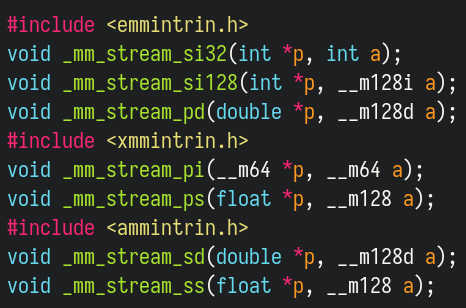
\includegraphics[height=5cm]{nontemporal.png}}
\end{frame}

% Die Leute die Info 2 gehoert haben wissen das bereits.
% Die operands koennen erst gefetched werden wenn man weiss wie viele Operanden die aktuelle
% instruktion braucht!
\begin{frame}{Optimierung 3: Pipelining verbessern}
Eine Instruktion besteht im Prozessor aus 5 Schritten:\\
\begin{enumerate}
    \item Instruction fetch
    \pause
    \item instruction decode
    \pause
    \item operands fetch
    \pause
    \item execute operation
    \pause
    \item operands store
\end{enumerate}
\end{frame}

\begin{frame}{Optimierung 3: Pipelining verbessern}
\centerline{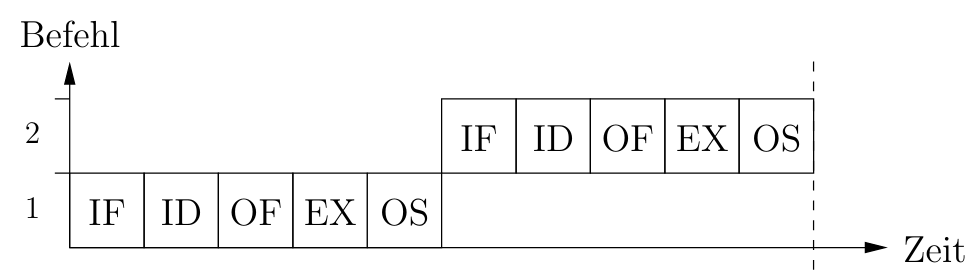
\includegraphics[width=12cm]{if1.png}}
\end{frame}

% Das ist moeglich weil im Prozessor verschiedene Schaltnetze fuer die verschiedenen Sachen
% zustaendig sind
%
% -> Das nennt sich Pipelining
%
% Nun kann dieser nur gut pipelinen wenn er auch wirklich weiss was die naechsten Instruktionen sind.
% Was ist nun, wenn wir an ein if-else kommen? Woher soll der Prozessor wissen ob er den if oder den
% else vorbereiten soll?
%
\begin{frame}{Optimierung 3: Pipelining verbessern}
\centerline{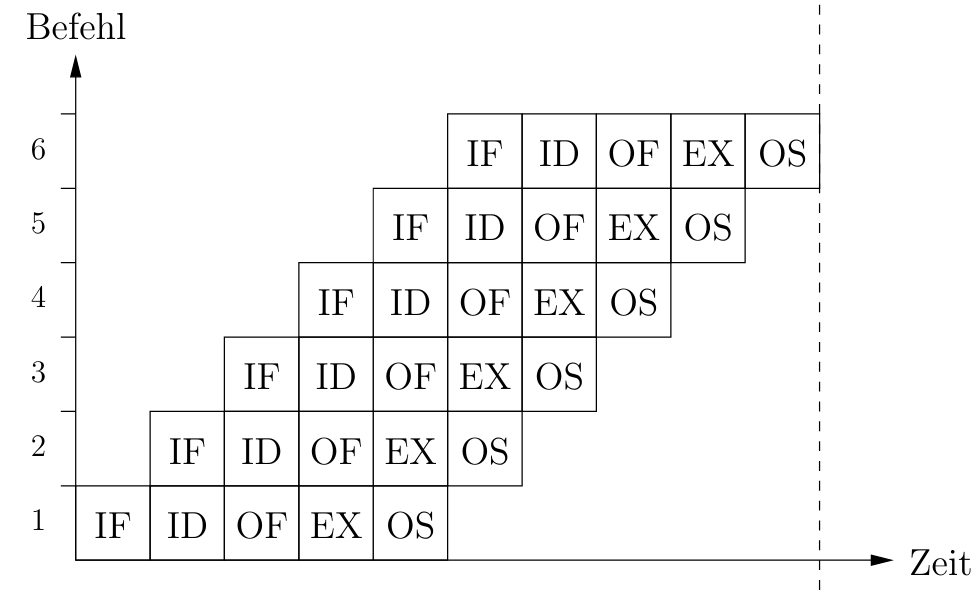
\includegraphics[width=12cm]{if2.png}}
\end{frame}

% Fragt mich bitte nicht in welchen ekeligen Randbedingungen man die Doppelverneinung braucht.
% In JS wird das als implizites bool casting genommen
\begin{frame}{Optimierung 3: Pipelining verbessern}
\centerline{\includegraphics[width=12cm]{likely1.png}}
~\\~\\~\pause~
\centerline{\includegraphics[width=5.5cm]{likely2.png}}
\end{frame}

\begin{frame}{Optimierung 4: Gro\ss{}e Structs aufbrechen}
  \begin{columns}
    \begin{column}{0.5\textwidth}
  \centerline{\includegraphics[width=0.9\textwidth]{breakup1.png}}
    \end{column}
    \pause
    \begin{column}{0.5\textwidth}
  \centerline{\includegraphics[width=0.9\textwidth]{breakup2.png}}
    \end{column}
  \end{columns}
  \pause
  AUCH: Daten nah beieinander halten, wenig Sprünge
\end{frame}

\begin{frame}[t]{Optimierung 5: Ifs vermeiden}
  \centerline{\includegraphics[width=0.7\textwidth]{branchless1.png}}
  \pause
  \centerline{\includegraphics[width=0.7\textwidth]{branchless2.png}}
\end{frame}

\begin{frame}{Falls ihr mehr lernen wollt...}
\begin{columns}
    \begin{column}{0.48\textwidth}
        \centerline{\includegraphics[height=7cm]{paper.png}}
    \end{column}
    \pause
    \begin{column}{0.48\textwidth}
        Was wir ausgelassen haben:
        \begin{itemize}
            \item Elektrotechnik
            \item Non-Uniform Memory Access
            \item Cachesynchronisation zwischen Prozessorkernen
            \item Virtual Memory, Memory Management Unit, Translate Lookaside Buffer
            \item Write cache flushing
        \end{itemize}
    \end{column}
\end{columns}
\end{frame}

\begin{frame}
\centering
{\Huge
Vielen Dank f\"ur die Aufmerksamkeit!
}\\
Fragen?
\end{frame}

\end{document}
